% Options for packages loaded elsewhere
\PassOptionsToPackage{unicode}{hyperref}
\PassOptionsToPackage{hyphens}{url}
\PassOptionsToPackage{dvipsnames,svgnames,x11names}{xcolor}
%
\documentclass[
  a4paper,
  DIV=11,
  numbers=noendperiod]{scrartcl}

\usepackage{amsmath,amssymb}
\usepackage{iftex}
\ifPDFTeX
  \usepackage[T1]{fontenc}
  \usepackage[utf8]{inputenc}
  \usepackage{textcomp} % provide euro and other symbols
\else % if luatex or xetex
  \usepackage{unicode-math}
  \defaultfontfeatures{Scale=MatchLowercase}
  \defaultfontfeatures[\rmfamily]{Ligatures=TeX,Scale=1}
\fi
\usepackage{lmodern}
\ifPDFTeX\else  
    % xetex/luatex font selection
\fi
% Use upquote if available, for straight quotes in verbatim environments
\IfFileExists{upquote.sty}{\usepackage{upquote}}{}
\IfFileExists{microtype.sty}{% use microtype if available
  \usepackage[]{microtype}
  \UseMicrotypeSet[protrusion]{basicmath} % disable protrusion for tt fonts
}{}
\makeatletter
\@ifundefined{KOMAClassName}{% if non-KOMA class
  \IfFileExists{parskip.sty}{%
    \usepackage{parskip}
  }{% else
    \setlength{\parindent}{0pt}
    \setlength{\parskip}{6pt plus 2pt minus 1pt}}
}{% if KOMA class
  \KOMAoptions{parskip=half}}
\makeatother
\usepackage{xcolor}
\usepackage[inner=2.5cm,outer=2.5cm,top=3cm,bottom=4cm,headsep=22pt,headheight=11pt,footskip=33pt,ignorehead,ignorefoot,heightrounded]{geometry}
\setlength{\emergencystretch}{3em} % prevent overfull lines
\setcounter{secnumdepth}{5}
% Make \paragraph and \subparagraph free-standing
\makeatletter
\ifx\paragraph\undefined\else
  \let\oldparagraph\paragraph
  \renewcommand{\paragraph}{
    \@ifstar
      \xxxParagraphStar
      \xxxParagraphNoStar
  }
  \newcommand{\xxxParagraphStar}[1]{\oldparagraph*{#1}\mbox{}}
  \newcommand{\xxxParagraphNoStar}[1]{\oldparagraph{#1}\mbox{}}
\fi
\ifx\subparagraph\undefined\else
  \let\oldsubparagraph\subparagraph
  \renewcommand{\subparagraph}{
    \@ifstar
      \xxxSubParagraphStar
      \xxxSubParagraphNoStar
  }
  \newcommand{\xxxSubParagraphStar}[1]{\oldsubparagraph*{#1}\mbox{}}
  \newcommand{\xxxSubParagraphNoStar}[1]{\oldsubparagraph{#1}\mbox{}}
\fi
\makeatother

\usepackage{color}
\usepackage{fancyvrb}
\newcommand{\VerbBar}{|}
\newcommand{\VERB}{\Verb[commandchars=\\\{\}]}
\DefineVerbatimEnvironment{Highlighting}{Verbatim}{commandchars=\\\{\}}
% Add ',fontsize=\small' for more characters per line
\usepackage{framed}
\definecolor{shadecolor}{RGB}{241,243,245}
\newenvironment{Shaded}{\begin{snugshade}}{\end{snugshade}}
\newcommand{\AlertTok}[1]{\textcolor[rgb]{0.68,0.00,0.00}{#1}}
\newcommand{\AnnotationTok}[1]{\textcolor[rgb]{0.37,0.37,0.37}{#1}}
\newcommand{\AttributeTok}[1]{\textcolor[rgb]{0.40,0.45,0.13}{#1}}
\newcommand{\BaseNTok}[1]{\textcolor[rgb]{0.68,0.00,0.00}{#1}}
\newcommand{\BuiltInTok}[1]{\textcolor[rgb]{0.00,0.23,0.31}{#1}}
\newcommand{\CharTok}[1]{\textcolor[rgb]{0.13,0.47,0.30}{#1}}
\newcommand{\CommentTok}[1]{\textcolor[rgb]{0.37,0.37,0.37}{#1}}
\newcommand{\CommentVarTok}[1]{\textcolor[rgb]{0.37,0.37,0.37}{\textit{#1}}}
\newcommand{\ConstantTok}[1]{\textcolor[rgb]{0.56,0.35,0.01}{#1}}
\newcommand{\ControlFlowTok}[1]{\textcolor[rgb]{0.00,0.23,0.31}{\textbf{#1}}}
\newcommand{\DataTypeTok}[1]{\textcolor[rgb]{0.68,0.00,0.00}{#1}}
\newcommand{\DecValTok}[1]{\textcolor[rgb]{0.68,0.00,0.00}{#1}}
\newcommand{\DocumentationTok}[1]{\textcolor[rgb]{0.37,0.37,0.37}{\textit{#1}}}
\newcommand{\ErrorTok}[1]{\textcolor[rgb]{0.68,0.00,0.00}{#1}}
\newcommand{\ExtensionTok}[1]{\textcolor[rgb]{0.00,0.23,0.31}{#1}}
\newcommand{\FloatTok}[1]{\textcolor[rgb]{0.68,0.00,0.00}{#1}}
\newcommand{\FunctionTok}[1]{\textcolor[rgb]{0.28,0.35,0.67}{#1}}
\newcommand{\ImportTok}[1]{\textcolor[rgb]{0.00,0.46,0.62}{#1}}
\newcommand{\InformationTok}[1]{\textcolor[rgb]{0.37,0.37,0.37}{#1}}
\newcommand{\KeywordTok}[1]{\textcolor[rgb]{0.00,0.23,0.31}{\textbf{#1}}}
\newcommand{\NormalTok}[1]{\textcolor[rgb]{0.00,0.23,0.31}{#1}}
\newcommand{\OperatorTok}[1]{\textcolor[rgb]{0.37,0.37,0.37}{#1}}
\newcommand{\OtherTok}[1]{\textcolor[rgb]{0.00,0.23,0.31}{#1}}
\newcommand{\PreprocessorTok}[1]{\textcolor[rgb]{0.68,0.00,0.00}{#1}}
\newcommand{\RegionMarkerTok}[1]{\textcolor[rgb]{0.00,0.23,0.31}{#1}}
\newcommand{\SpecialCharTok}[1]{\textcolor[rgb]{0.37,0.37,0.37}{#1}}
\newcommand{\SpecialStringTok}[1]{\textcolor[rgb]{0.13,0.47,0.30}{#1}}
\newcommand{\StringTok}[1]{\textcolor[rgb]{0.13,0.47,0.30}{#1}}
\newcommand{\VariableTok}[1]{\textcolor[rgb]{0.07,0.07,0.07}{#1}}
\newcommand{\VerbatimStringTok}[1]{\textcolor[rgb]{0.13,0.47,0.30}{#1}}
\newcommand{\WarningTok}[1]{\textcolor[rgb]{0.37,0.37,0.37}{\textit{#1}}}

\providecommand{\tightlist}{%
  \setlength{\itemsep}{0pt}\setlength{\parskip}{0pt}}\usepackage{longtable,booktabs,array}
\usepackage{calc} % for calculating minipage widths
% Correct order of tables after \paragraph or \subparagraph
\usepackage{etoolbox}
\makeatletter
\patchcmd\longtable{\par}{\if@noskipsec\mbox{}\fi\par}{}{}
\makeatother
% Allow footnotes in longtable head/foot
\IfFileExists{footnotehyper.sty}{\usepackage{footnotehyper}}{\usepackage{footnote}}
\makesavenoteenv{longtable}
\usepackage{graphicx}
\makeatletter
\def\maxwidth{\ifdim\Gin@nat@width>\linewidth\linewidth\else\Gin@nat@width\fi}
\def\maxheight{\ifdim\Gin@nat@height>\textheight\textheight\else\Gin@nat@height\fi}
\makeatother
% Scale images if necessary, so that they will not overflow the page
% margins by default, and it is still possible to overwrite the defaults
% using explicit options in \includegraphics[width, height, ...]{}
\setkeys{Gin}{width=\maxwidth,height=\maxheight,keepaspectratio}
% Set default figure placement to htbp
\makeatletter
\def\fps@figure{htbp}
\makeatother
% definitions for citeproc citations
\NewDocumentCommand\citeproctext{}{}
\NewDocumentCommand\citeproc{mm}{%
  \begingroup\def\citeproctext{#2}\cite{#1}\endgroup}
\makeatletter
 % allow citations to break across lines
 \let\@cite@ofmt\@firstofone
 % avoid brackets around text for \cite:
 \def\@biblabel#1{}
 \def\@cite#1#2{{#1\if@tempswa , #2\fi}}
\makeatother
\newlength{\cslhangindent}
\setlength{\cslhangindent}{1.5em}
\newlength{\csllabelwidth}
\setlength{\csllabelwidth}{3em}
\newenvironment{CSLReferences}[2] % #1 hanging-indent, #2 entry-spacing
 {\begin{list}{}{%
  \setlength{\itemindent}{0pt}
  \setlength{\leftmargin}{0pt}
  \setlength{\parsep}{0pt}
  % turn on hanging indent if param 1 is 1
  \ifodd #1
   \setlength{\leftmargin}{\cslhangindent}
   \setlength{\itemindent}{-1\cslhangindent}
  \fi
  % set entry spacing
  \setlength{\itemsep}{#2\baselineskip}}}
 {\end{list}}
\usepackage{calc}
\newcommand{\CSLBlock}[1]{\hfill\break\parbox[t]{\linewidth}{\strut\ignorespaces#1\strut}}
\newcommand{\CSLLeftMargin}[1]{\parbox[t]{\csllabelwidth}{\strut#1\strut}}
\newcommand{\CSLRightInline}[1]{\parbox[t]{\linewidth - \csllabelwidth}{\strut#1\strut}}
\newcommand{\CSLIndent}[1]{\hspace{\cslhangindent}#1}

\KOMAoption{captions}{tableheading}
\makeatletter
\@ifpackageloaded{tcolorbox}{}{\usepackage[skins,breakable]{tcolorbox}}
\@ifpackageloaded{fontawesome5}{}{\usepackage{fontawesome5}}
\definecolor{quarto-callout-color}{HTML}{909090}
\definecolor{quarto-callout-note-color}{HTML}{0758E5}
\definecolor{quarto-callout-important-color}{HTML}{CC1914}
\definecolor{quarto-callout-warning-color}{HTML}{EB9113}
\definecolor{quarto-callout-tip-color}{HTML}{00A047}
\definecolor{quarto-callout-caution-color}{HTML}{FC5300}
\definecolor{quarto-callout-color-frame}{HTML}{acacac}
\definecolor{quarto-callout-note-color-frame}{HTML}{4582ec}
\definecolor{quarto-callout-important-color-frame}{HTML}{d9534f}
\definecolor{quarto-callout-warning-color-frame}{HTML}{f0ad4e}
\definecolor{quarto-callout-tip-color-frame}{HTML}{02b875}
\definecolor{quarto-callout-caution-color-frame}{HTML}{fd7e14}
\makeatother
\makeatletter
\@ifpackageloaded{caption}{}{\usepackage{caption}}
\AtBeginDocument{%
\ifdefined\contentsname
  \renewcommand*\contentsname{Table of contents}
\else
  \newcommand\contentsname{Table of contents}
\fi
\ifdefined\listfigurename
  \renewcommand*\listfigurename{List of Figures}
\else
  \newcommand\listfigurename{List of Figures}
\fi
\ifdefined\listtablename
  \renewcommand*\listtablename{List of Tables}
\else
  \newcommand\listtablename{List of Tables}
\fi
\ifdefined\figurename
  \renewcommand*\figurename{Figure}
\else
  \newcommand\figurename{Figure}
\fi
\ifdefined\tablename
  \renewcommand*\tablename{Table}
\else
  \newcommand\tablename{Table}
\fi
}
\@ifpackageloaded{float}{}{\usepackage{float}}
\floatstyle{ruled}
\@ifundefined{c@chapter}{\newfloat{codelisting}{h}{lop}}{\newfloat{codelisting}{h}{lop}[chapter]}
\floatname{codelisting}{Listing}
\newcommand*\listoflistings{\listof{codelisting}{List of Listings}}
\makeatother
\makeatletter
\makeatother
\makeatletter
\@ifpackageloaded{caption}{}{\usepackage{caption}}
\@ifpackageloaded{subcaption}{}{\usepackage{subcaption}}
\makeatother

\ifLuaTeX
  \usepackage{selnolig}  % disable illegal ligatures
\fi
\usepackage{bookmark}

\IfFileExists{xurl.sty}{\usepackage{xurl}}{} % add URL line breaks if available
\urlstyle{same} % disable monospaced font for URLs
\hypersetup{
  pdftitle={IEC Wind Turbine Type 3 (Doubly-Fed Induction Generator)},
  pdfauthor={Martin Franke (Fraunhofer IEE), Luka Plavec (Fraunhofer IEE)},
  colorlinks=true,
  linkcolor={blue},
  filecolor={Maroon},
  citecolor={Blue},
  urlcolor={Blue},
  pdfcreator={LaTeX via pandoc}}


\title{IEC Wind Turbine Type 3 (Doubly-Fed Induction Generator)}
\author{Martin Franke (Fraunhofer IEE), Luka Plavec (Fraunhofer IEE)}
\date{}

\begin{document}
\maketitle

\renewcommand*\contentsname{Table of contents}
{
\hypersetup{linkcolor=}
\setcounter{tocdepth}{3}
\tableofcontents
}
\listoffigures
\listoftables

\section{List Of Acronyms}\label{acronyms_HEADER_LOA}

\begin{description}
\tightlist
\item[\phantomsection\label{acronyms_DFIG}{DFIG}]
Doubly-Fed Induction Generator
\item[\phantomsection\label{acronyms_FRT}{FRT}]
Fault Ride Through
\item[\phantomsection\label{acronyms_GSC}{GSC}]
Grid Side Converter
\item[\phantomsection\label{acronyms_PCC}{PCC}]
Point of Common Coupling
\item[\phantomsection\label{acronyms_PD}{PD}]
Power Device
\item[\phantomsection\label{acronyms_RSC}{RSC}]
Rotor Side Converter
\item[\phantomsection\label{acronyms_WP}{WP}]
Wind Plant
\item[\phantomsection\label{acronyms_WT}{WT}]
Wind Turbine
\end{description}

\section{Context}\label{context}

This document refers to the IEC 61400-27-1 models which have been
developed with the following specifications in mind {[}1{]}:

\begin{itemize}
\item
  Use in wind power plant models or standalone wind turbines
\item
  Specification for generic simulation models covering most WT types
\item
  Models address four categories of existing WT technologies (NERC
  nomenclature):

  \begin{itemize}
  \tightlist
  \item
    \textbf{Type 1:} Conventional asynchronous generators (squirrel
    cage)
  \item
    \textbf{Type 2:} Variable rotor resistance asynchronous generators
  \item
    \textbf{Type 3:} Doubly-fed induction generators (stator connected
    directly; rotor through converter)
  \item
    \textbf{Type 4:} Synchronous generator, grid-connected via a
    full-size power converter
  \end{itemize}
\end{itemize}

Other model considerations according to {[}1{]}:

\begin{itemize}
\tightlist
\item
  Include over/under frequency and voltage protection for realistic WT
  disconnection modeling
\item
  Account for turbine-generator inertia and first drive train torsional
  mode impacts on power swings
\item
  Phase-locked loop dynamics are not included in the models (they are
  modeled through a first order lag element)
\end{itemize}

The IEC 61400-27-1 {[}1{]} defines one of the most widely used series of
RMS models for Wind Turbine (WT) generators, another one being the WECC
model series, developed by EPRI.

The models are separated in several sub systems. The information and
drawings are taken from {[}1{]} {[}2{]} {[}3{]} {[}4{]} {[}5{]} {[}6{]}.

\section{Model use, assumptions, validity domain and
limitations}\label{model-use-assumptions-validity-domain-and-limitations}

The controller of the generic Type 3 WT model does not represent the
actual controller of the WT, which sets the references of the
Rotor Side Converter (RSC) and the Grid Side Converter (GSC), but
provides the current command signals to obtain an accurate response of
active and reactive power, observed from the grid side.

The models are positive-sequence RMS models, hence they assume
symmetrical operating conditions and neglect high-frequency dynamics.
This type of models is often used in large-scale stability studies, for
which it reflects the relevant phenomena. It is not a detailed physical
model of the unit. Also for some stability phenomena (e.g.~resonance
stability) this model is not sufficient and EMT models or other
approaches may be necessary.

Specifically, {[}1{]} defines the following validity domain:

\begin{itemize}
\tightlist
\item
  positive sequence dynamics
\item
  transmission grid simulations
\item
  reference value changes
\item
  steady state voltage deviations (0.85 pu \ldots{} 1.15 pu)
\item
  phase jumps
\item
  symmetrical faults, including short-circuits of varying impedance,
  where voltage can dip to close to zero (typical e.g.~0.18 pu)
\item
  frequency disturbances, variations \(\pm\) 6 \%
\item
  electromechanical modes of synchronous generator rotor oscillations
  (0.2 Hz \ldots{} 4 Hz)
\item
  Typical simulation time frame: 10 s \ldots{} 30 s
\item
  Wind speed assumed to be constant during simulation time (wind speed
  could be included as an external condition through the available
  power)
\item
  Simulation step width up to 1/4 fundamental frequency cycle (5 ms at
  50 Hz), which implies that the model Bandwidth cannot be above 15 Hz.
\item
  According to {[}2{]}, the Type 3 WT model can operate with variable
  speed with slip values from -0.3 to +0.4.
\end{itemize}

Vice versa, {[}1{]} states that the models are not intended for the
following:

\begin{itemize}
\tightlist
\item
  The models are not designed for long-term stability assessments.
\item
  The models do not facilitate the exploration of sub-synchronous
  interaction phenomena.
\item
  The models do not account for fluctuations due to wind speed
  variability over time and space, excluding factors such as turbulence,
  tower shadow, wind shear, and wakes.
\item
  The models do not encompass phenomena like harmonics, flicker, or
  other EMC emissions outlined in the IEC 61000 series.
\item
  Linearization for eigenvalue analysis is complex and may not be
  suitable for these simplified models.
\item
  The IEC standard does not cover the details of short-circuit
  calculations.
\item
  The models are not suitable for analyzing extremely weak systems,
  including scenarios where wind turbines operate in isolation from
  other synchronous generation or in cases with very low short-circuit
  ratios.
\item
  The models do not incorporate negative and zero sequence components.
\end{itemize}

\section{Wind turbine type 3}\label{wind-turbine-type-3}

\begin{figure}

\centering{

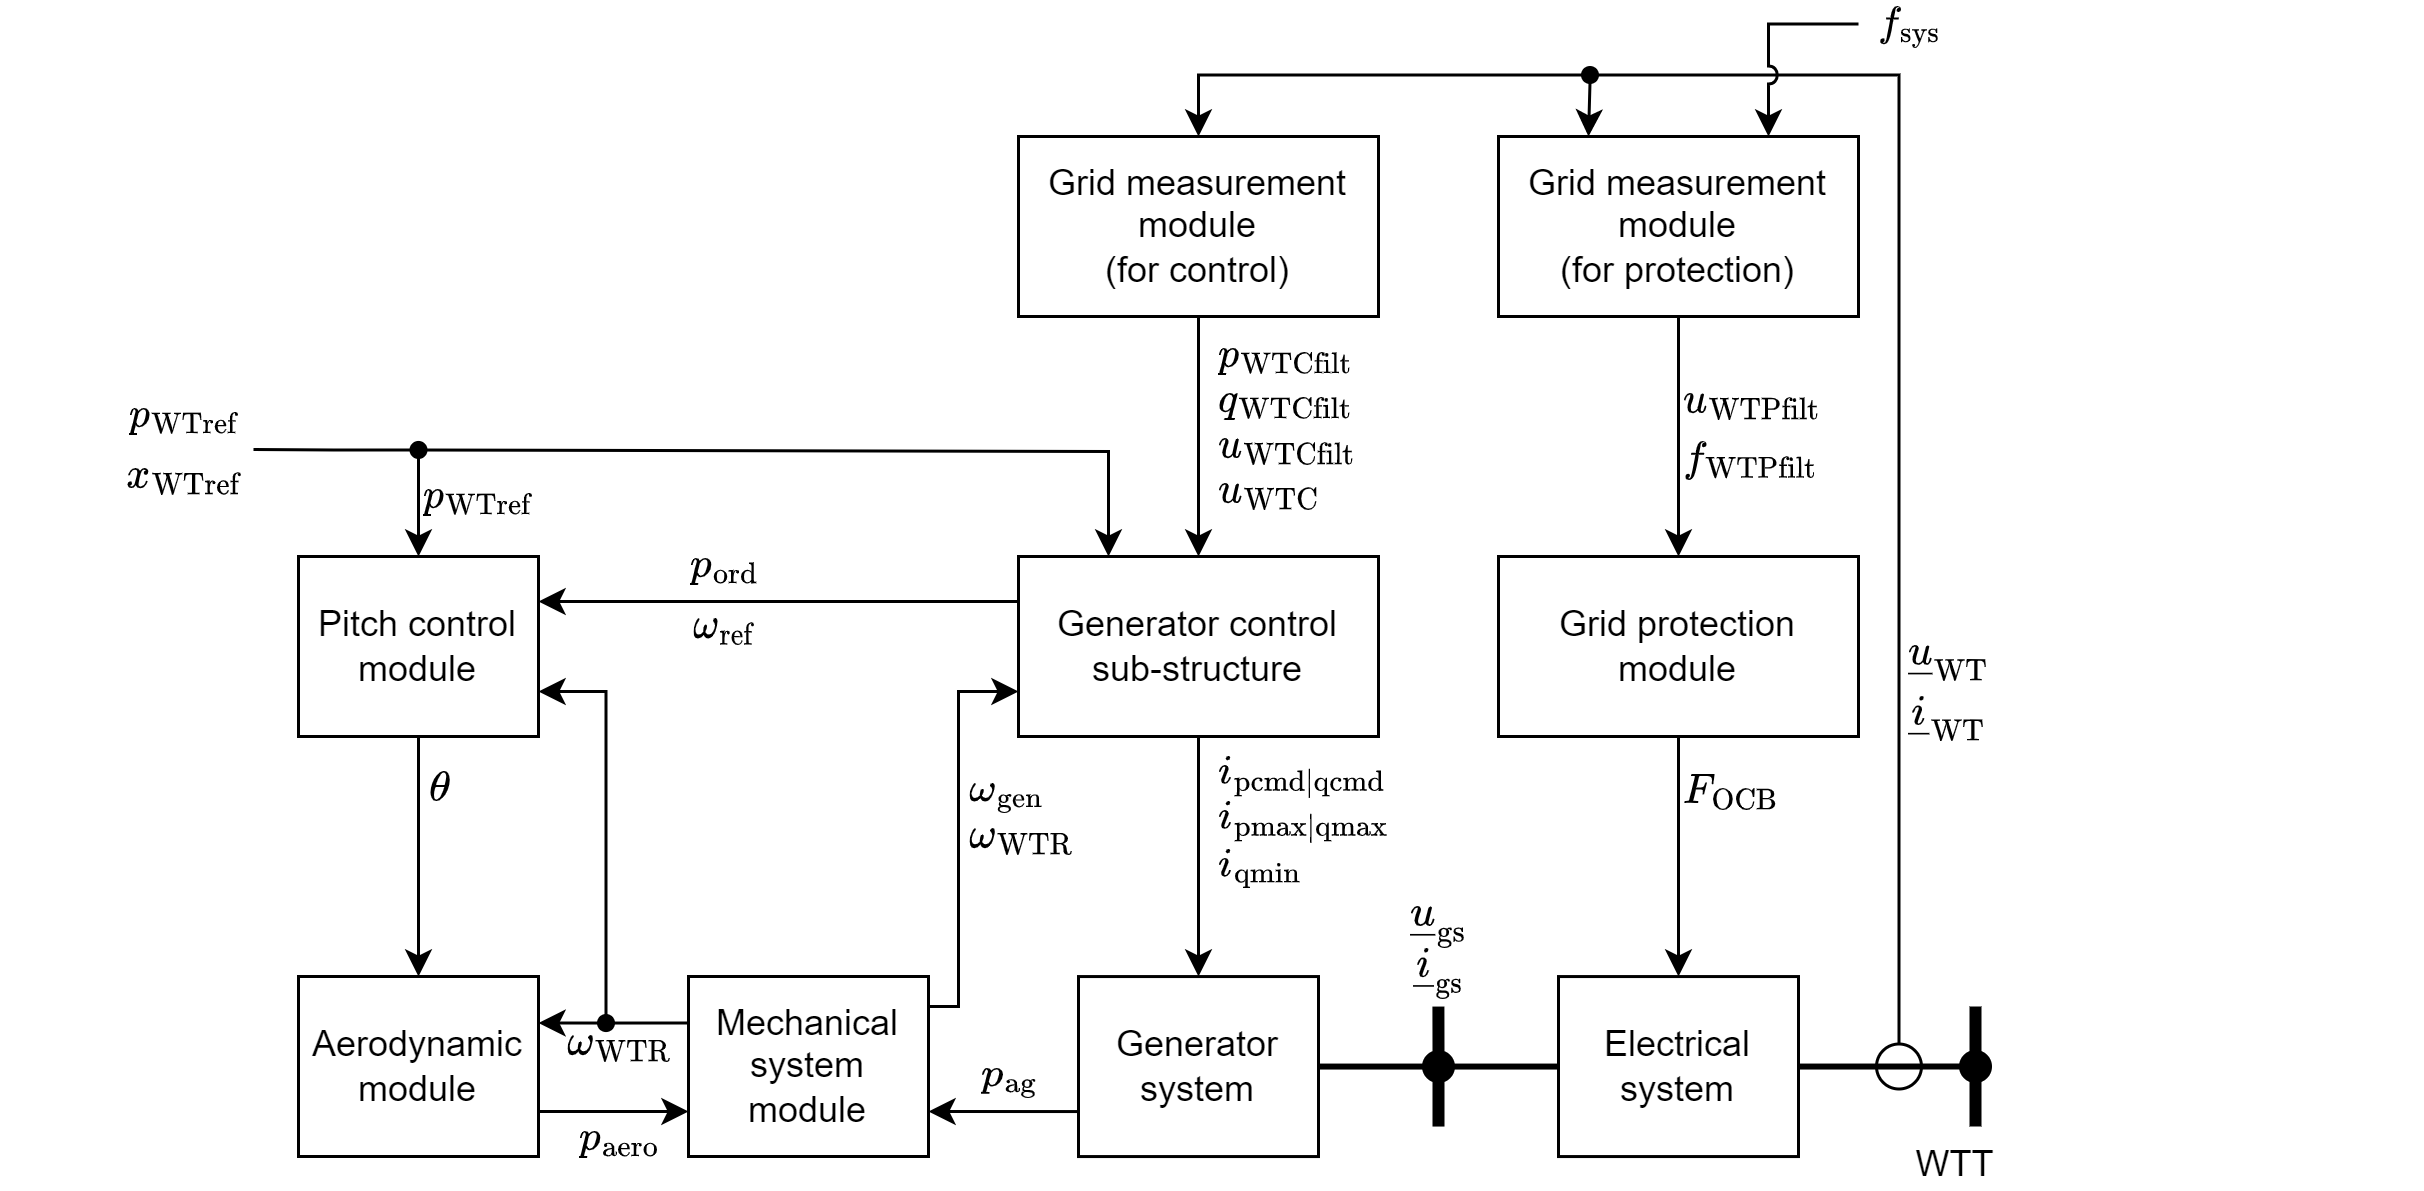
\includegraphics{drawings/WT_system.drawio.png}

}

\caption{\label{fig-wtSystem}Wind turbine type 3 model, based on
{[}1{]}}

\end{figure}%

\begin{figure}

\centering{

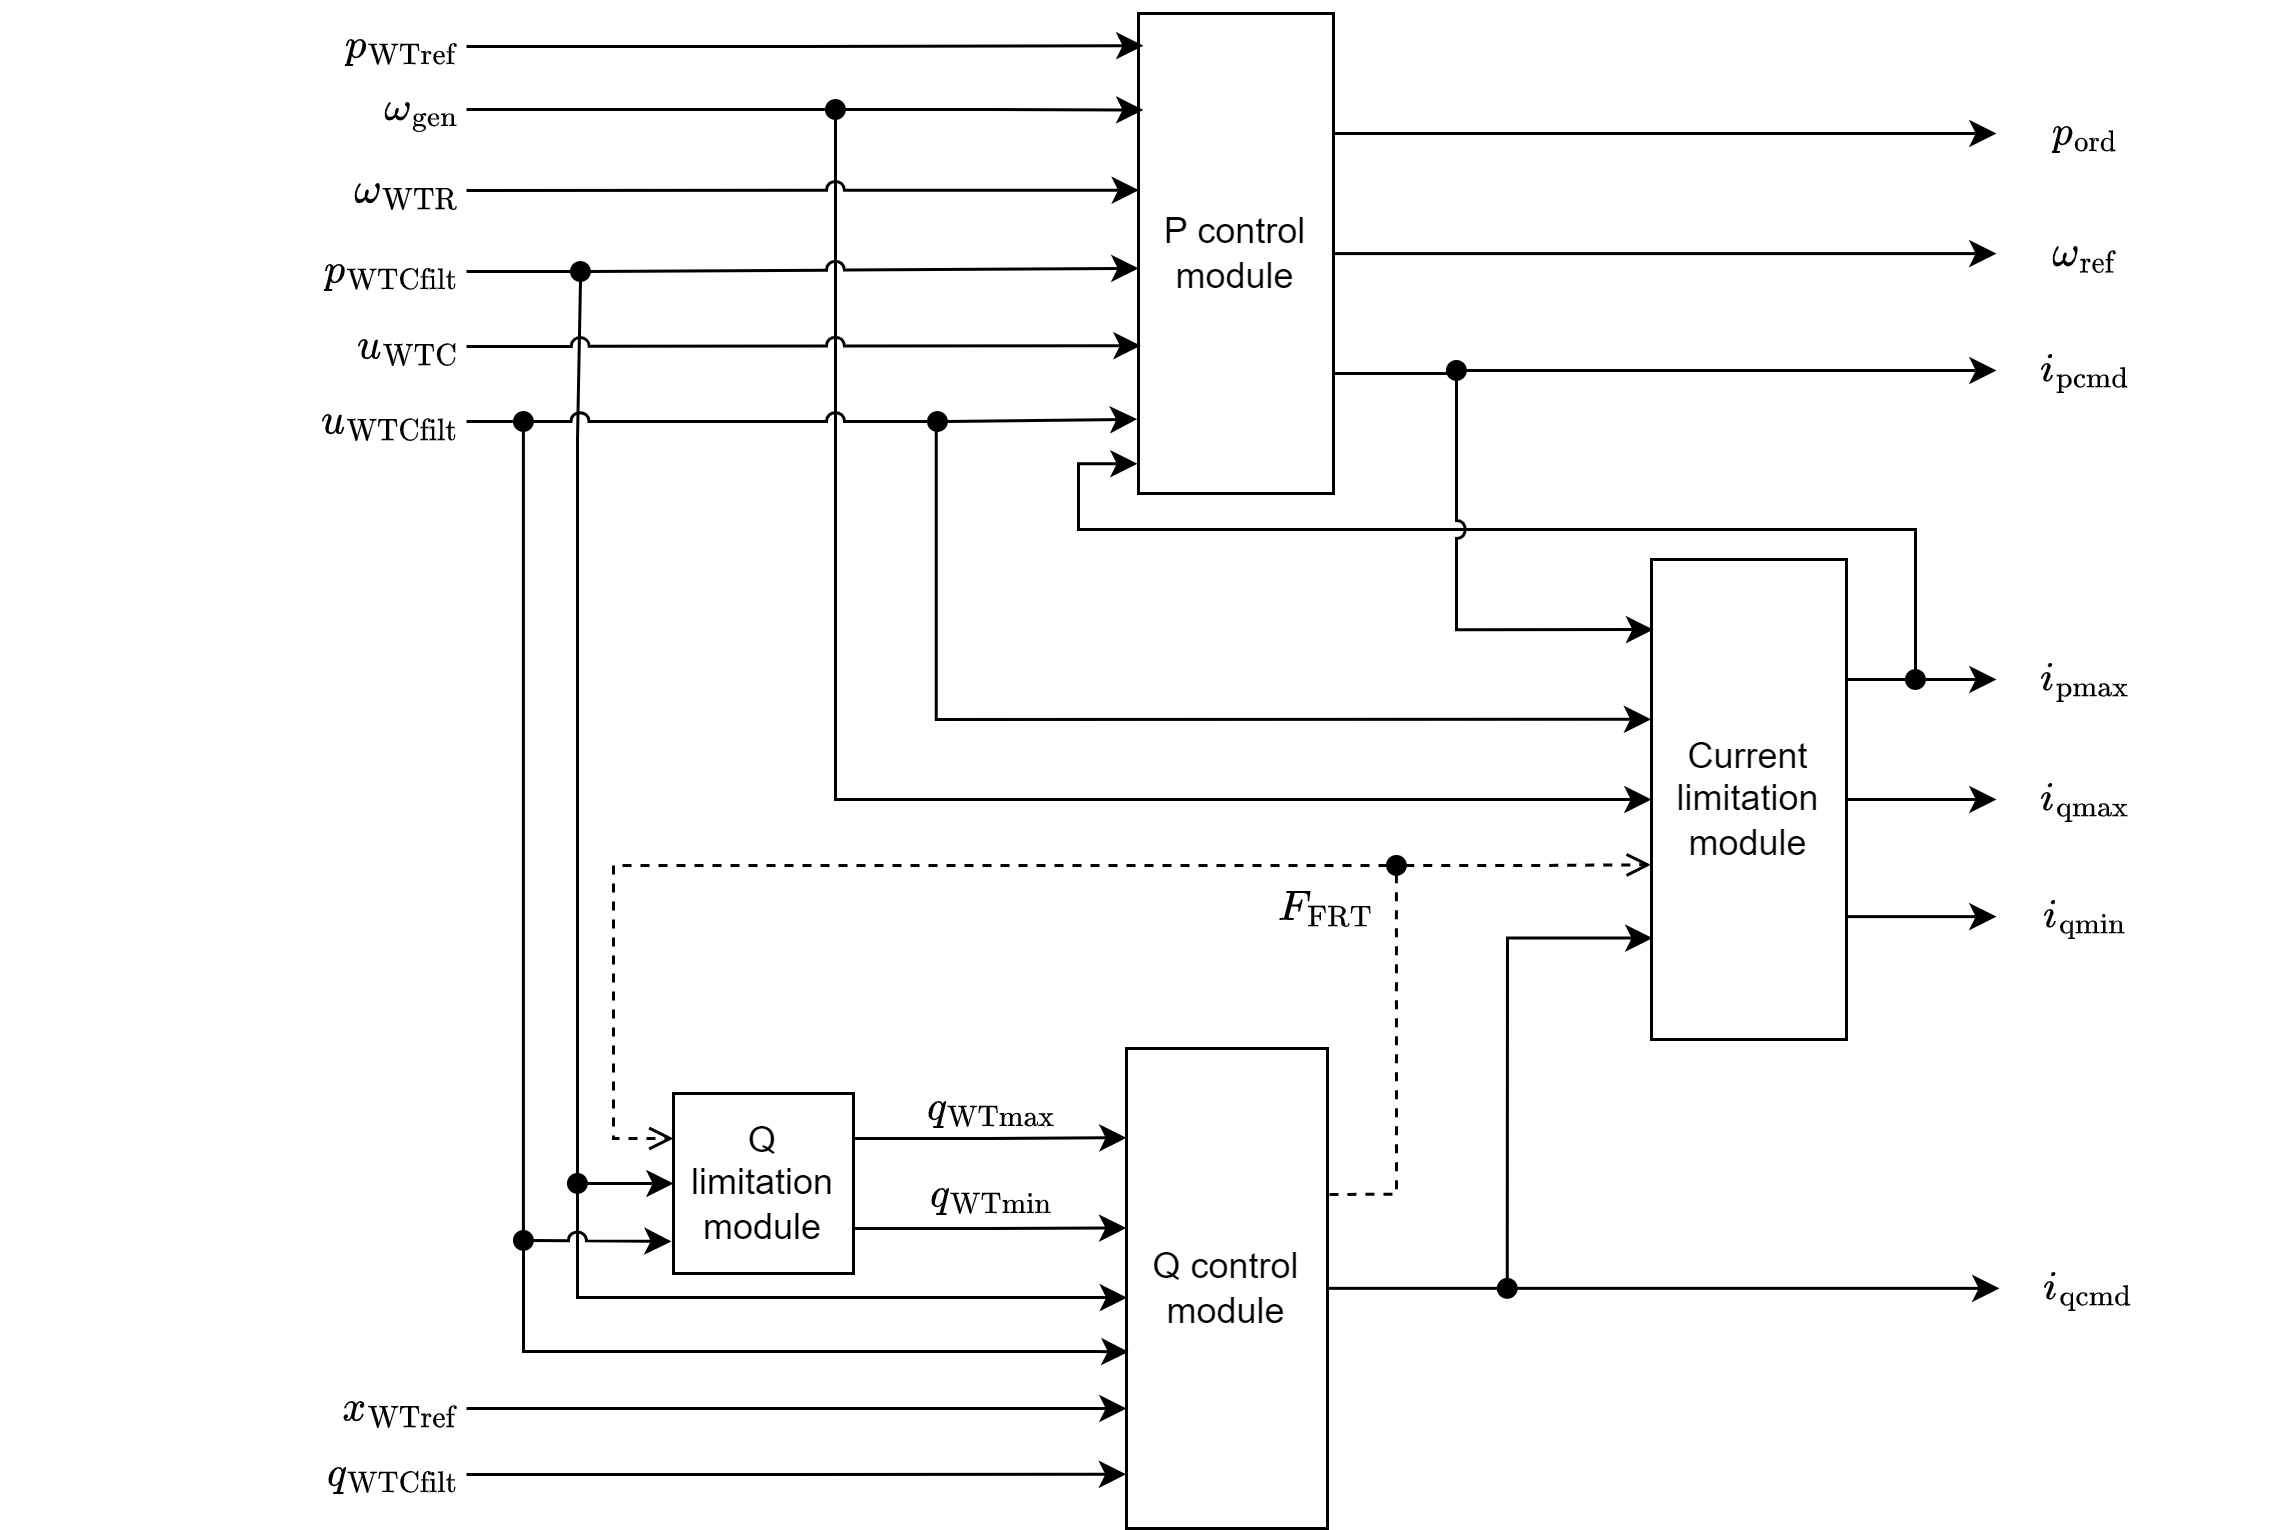
\includegraphics{drawings/WT_generator_control_substructure_type3.drawio.png}

}

\caption{\label{fig-wtControlSubstructure}Wind turbine generator control
sub-structure for Type 3A and 3B WT, based on {[}1{]}}

\end{figure}%

\subsection{P control module}\label{sec-wt-p-control}

For detailed assessment of the parameters' impact on model behaviour,
see {[}5{]}.

\begin{figure}

\centering{

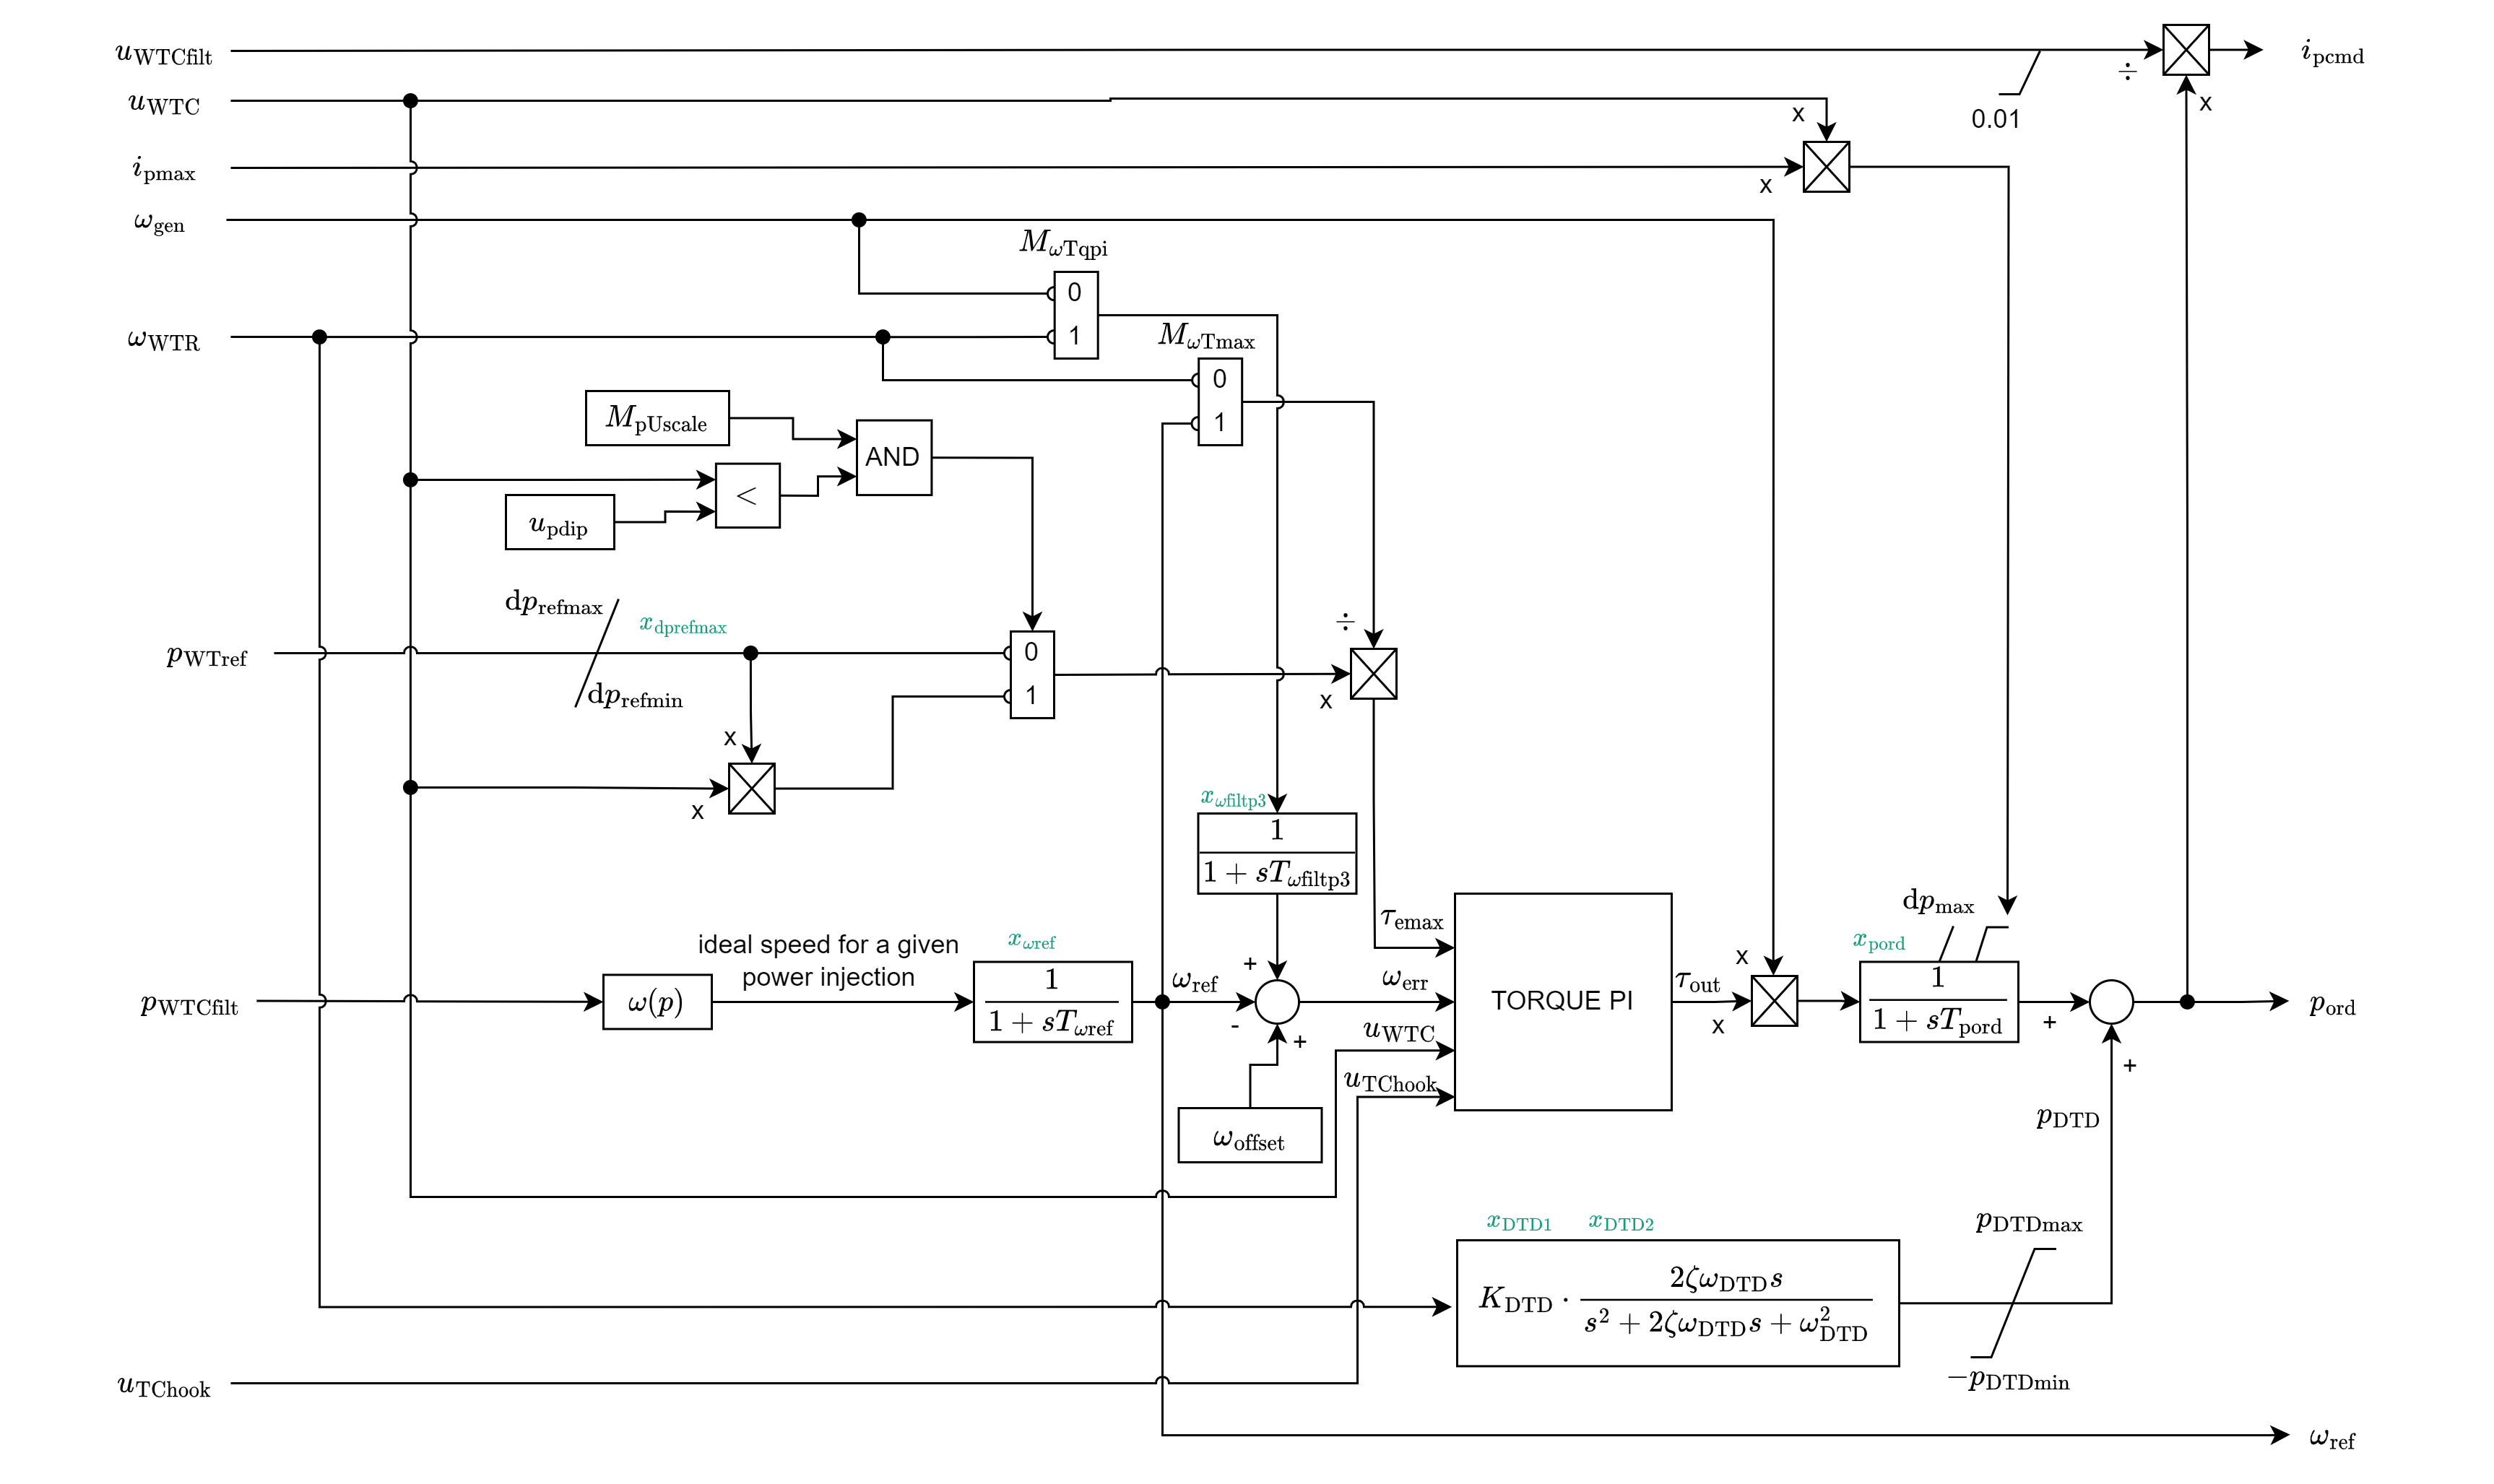
\includegraphics{drawings/WT_P_control_type3.drawio.png}

}

\caption{\label{fig-wtPControl}Wind turbine P control module (Type 3),
based on {[}1{]}}

\end{figure}%

Figure~\ref{fig-wtPControl} shows the wind turbine active power control
scheme.

The control's general behaviour is dominated by \(\omega(p)\), a
lookup-table that provides the angular velocity at which the turbine
should rotate when it is injecting a certain active power {[}6{]}. A
possible look-up table for this system is shown in
Figure~\ref{fig-lookup-table-omega-pref}, which is representing example
values from \emph{DIgSILENT PowerFactory}.

The power-speed-characteristic in
Figure~\ref{fig-lookup-table-omega-pref} has four main operating zones
according to {[}5{]}:

\begin{itemize}
\tightlist
\item
  \textbf{Zone 1:} The minimum rotational speed has been reached and
  hence cannot decrease further due to physical (component) limits,
  mainly maximum slip of the converter.
\item
  \textbf{Zone 2:} Between minimum rotational speed to rated rotational
  speed; maximum power tracking mode.
\item
  \textbf{Zone 3:} Fixed at rated speed and below the rated active
  power. In some cases, instead of a fixed rated rotational speed, there
  is a linear rotational speed variation to achieve the rated rotational
  speed at the rated active power.
\item
  \textbf{Zone 4:} Rated rotational speed and rated active power.
\end{itemize}

\begin{tcolorbox}[enhanced jigsaw, coltitle=black, bottomrule=.15mm, opacitybacktitle=0.6, rightrule=.15mm, colframe=quarto-callout-note-color-frame, titlerule=0mm, arc=.35mm, breakable, colbacktitle=quarto-callout-note-color!10!white, title=\textcolor{quarto-callout-note-color}{\faInfo}\hspace{0.5em}{Note}, colback=white, bottomtitle=1mm, toprule=.15mm, leftrule=.75mm, toptitle=1mm, left=2mm, opacityback=0]

Dotted lines in Figure~\ref{fig-lookup-table-omega-pref} imply that, for
simulations, the active power reference presents a certain slope,
offering more stable simulations. Under real control conditions, this
look-up table has two vertical lines, as shown by the solid lines.
{[}5{]}

\end{tcolorbox}

\begin{Shaded}
\begin{Highlighting}[]
\ImportTok{from}\NormalTok{ matplotlib }\ImportTok{import}\NormalTok{ pyplot }\ImportTok{as}\NormalTok{ plt}
\ImportTok{import}\NormalTok{ seaborn }\ImportTok{as}\NormalTok{ sns}
\NormalTok{colors }\OperatorTok{=}\NormalTok{ sns.color\_palette(}\StringTok{\textquotesingle{}Set2\textquotesingle{}}\NormalTok{)}
\NormalTok{sns.set\_palette(colors)}

\NormalTok{plt.plot(}
\NormalTok{    [}\FloatTok{0.755}\NormalTok{,  }\FloatTok{0.76}\NormalTok{,   }\FloatTok{0.86}\NormalTok{,   }\FloatTok{0.94}\NormalTok{,   }\DecValTok{1}\NormalTok{,      }\FloatTok{1.01}\NormalTok{], }
\NormalTok{    [}\DecValTok{0}\NormalTok{,      }\FloatTok{0.3}\NormalTok{,    }\FloatTok{0.31}\NormalTok{,   }\FloatTok{0.4}\NormalTok{,    }\FloatTok{0.5}\NormalTok{,    }\DecValTok{1}\NormalTok{], }
    \StringTok{\textquotesingle{}{-}{-}\textquotesingle{}}\NormalTok{, c}\OperatorTok{=}\NormalTok{colors[}\DecValTok{0}\NormalTok{])}
\NormalTok{plt.plot(}
\NormalTok{    [}\FloatTok{0.76}\NormalTok{,  }\FloatTok{0.76}\NormalTok{,   }\FloatTok{0.86}\NormalTok{,   }\FloatTok{0.94}\NormalTok{,   }\DecValTok{1}\NormalTok{,      }\DecValTok{1}\NormalTok{], }
\NormalTok{    [}\DecValTok{0}\NormalTok{,     }\FloatTok{0.3}\NormalTok{,    }\FloatTok{0.31}\NormalTok{,   }\FloatTok{0.4}\NormalTok{,    }\FloatTok{0.5}\NormalTok{,    }\DecValTok{1}\NormalTok{], }
    \StringTok{\textquotesingle{}{-}x\textquotesingle{}}\NormalTok{, c}\OperatorTok{=}\NormalTok{colors[}\DecValTok{0}\NormalTok{])}
\NormalTok{plt.grid()}
\NormalTok{\_ }\OperatorTok{=}\NormalTok{ plt.ylabel(}\VerbatimStringTok{r\textquotesingle{}$p\_\textbackslash{}mathrm}\SpecialCharTok{\{WT\}}\VerbatimStringTok{$ in pu\textquotesingle{}}\NormalTok{)}
\NormalTok{\_ }\OperatorTok{=}\NormalTok{ plt.xlabel(}\VerbatimStringTok{r\textquotesingle{}$\textbackslash{}omega\_\textbackslash{}mathrm}\SpecialCharTok{\{ref\}}\VerbatimStringTok{$ in pu\textquotesingle{}}\NormalTok{)}
\NormalTok{plt.xlim(}\FloatTok{0.7}\NormalTok{,}\FloatTok{1.1}\NormalTok{)}
\NormalTok{\_ }\OperatorTok{=}\NormalTok{ plt.text(}\FloatTok{1.03}\NormalTok{, }\FloatTok{.99}\NormalTok{, }\StringTok{\textquotesingle{}Zone 4\textquotesingle{}}\NormalTok{, ha}\OperatorTok{=}\StringTok{\textquotesingle{}left\textquotesingle{}}\NormalTok{, va}\OperatorTok{=}\StringTok{\textquotesingle{}top\textquotesingle{}}\NormalTok{)}
\NormalTok{\_ }\OperatorTok{=}\NormalTok{ plt.text(}\FloatTok{.99}\NormalTok{, }\FloatTok{.8}\NormalTok{, }\StringTok{\textquotesingle{}Zone 3\textquotesingle{}}\NormalTok{, ha}\OperatorTok{=}\StringTok{\textquotesingle{}right\textquotesingle{}}\NormalTok{, va}\OperatorTok{=}\StringTok{\textquotesingle{}top\textquotesingle{}}\NormalTok{)}
\NormalTok{\_ }\OperatorTok{=}\NormalTok{ plt.text(}\FloatTok{.9}\NormalTok{, }\FloatTok{.45}\NormalTok{, }\StringTok{\textquotesingle{}Zone 2\textquotesingle{}}\NormalTok{, ha}\OperatorTok{=}\StringTok{\textquotesingle{}right\textquotesingle{}}\NormalTok{, va}\OperatorTok{=}\StringTok{\textquotesingle{}top\textquotesingle{}}\NormalTok{)}
\NormalTok{\_ }\OperatorTok{=}\NormalTok{ plt.text(}\FloatTok{.745}\NormalTok{, }\FloatTok{.1}\NormalTok{, }\StringTok{\textquotesingle{}Zone 1\textquotesingle{}}\NormalTok{, ha}\OperatorTok{=}\StringTok{\textquotesingle{}right\textquotesingle{}}\NormalTok{, va}\OperatorTok{=}\StringTok{\textquotesingle{}top\textquotesingle{}}\NormalTok{)}
\end{Highlighting}
\end{Shaded}

\begin{figure}[H]

\centering{

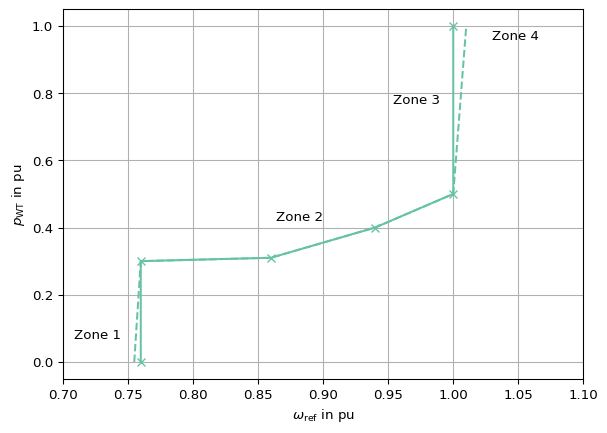
\includegraphics{WindType3_files/figure-pdf/fig-lookup-table-omega-pref-output-1.pdf}

}

\caption{\label{fig-lookup-table-omega-pref}Lookup table for reference
rotation speed as a function of WT active power; according to {[}5{]}
and with data from \emph{DIgSILENT PowerFactory} (see
Table~\ref{tbl-wtLookupTable})}

\end{figure}%

The power-speed-characteristic's speed reference output is then filtered
(\(T_\mathrm{\omega ref}\)) to avoid sudden changes.

\begin{tcolorbox}[enhanced jigsaw, coltitle=black, bottomrule=.15mm, opacitybacktitle=0.6, rightrule=.15mm, colframe=quarto-callout-note-color-frame, titlerule=0mm, arc=.35mm, breakable, colbacktitle=quarto-callout-note-color!10!white, title=\textcolor{quarto-callout-note-color}{\faInfo}\hspace{0.5em}{Note}, colback=white, bottomtitle=1mm, toprule=.15mm, leftrule=.75mm, toptitle=1mm, left=2mm, opacityback=0]

The time constant \(T_\mathrm{\omega ref}\) can be set to a very high
value to enforce a fixed reference rotational speed during the
simulation, which can be a desired operational mode. {[}5{]}

\end{tcolorbox}

The filtered speed reference \(\omega_\mathrm{ref}\) is subtracted from
the measured angular velocity \(\omega_\text{gen}\) (generator speed) or
\(\omega_\mathrm{WTR}\) (turbine speed), depending on the mode
\(M_\mathrm{\omega Tqpi}\) to get the speed error
\(\omega_\mathrm{err}\). The measured speed can be filtered by the first
order lag element with time constant \(T_\mathrm{\omega filtp3}\).

Since \(\omega_\mathrm{gen}\) comes from the mechanical module which
only models the drive train resonant frequency, this first order lag is
intended as a filter for only this oscillation. Since it is a low pass,
it won't be able to efficiently filter that resonance from the signal.
Alternatively, by setting \(M_\mathrm{\omega Tqpi}=\mathrm{true}\), the
rotor speed \(\omega_\mathrm{WTR}\) can be used instead of the generator
speed, which acts as a simpler way to determine a filtered value of
\(\omega_\mathrm{gen}\) {[}5{]}.

The speed error \(\omega_\mathrm{err}\) is then given to the
\emph{Torque PI controller} (Figure~\ref{fig-torquePi}), which outputs
the electromagnetic torque reference \(\tau_\mathrm{out}\) {[}6{]}.

Another input to the torque PI subsystem (see
Section~\ref{sec-torque-pi}) is the maximum electromagnetic torque
\(\tau_\mathrm{emax}\). It is determined by calculating a torque value
from {[}5{]}:

\begin{itemize}
\tightlist
\item
  The reference power value \(p_\mathrm{WTref}\), during voltage dips
  optionally scaled down by the terminal voltage \(u_\mathrm{WTC}\) (if
  \(M_\mathrm{pUscale}=\mathrm{true}\))
\item
  And a rotational speed, either the turbine rotor speed
  \(\omega_\mathrm{WTR}\) (if \(M_\mathrm{\omega Tmax}=\mathrm{false}\))
  or the speed reference value \(\omega_\mathrm{ref}\) (if
  \(M_\mathrm{\omega Tmax}=\mathrm{true}\)).
\end{itemize}

After the torque PI controller, the electromagnetic torque reference
\(\tau_\mathrm{out}\) is multiplied by the generator's rotational speed
\(\omega_\mathrm{gen}\) to obtain a power reference {[}6{]}.

To obtain the active current command \(i_\mathrm{pcmd}\),
\(p_\mathrm{ord}\) is divided by the measured voltage
\(u_\mathrm{WTCfilt}\).

To the active power order \(p_\mathrm{ord}\) an additional component
from the Drive Train Damping (DTD) system is added. Physically, the DTD
provides an electrical torque that accounts for natural damping by
considering speed differences between both low and high speed shafts
(either side of the gearbox) {[}5{]}. It is modeled through a
second-order transfer function as shown towards the bottom right of
Figure~\ref{fig-wtPControl}:

\[
K_{\text{DTD}} \cdot \frac{2 \zeta \omega_{\text{DTD}} s}{s^2 + 2 \zeta \omega_{\text{DTD}} s + \omega_{\text{DTD}}^2}
\]

As mentioned above, in this model the DTD is represented by an active
power component, not a torque. The transfer function outputs an
oscillating electrical power that has an efficient damping effect
{[}5{]} (for parameters see Section~\ref{sec-wt-p-params}).

\subsubsection{Torque PI block}\label{sec-torque-pi}

\begin{figure}

\centering{

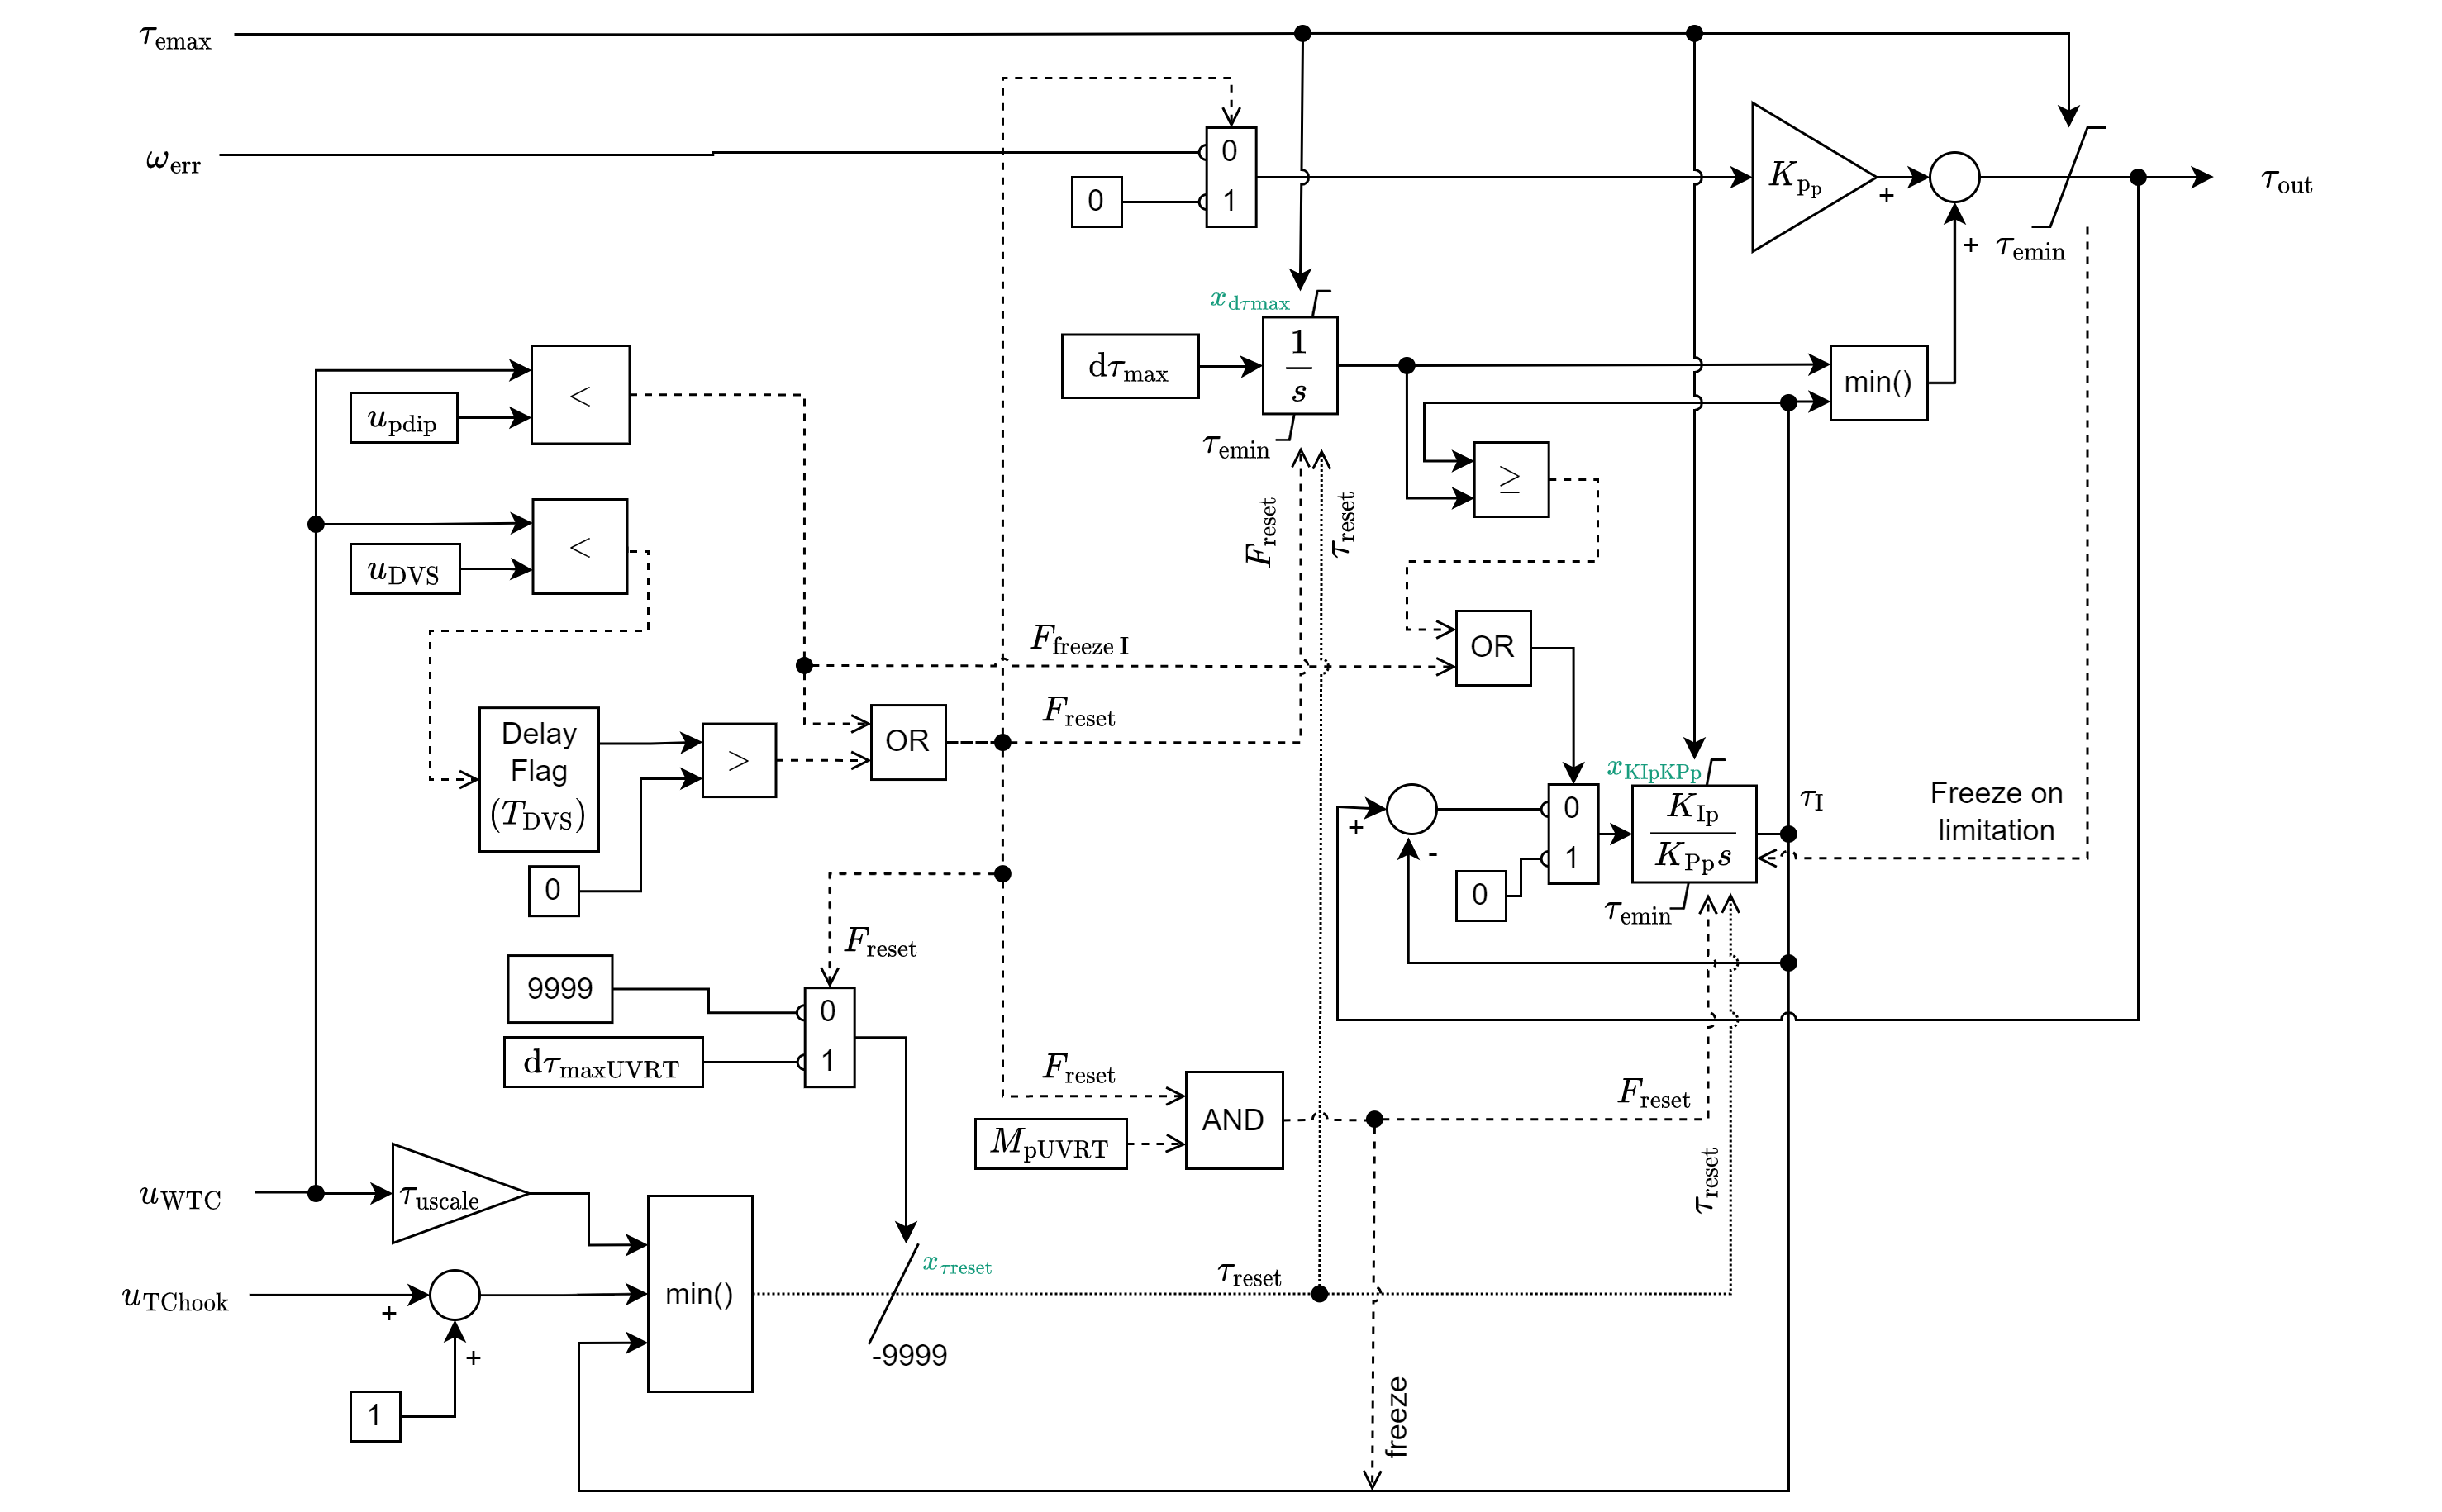
\includegraphics{drawings/WT_torque_pi.drawio.png}

}

\caption{\label{fig-torquePi}Wind turbine torque PI block (Type 3),
based on {[}1{]}}

\end{figure}%

In Figure~\ref{fig-torquePi} the Torque PI Block can be seen. It it acts
as a PI-controller and is a subsystem of the active power control in
Figure~\ref{fig-wtPControl} {[}6{]}.

For the calculation of the speed error input \(\omega_\mathrm{err}\) and
the maximum electromagnetic torque input \(\tau_\mathrm{emax}\), see
Section~\ref{sec-wt-p-control}.

\textbf{Proportional and integral parts of the controller}

The proportional controller part is realized by \(K_\mathrm{Pp}\).

The integral part of the controller output is the smaller of the
following two signals {[}6{]}:

\begin{itemize}
\tightlist
\item
  The output of the integral controller \(K_\mathrm{Ip}/K_\mathrm{Pp}\)
\item
  A torque value increasing as a ramp with rising rate
  \(\mathrm{d}\tau_\mathrm{max}\), which can be used to control the
  mechanical stress or to meet grid code requirements. This is set to
  \(\tau_\mathrm{reset}\) when a low voltage fault occurs and ramps
  upwards after the fault.
\end{itemize}

\textbf{Behavior during low voltage faults}

The \emph{Delay Flag} block takes a boolean value \(F_\mathrm{i}\) as
input. If \(F_\mathrm{i}\) steps to 1, the integer output
\(F_\mathrm{o}\) is 1 and a \emph{timer} starts to run. As soon as
\(F_\mathrm{i}\) steps back to 0, \(F_\mathrm{o}\) steps to 2 if the
\emph{timer} has not reached \(T_\mathrm{DVS}\). Once the timer reaches
\(T_\mathrm{DVS}\), \(F_\mathrm{o}\) steps back to 0. {[}1{]}

The delay flag block is used to implement the following fault signals:

\begin{itemize}
\tightlist
\item
  \(F_\mathrm{reset}\) is true during a volage dip
  (\(u_\mathrm{WTC} < u_\mathrm{pdip}\)) as well as during and
  \(T_\mathrm{DVS}\) after a deep voltage dip
  (\(u_\mathrm{WTC} < u_\mathrm{DVS}\)).
\item
  \(F_\mathrm{freeze\,I}\) is true during a voltage dip
  (\(u_\mathrm{WTC} < u_\mathrm{pdip}\))
\end{itemize}

These fault signals have the following functions:

\begin{itemize}
\tightlist
\item
  \(F_\mathrm{reset}\), while true,

  \begin{itemize}
  \tightlist
  \item
    resets and holds both integrators at \(\tau_\mathrm{reset}\) (see
    below); for the \(K_\mathrm{Ip}/K_\mathrm{Pp}\)-integrator this can
    be prevented by setting \(M_\mathrm{pUVRT} = \mathrm{false}\).
  \item
    sets the speed error \(\omega_\mathrm{err}\), i.e.~the input to the
    proportional controller part \(K_\mathrm{Pp}\), to zero
  \item
    changes the upper ramp rate limit of \(\tau_\mathrm{reset}\) to
    \(\mathrm{d}\tau_\mathrm{maxUVRT}\) (usually set to zero, preventing
    \(\tau_\mathrm{reset}\) from inceasing during fault) {[}6{]}
  \end{itemize}
\item
  \(F_\mathrm{freeze\,I}\) freezes the integral controller part
  (\(K_\mathrm{Ip}/K_\mathrm{Pp}\)) while true.
\end{itemize}

The reset value \(\tau_\mathrm{reset}\) is the minimum value of:

\begin{itemize}
\tightlist
\item
  The measured voltage (during fault) multiplied by factor
  \(\tau_\mathrm{uscale}\)
\item
  The output \(\tau_\mathrm{I}\) of the integrator itself
\item
  \(u_\mathrm{TChook} + 1\)
\end{itemize}

\(\tau_\mathrm{uscale}\) can be used to alter the power injection
behaviour during fault and also the starting point for power recovery
after post-fault. For example, setting it to zero results in zero power
injection during fault. Higher values increase power injection, until
the current limitation system begins to limit. See {[}6{]} for further
details.

When \(F_\mathrm{reset}\) returns to false, the proportional controller
\(K_\mathrm{Pp}\) will work again as before the fault. The integral
controller will increase from \(\tau_\mathrm{reset}\) to steady-state,
with a maximum rate dictated by \(\mathrm{d}\tau_\mathrm{max}\) {[}6{]}.

\subsubsection{Variable limits integrator with set/reset and
freeze}\label{variable-limits-integrator-with-setreset-and-freeze}

The integrators used in the Torque PI model in Figure~\ref{fig-torquePi}
need variable limits, set/reset and freeze functionalities. A suggestion
for the implementation is shown below and the description follows
thereafter.

\begin{Shaded}
\begin{Highlighting}[]
\NormalTok{model IntegratorVariableLimitsContinuousSetFreeze "Integrator with limited value of output (variable limits), set/reset and freeze"}
\NormalTok{    parameter Boolean DefaultLimitMax = true "If limitMin \textgreater{} limitMax : if true, y = limitMax, if false, y = limitMin";}
\NormalTok{    parameter Real K = 1 "Integrator gain";}
\NormalTok{    parameter Real LimitMax0 "Initial value of upper limit";}
\NormalTok{    parameter Real LimitMin0 "Initial value of lower limit";}
\NormalTok{    parameter Boolean ReinitWhenResetIsReleased = true "true: integrator state gets reinitialized to \textquotesingle{}set\textquotesingle{} when \textquotesingle{}reset\textquotesingle{} turns false. false: integrator state gets reinitialized to \textquotesingle{}set\textquotesingle{} when \textquotesingle{}reset\textquotesingle{} turns true.";}
\NormalTok{    parameter Real tDer = 1e{-}3 "Time constant of derivative filter for limits in s";}
\NormalTok{    parameter Real TolInput = 1e{-}5 "Tolerance on limit crossing for integrator input";}
\NormalTok{    parameter Real TolOutput = 1e{-}5 "Tolerance on limit crossing for integrator output";}
\NormalTok{    parameter Real LimitDeadband = 0.001 "Deadband for detecting a limit crossing of the integrator\textquotesingle{}s state";}
\NormalTok{    Real w(start = Y0) "Integrator state variable";}
\NormalTok{    parameter Real Y0 = 0 "Initial or guess value of output (must be in the limits limitMin .. limitMax)";}

\NormalTok{    Real kFreezeMax "Freeze coefficient for upper limit";}
\NormalTok{    Real kFreezeMin "Freeze coefficient for lower limit";}
\NormalTok{    Real derLimitMax "Filtered derivative of upper limit of output";}
\NormalTok{    Real derLimitMin "Filtered derivative of lower limit of output";}
\NormalTok{    Modelica.Blocks.Interfaces.BooleanInput freeze "Optional connector of freeze signal";}
\NormalTok{    Modelica.Blocks.Interfaces.RealInput limitMax "Connector of Real input signal used as maximum of output y";}
\NormalTok{    Modelica.Blocks.Interfaces.RealInput limitMin "Connector of Real input signal used as minimum of output y";}
\NormalTok{    Modelica.Blocks.Interfaces.BooleanInput reset "Optional connector of reset signal";}
\NormalTok{    Modelica.Blocks.Interfaces.RealInput set "Optional connector of set signal";}
\NormalTok{equation}
    
\NormalTok{    ////////// reset or freeze: keep input = 0}
\NormalTok{    if freeze or reset then}
\NormalTok{        v = 0;}
\NormalTok{    else}
\NormalTok{        v = K * u;}
\NormalTok{    end if;}
    
\NormalTok{    ////////// reset: reinit integrator\textquotesingle{}s state when set becomes false (or true, depending on ReinitWhenResetIsReleases)}
\NormalTok{    when if ReinitWhenResetIsReleased then not reset else reset then}
\NormalTok{      reinit(w, set);}
\NormalTok{    end when;}
    
\NormalTok{    ////////// integrator with limits}
\NormalTok{    derLimitMax = der(limitMax);}
\NormalTok{    derLimitMin = der(limitMin);}
\NormalTok{    kFreezeMax = 1 / 4 * (1 + tanh((w {-} limitMax) / TolOutput)) * (1 + tanh((v {-} derLimitMax) / TolInput));}
\NormalTok{    kFreezeMin = 1 / 4 * (1 + tanh((limitMin {-} w) / TolOutput)) * (1 + tanh((derLimitMin {-} v) / TolInput));}
\NormalTok{    der(w) = derLimitMax * kFreezeMax + derLimitMin * kFreezeMin + v * (1 {-} kFreezeMax {-} kFreezeMin);}
    
\NormalTok{    ////////// apply limit or set to output}
\NormalTok{    if limitMin \textgreater{} limitMax and DefaultLimitMax then}
\NormalTok{        y = limitMax;}
\NormalTok{    elseif limitMin \textgreater{} limitMax then}
\NormalTok{        y = limitMin;}
\NormalTok{    elseif w \textgreater{} limitMax+LimitDeadband then}
\NormalTok{        y = limitMax;}
\NormalTok{    elseif w \textless{} limitMin{-}LimitDeadband then}
\NormalTok{        y = limitMin;}
\NormalTok{    elseif reset then}
\NormalTok{        y = set;}
\NormalTok{    else}
\NormalTok{        y = w;}
\NormalTok{    end if;}
\NormalTok{end IntegratorVariableLimitsContinuousSetFreeze;}
\end{Highlighting}
\end{Shaded}

This blocks computes \texttt{w} as integral of the input \texttt{u}
multiplied by the gain \texttt{K}, with \texttt{v\ =\ K\ *\ u}. If the
integral reaches a given upper limit limitMax or lower limit limitMin,
the integration is halted and only restarted if the input drives the
integral away from the bounds.

This freeze is imposed through two coefficients \texttt{kFreezeMax} and
\texttt{kFreezeMin}, each defined by a continuous expression involving
the hyperbolic tangent, the integrator input \texttt{v}, the integrator
output \texttt{w}, the limit \texttt{limitMax} or \texttt{limitMin} and
its filtered derivative \texttt{derLimitMax} or \texttt{derLimitMin}.

The parameters \texttt{TolInput} and \texttt{TolOutput} determine the
width of the transition zone from one domain to another.

The output \texttt{y} is the result of the limitation of \texttt{w} by
both variable limits.

If the ``upper'' limit is smaller than the ``lower'' one, the output
\texttt{y} is ruled by the parameter \texttt{DefaultLimitMax}:
\texttt{y} is equal to either \texttt{limitMax} or \texttt{limitMin}.

\textbf{set/reset}

The integrator's output is forced to the value of \texttt{set} while
\texttt{reset=true}, as it is descibed in {[}1{]}.

When \texttt{reset} returns to false (=falling edge), the integrator's
state is reinitialized to set to resume integration without a jump
discontinuity (change \texttt{ReinitWhenResetIsReleased} to
\texttt{false} to reinitialize at a rising edge instead).

\textbf{freeze}

If boolean input is set to true, the derivative of the state variable is
set to zero.

\subsubsection{Parameters}\label{sec-wt-p-params}

Typical values were gathered from the \emph{DIgSILENT PowerFactory}
implementation of the model.

\begin{longtable}[]{@{}
  >{\raggedright\arraybackslash}p{(\columnwidth - 12\tabcolsep) * \real{0.0800}}
  >{\raggedright\arraybackslash}p{(\columnwidth - 12\tabcolsep) * \real{0.0600}}
  >{\raggedright\arraybackslash}p{(\columnwidth - 12\tabcolsep) * \real{0.0500}}
  >{\raggedright\arraybackslash}p{(\columnwidth - 12\tabcolsep) * \real{0.1600}}
  >{\raggedright\arraybackslash}p{(\columnwidth - 12\tabcolsep) * \real{0.2000}}
  >{\raggedright\arraybackslash}p{(\columnwidth - 12\tabcolsep) * \real{0.3500}}
  >{\raggedright\arraybackslash}p{(\columnwidth - 12\tabcolsep) * \real{0.0700}}@{}}
\caption{Parameters, based on {[}1{]}, {[}5{]} and \emph{DIgSILENT
PowerFactory}}\label{tbl-parameters}\tabularnewline
\toprule\noalign{}
\begin{minipage}[b]{\linewidth}\raggedright
name
\end{minipage} & \begin{minipage}[b]{\linewidth}\raggedright
type
\end{minipage} & \begin{minipage}[b]{\linewidth}\raggedright
unit
\end{minipage} & \begin{minipage}[b]{\linewidth}\raggedright
base
\end{minipage} & \begin{minipage}[b]{\linewidth}\raggedright
modelica name
\end{minipage} & \begin{minipage}[b]{\linewidth}\raggedright
description
\end{minipage} & \begin{minipage}[b]{\linewidth}\raggedright
typical value
\end{minipage} \\
\midrule\noalign{}
\endfirsthead
\toprule\noalign{}
\begin{minipage}[b]{\linewidth}\raggedright
name
\end{minipage} & \begin{minipage}[b]{\linewidth}\raggedright
type
\end{minipage} & \begin{minipage}[b]{\linewidth}\raggedright
unit
\end{minipage} & \begin{minipage}[b]{\linewidth}\raggedright
base
\end{minipage} & \begin{minipage}[b]{\linewidth}\raggedright
modelica name
\end{minipage} & \begin{minipage}[b]{\linewidth}\raggedright
description
\end{minipage} & \begin{minipage}[b]{\linewidth}\raggedright
typical value
\end{minipage} \\
\midrule\noalign{}
\endhead
\bottomrule\noalign{}
\endlastfoot
\(\mathrm{d}p_{\mathrm{max}}\) & float & pu &
\(S_{\mathrm{base}} / \mathrm{s}\) & DPMaxPu & Maximum ramp rate of wind
turbine power & 999 \\
\(\mathrm{d}p_{\mathrm{refmax}}\) & float & pu &
\(S_{\mathrm{base}} / \mathrm{s}\) & DPRefMaxPu & Maximum ramp rate for
reference power of the wind turbine & 0.3 \\
\(\mathrm{d}p_{\mathrm{refmin}}\) & float & pu &
\(S_{\mathrm{base}} / \mathrm{s}\) & DPRefMinPu & Minimum ramp rate for
reference power of the wind turbine & -0.3 \\
\(\mathrm{d}\tau_{\mathrm{max}}\) & float & pu &
\(T_{\mathrm{base}} / \mathrm{s}\) & DTauMaxPu & Torque ramp rate limit,
as required by some grid codes & 0.25 \\
\(\mathrm{d}\tau_{\mathrm{maxUVRT}}\) & float & pu &
\(T_{\mathrm{base}} / \mathrm{s}\) & DTauUvrtMaxPu & Torque rise rate
limit during UVRT & 0 \\
\(K_{\mathrm{DTD}}\) & float & pu &
\(S_{\mathrm{base}} / \Omega_{\mathrm{base}}\) & KDtd & Active drive
train damping: gain & 1.5 (or 0 if
\(M_\mathrm{\omega Tqpi}=\mathrm{false}\)) {[}5{]} \\
\(K_{\mathrm{Ip}}\) & float & pu &
\(T_{\mathrm{base}} / \Omega_{\mathrm{base}} / \mathrm{s}\) & KIp &
Integrator time constant of the PI controller & 5 \\
\(K_{\mathrm{Pp}}\) & float & pu &
\(T_{\mathrm{base}} / \Omega_{\mathrm{base}}\) & KPp & Proportional gain
of the PI controller & 8 \\
\(M_\mathrm{\omega Tmax}\) & bool & - & - & MOmegaTMax & Mode for source
of rotational speed for maximum torque calculation
\((false: \omega_{\mathrm{WTR}} - true: \omega_{\mathrm{ref}})\) &
true \\
\(M_\mathrm{\omega Tqpi}\) & bool & - & - & MOmegaTqpi & Mode for source
of rotational speed for torque PI controller error calculation
\((false: \omega_{\mathrm{gen}} - true: \omega_{\mathrm{WTR}})\) & true
(or false if \(K_\mathrm{DTD}=0\)) {[}5{]} \\
\(M_{\mathrm{pUscale}}\) & bool & - & - & MPUscale & Enable voltage
scaling for power reference during a voltage dip (false: no scaling --
true: u scaling) & false \\
\(M_{\mathrm{pUVRT}}\) & bool & - & - & MPUvrt & Mode for UVRT power
control (false: reactive power control -- true: voltage control) &
true \\
\(\omega_{\mathrm{DTD}}\) & float & pu & \(\Omega_{\mathrm{base}}\) &
OmegaDtdPu & Active drive train damping: frequency, derived from
two-mass model parameters, see Equation~\ref{eq-omegaDtd} & 11.3 \\
\(\omega_{\mathrm{offset}}\) & float & pu & \(\Omega_{\mathrm{base}}\) &
OmegaOffsetPu & Offset from the reference value to limit controller
action during rotor speed changes & 0 \\
\(\omega(p)\) & float & pu &
\(\Omega_{\mathrm{base}}(S_{\mathrm{base}})\) & TableOmegaPPu & Lookup
table for power as a function of speed & see
Table~\ref{tbl-wtLookupTable} \\
\(p_{\mathrm{DTDmax}}\) & float & pu & \(S_{\mathrm{base}}\) & PDtdMaxPu
& Active drive train damping: maximum power & 0.15 \\
\(\tau_{\mathrm{emin}}\) & float & pu & \(T_{\mathrm{base}}\) &
TauEMinPu & Minimum torque for the electrical generator & 0.001 \\
\(\tau_{\mathrm{uscale}}\) & float & pu &
\(T_{\mathrm{base}} / U_{\mathrm{base}}\) & TauUscalePu & Voltage
scaling factor for reset torque & 1 \\
\(T_{\mathrm{DVS}}\) & float & s & - & tDvs & Time delay following deep
a voltage dip & 0.05 \\
\(T_{\mathrm{\omega filtp3}}\) & float & s & - & tOmegafiltp3 & Filter
time constant for measuring generator speed & 0.005 \\
\(T_{\mathrm{\omega ref}}\) & float & s & - & tOmegaRef & Time constant
in the speed reference filter & 0.005 \\
\(T_{\mathrm{pord}}\) & float & s & - & tPord & Power order lag time
constant & 0.01 \\
\(u_{\mathrm{DVS}}\) & float & pu & \(U_{\mathrm{base}}\) & UDvsPu &
Voltage limit for maintaining UVRT status after a deep voltage dip &
0.15 \\
\(u_{\mathrm{pdip}}\) & float & pu & \(U_{\mathrm{base}}\) & UPdipPu &
Voltage dip threshold for active power control, often different from
converter thresholds (e.g., 0.8) & 0.9 \\
\(\zeta\) & float & pu & - & Zeta & Active drive train damping: damping
coefficient & 0.5 \\
\end{longtable}

\begin{tcolorbox}[enhanced jigsaw, coltitle=black, bottomrule=.15mm, opacitybacktitle=0.6, rightrule=.15mm, colframe=quarto-callout-note-color-frame, titlerule=0mm, arc=.35mm, breakable, colbacktitle=quarto-callout-note-color!10!white, title=\textcolor{quarto-callout-note-color}{\faInfo}\hspace{0.5em}{Note}, colback=white, bottomtitle=1mm, toprule=.15mm, leftrule=.75mm, toptitle=1mm, left=2mm, opacityback=0]

According to {[}1{]}, using rotor speed instead of generator speed (by
setting \(M_\mathrm{\omega Tqpi} = true\)) is an easy way to filter the
speed measurement.

\end{tcolorbox}

\begin{longtable}[]{@{}ll@{}}
\caption{Typical values for lookup table \(\omega(p)\), based on
\emph{DIgSILENT PowerFactory}
implementation}\label{tbl-wtLookupTable}\tabularnewline
\toprule\noalign{}
\(p\) & \(\omega(p)\) \\
\midrule\noalign{}
\endfirsthead
\toprule\noalign{}
\(p\) & \(\omega(p)\) \\
\midrule\noalign{}
\endhead
\bottomrule\noalign{}
\endlastfoot
0 & 0.76 \\
0.3 & 0.76 \\
0.31 & 0.86 \\
0.4 & 0.94 \\
0.5 & 1 \\
1 & 1 \\
\end{longtable}

\subsubsection{Variables}\label{variables}

\paragraph{Inputs}\label{inputs}

\begin{longtable}[]{@{}
  >{\raggedright\arraybackslash}p{(\columnwidth - 10\tabcolsep) * \real{0.0800}}
  >{\raggedright\arraybackslash}p{(\columnwidth - 10\tabcolsep) * \real{0.0600}}
  >{\raggedright\arraybackslash}p{(\columnwidth - 10\tabcolsep) * \real{0.0500}}
  >{\raggedright\arraybackslash}p{(\columnwidth - 10\tabcolsep) * \real{0.1600}}
  >{\raggedright\arraybackslash}p{(\columnwidth - 10\tabcolsep) * \real{0.2000}}
  >{\raggedright\arraybackslash}p{(\columnwidth - 10\tabcolsep) * \real{0.3500}}@{}}
\caption{Inputs, based on {[}1{]} and
{[}5{]}}\label{tbl-inputsPControl}\tabularnewline
\toprule\noalign{}
\begin{minipage}[b]{\linewidth}\raggedright
name
\end{minipage} & \begin{minipage}[b]{\linewidth}\raggedright
type
\end{minipage} & \begin{minipage}[b]{\linewidth}\raggedright
unit
\end{minipage} & \begin{minipage}[b]{\linewidth}\raggedright
base
\end{minipage} & \begin{minipage}[b]{\linewidth}\raggedright
modelica name
\end{minipage} & \begin{minipage}[b]{\linewidth}\raggedright
description
\end{minipage} \\
\midrule\noalign{}
\endfirsthead
\toprule\noalign{}
\begin{minipage}[b]{\linewidth}\raggedright
name
\end{minipage} & \begin{minipage}[b]{\linewidth}\raggedright
type
\end{minipage} & \begin{minipage}[b]{\linewidth}\raggedright
unit
\end{minipage} & \begin{minipage}[b]{\linewidth}\raggedright
base
\end{minipage} & \begin{minipage}[b]{\linewidth}\raggedright
modelica name
\end{minipage} & \begin{minipage}[b]{\linewidth}\raggedright
description
\end{minipage} \\
\midrule\noalign{}
\endhead
\bottomrule\noalign{}
\endlastfoot
\(i_\mathrm{pmax}\) & float & pu &
\(\frac{S_\mathrm{base}}{\sqrt{3}U_\mathrm{base}}\) & ipMaxPu & Maximum
active current able to be injected into the grid by the WT as determined
by the current limitation system. \\
\(\omega_\mathrm{gen}\) & float & pu & \(\Omega_\mathrm{base}\) &
omegaGenPu & Angular velocity of generator \\
\(\omega_\mathrm{WTR}\) & float & pu & \(\Omega_\mathrm{base}\) &
omegaWTRPu & Angular velocity of Wind Turbine Rotor (WTR) \\
\(p_\mathrm{WTCfilt}\) & float & pu & \(S_\mathrm{base}\) & PWTCFiltPu &
Measured (=filtered) active power for Wind Turbine Control (WTC),
obtained from the electrical generator system \\
\(p_\mathrm{WTref}\) & float & pu & \(S_\mathrm{base}\) & PWTRefPu &
Active power reference to be injected into the grid by the wind turbine
(WT) (manually adjusted) \\
\(u_\mathrm{TChook}\) & float & pu & \(U_\mathrm{base}\) & UTCHookPu &
Turbine control voltage external hook, usually = 0 \\
\(u_\mathrm{WTC}\) & float & pu & \(U_\mathrm{base}\) & UWTCPu &
Unfiltered voltage for Wind Turbine Control (WTC) obtained from the
electrical generator system \\
\(u_\mathrm{WTCfilt}\) & float & pu & \(U_\mathrm{base}\) & UWTCFiltPu &
Measured (=filtered) voltage for Wind Turbine Control (WTC) obtained
from the electrical generator system \\
\end{longtable}

\paragraph{Outputs}\label{outputs}

\begin{longtable}[]{@{}
  >{\raggedright\arraybackslash}p{(\columnwidth - 10\tabcolsep) * \real{0.0800}}
  >{\raggedright\arraybackslash}p{(\columnwidth - 10\tabcolsep) * \real{0.0600}}
  >{\raggedright\arraybackslash}p{(\columnwidth - 10\tabcolsep) * \real{0.0500}}
  >{\raggedright\arraybackslash}p{(\columnwidth - 10\tabcolsep) * \real{0.1600}}
  >{\raggedright\arraybackslash}p{(\columnwidth - 10\tabcolsep) * \real{0.2000}}
  >{\raggedright\arraybackslash}p{(\columnwidth - 10\tabcolsep) * \real{0.3500}}@{}}
\caption{Outputs, based on
{[}1{]}}\label{tbl-outputsPControl}\tabularnewline
\toprule\noalign{}
\begin{minipage}[b]{\linewidth}\raggedright
name
\end{minipage} & \begin{minipage}[b]{\linewidth}\raggedright
type
\end{minipage} & \begin{minipage}[b]{\linewidth}\raggedright
unit
\end{minipage} & \begin{minipage}[b]{\linewidth}\raggedright
base
\end{minipage} & \begin{minipage}[b]{\linewidth}\raggedright
modelica name
\end{minipage} & \begin{minipage}[b]{\linewidth}\raggedright
description
\end{minipage} \\
\midrule\noalign{}
\endfirsthead
\toprule\noalign{}
\begin{minipage}[b]{\linewidth}\raggedright
name
\end{minipage} & \begin{minipage}[b]{\linewidth}\raggedright
type
\end{minipage} & \begin{minipage}[b]{\linewidth}\raggedright
unit
\end{minipage} & \begin{minipage}[b]{\linewidth}\raggedright
base
\end{minipage} & \begin{minipage}[b]{\linewidth}\raggedright
modelica name
\end{minipage} & \begin{minipage}[b]{\linewidth}\raggedright
description
\end{minipage} \\
\midrule\noalign{}
\endhead
\bottomrule\noalign{}
\endlastfoot
\(i_\mathrm{pcmd}\) & float & pu &
\(\frac{S_\mathrm{base}}{\sqrt{3}U_\mathrm{base}}\) & ipCmdPu & Active
current command for generator system model \\
\(\omega_\mathrm{ref}\) & float & pu & \(\Omega_\mathrm{base}\) &
omegaRefPu & Angular velocity reference value \\
\(p_\mathrm{ord}\) & float & pu & \(S_\mathrm{base}\) & POrdPu & Active
power order from wind turbine controller \\
\end{longtable}

\subsubsection{Equations \& algorithm ~}\label{equations-algorithm}

\begin{equation}\phantomsection\label{eq-omegaDtd}{
\omega_{\mathrm{DTD}} = \sqrt{k_{\mathrm{drt}} \left( \frac{1}{2 \cdot H_{\mathrm{WTR}}} + \frac{1}{2 \cdot H_{\mathrm{gen}}} \right)}
}\end{equation}

(parameters from mechanical module)

\subsubsection{Initial equations}\label{initial-equations}

For the used initialization helper variables, see
Section~\ref{sec-initHelpersGlobal}.

The lookup-table \(\mathbf{\omega}(p)\) is the same as described in
Figure~\ref{fig-lookup-table-omega-pref}.

\begin{equation}\phantomsection\label{eq-initPOrd}{
x_\mathrm{pord\,0} = P_\mathrm{ord\,0}
}\end{equation}

\begin{equation}\phantomsection\label{eq-initDtd}{
x_\mathrm{DTD1\,0} = x_\mathrm{DTD2\,0} = 0 \text{ (make sure to obtain steady zero output)}
}\end{equation}

\begin{equation}\phantomsection\label{eq-initOmegaRef}{
x_\mathrm{\omega ref\,0} = \mathbf{\omega}(P_\mathrm{0})
}\end{equation}

\begin{equation}\phantomsection\label{eq-initOmegaFiltP3}{
x_\mathrm{\omega filtp3\,0} = \omega_0
}\end{equation}

\begin{equation}\phantomsection\label{eq-initDPRefMax}{
x_\mathrm{dprefmax\,0} = P_\mathrm{WTRef\,0}
}\end{equation}

\begin{equation}\phantomsection\label{eq-initDTauMax}{
x_\mathrm{\tau reset\,0} = 
\begin{cases}
    U_\mathrm{0} \cdot \tau_\mathrm{uscale}, & \text{if } U_\mathrm{0} \cdot \tau_\mathrm{uscale} < P_\mathrm{ord\,0}/\omega_0\\
    P_\mathrm{ord\,0}/\omega_0,              & \mathrm{otherwise}
\end{cases}
}\end{equation}

\begin{equation}\phantomsection\label{eq-initDTauMax}{
x_\mathrm{d\tau max\,0} = \tau_\mathrm{emax\,0}
}\end{equation}

\begin{equation}\phantomsection\label{eq-initTauEMax}{
\tau_\mathrm{emax\,0} = 
\begin{cases}
    P_\mathrm{WTRef\,0} / \mathbf{\omega}(P_\mathrm{0}),& \text{if } M_\mathrm{\omega T max}\\
    P_\mathrm{WTRef\,0} / \omega_0,              & \mathrm{otherwise}
\end{cases}
}\end{equation}

\begin{equation}\phantomsection\label{eq-initTauEMax}{
x_\mathrm{KIpKPp\,0} = 
\begin{cases}
    \tau_\mathrm{emax\,0},& \text{if } P_\mathrm{ord\,0}/\omega_0 > \tau_\mathrm{emax\,0}\\
    \tau_\mathrm{emin},& \text{if } P_\mathrm{ord\,0}/\omega_0 < \tau_\mathrm{emin}\\
    P_\mathrm{ord\,0}/\omega_0,              & \mathrm{otherwise}
\end{cases}
}\end{equation}

\subsection{Q control module}\label{q-control-module}

\begin{figure}

\centering{

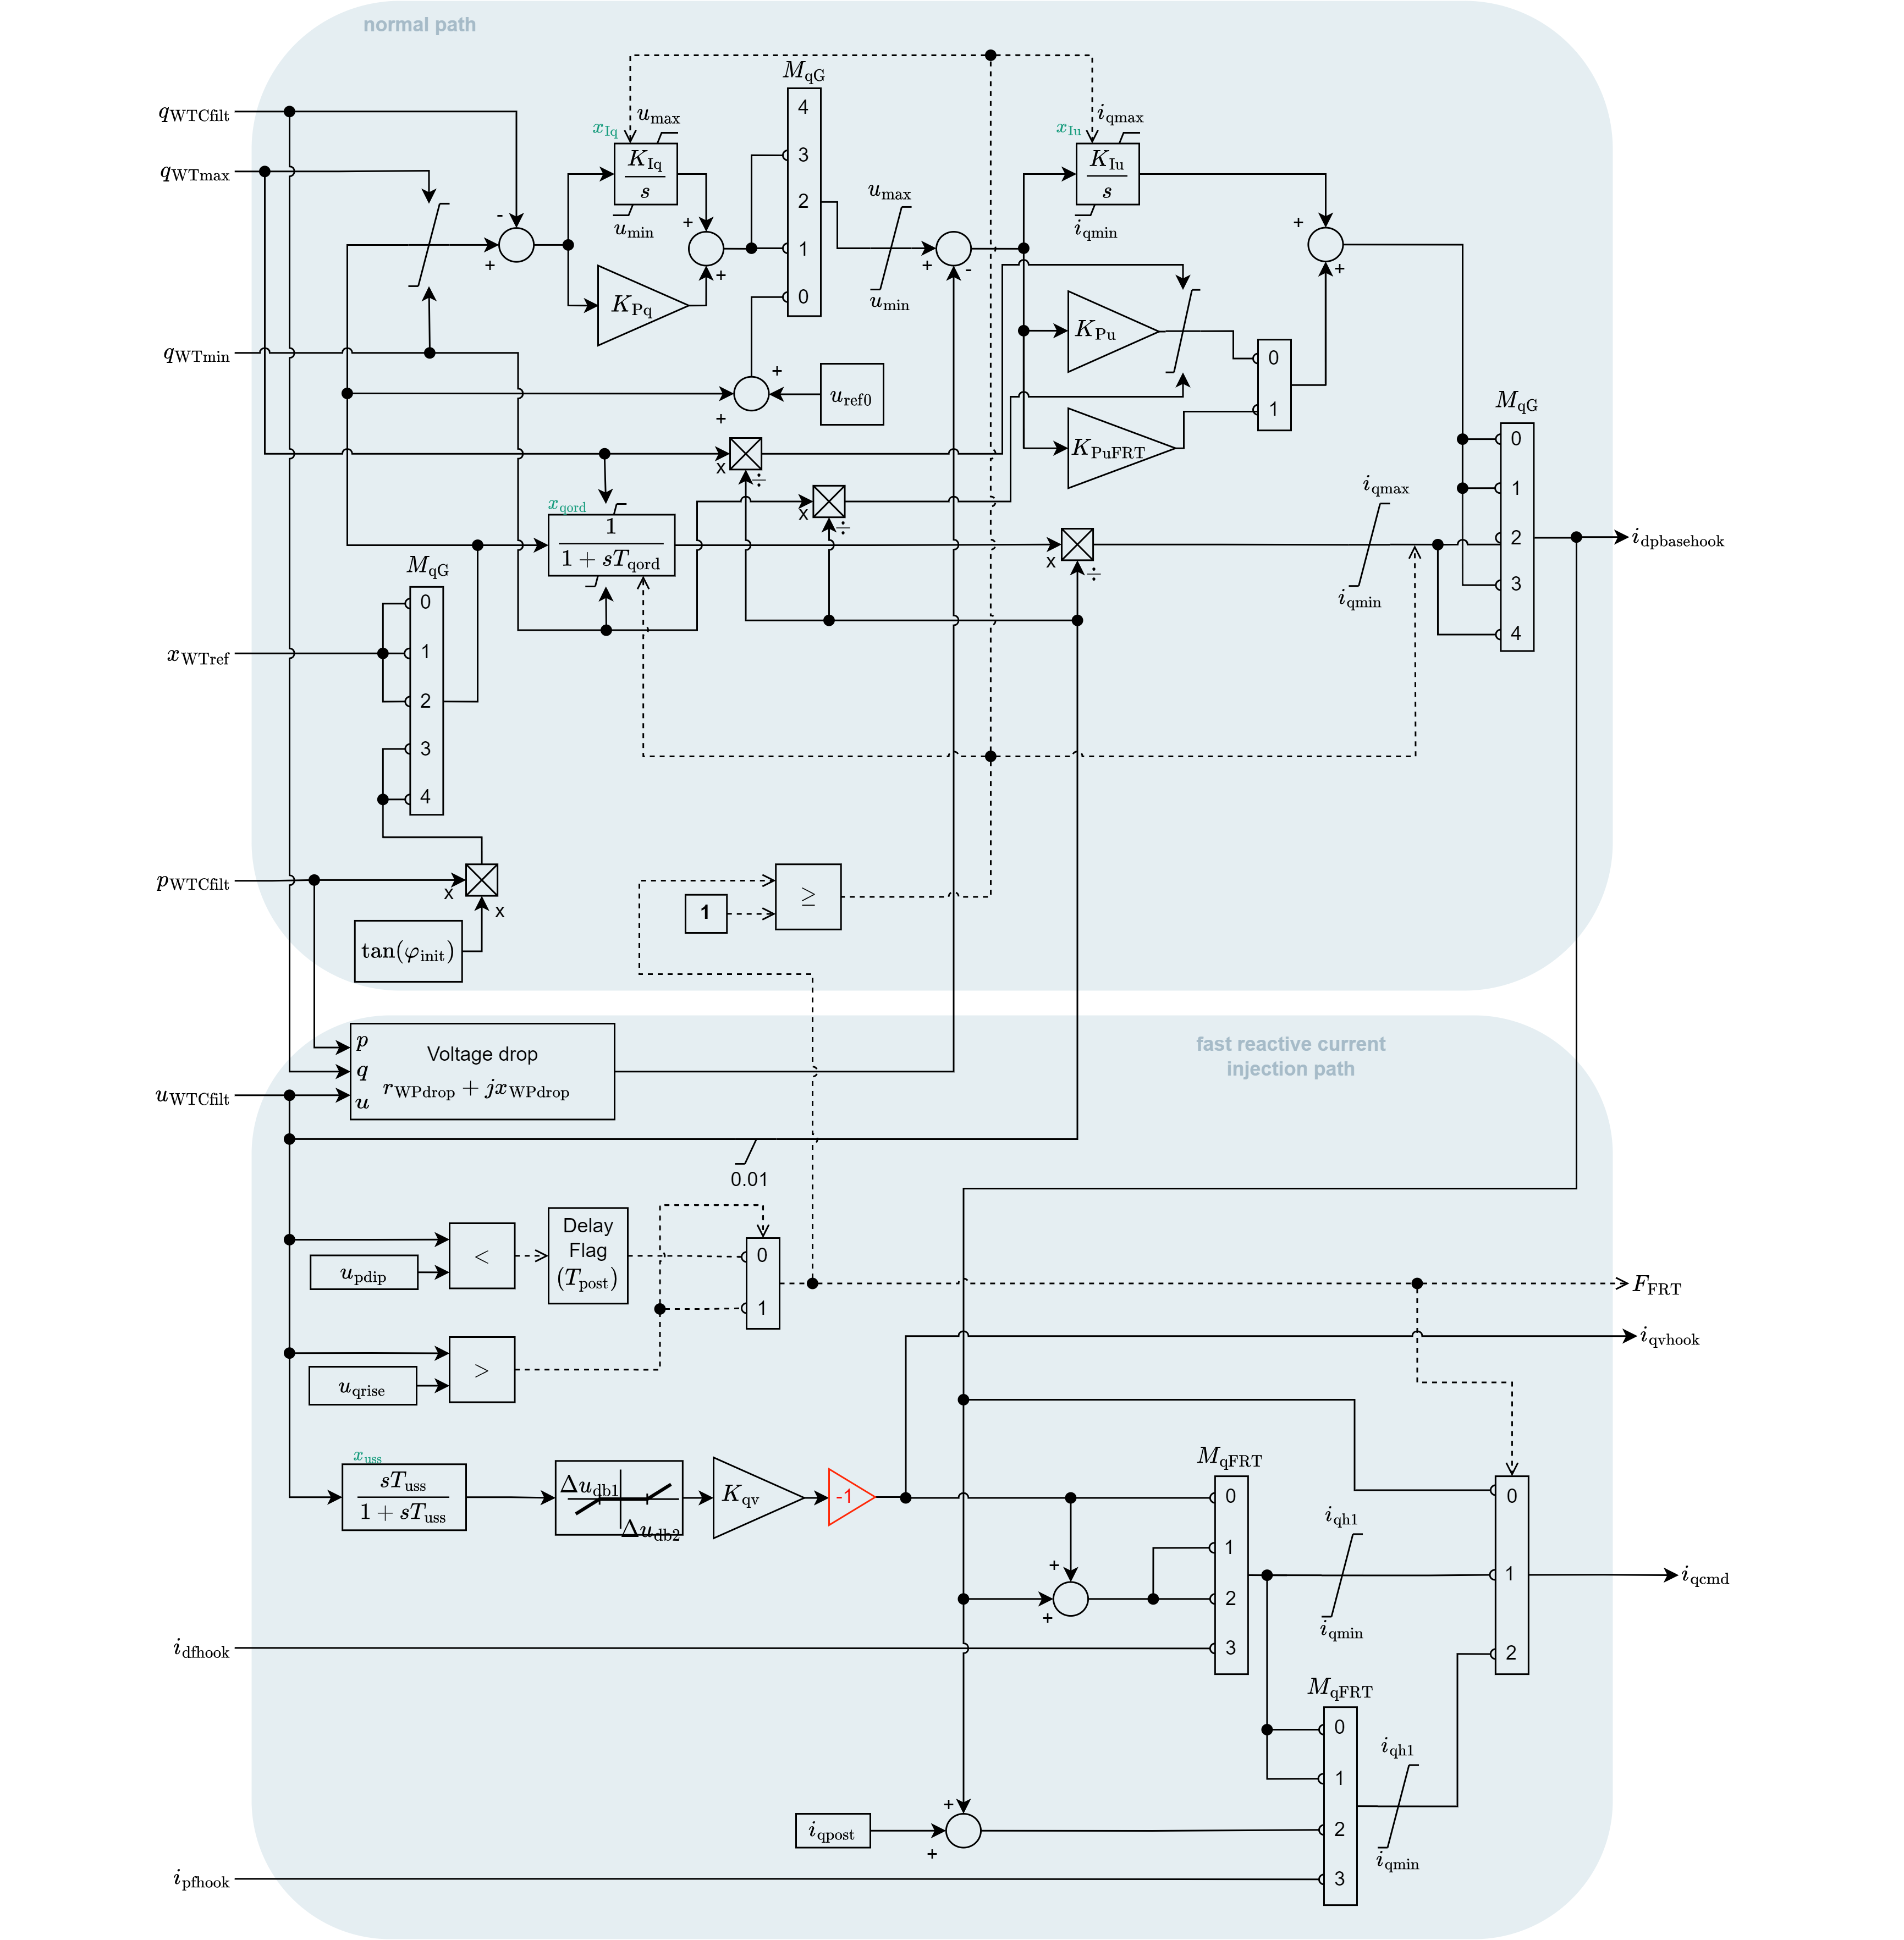
\includegraphics{drawings/WT_Q_control.drawio.png}

}

\caption{\label{fig-QControlModule}Wind turbine Q control module, based
on {[}1{]}}

\end{figure}%

The WT Q Control Module consists of a normal path and a fast reactive
current injection path, which acts during and some time after an event
(voltage drop or rise). There are multiple possible operating modes for
each path, described in detail in {[}7{]}.

Depending on the mode, \(x_\mathrm{WTref}\) can be a voltage or reactive
power setpoint.

The available control modes are listed in
Table~\ref{tbl-qControlModesNormal} and
Table~\ref{tbl-qControlModesFast}. The following descriptions have been
based on {[}7{]} and {[}1{]}.

For example in mode 1, the normal path consists of two cascaded
Proportional-Integral (PI) controllers. The first one (reactive power
controller) controls reactive power by generating a voltage reference
for the second controller (voltage controller), which then generates the
reactive current command \(i_\mathrm{qbasehook}\). Input and output
limitations are applied.

During faults, the fast injection path adds an additional component to
the q-axis current which is computed based on the voltage deviation
\(\Delta u\), a dead-band and droop (gain \(K_\mathrm{qv}\)).

Special attention must be paid to the reactive current signs in {[}1{]},
as they seem to be inconsistent {[}7{]}. In the fast injection path,
\(u_\mathrm{WTC}\) voltage drop leads to \(\Delta u < 0\), resulting in
\(i_\mathrm{qvhook} < 0\). This behavior is opposite to the normal path.
To solve this, the fast injection path's sign can be inverted, as has
been done in Figure~\ref{fig-QControlModule} (red -1 block).

\begin{longtable}[]{@{}
  >{\raggedright\arraybackslash}p{(\columnwidth - 2\tabcolsep) * \real{0.1648}}
  >{\raggedright\arraybackslash}p{(\columnwidth - 2\tabcolsep) * \real{0.8352}}@{}}
\caption{Q control normal path control modes, based on
{[}1{]}}\label{tbl-qControlModesNormal}\tabularnewline
\toprule\noalign{}
\begin{minipage}[b]{\linewidth}\raggedright
\(M_\mathrm{qG}\)
\end{minipage} & \begin{minipage}[b]{\linewidth}\raggedright
Description
\end{minipage} \\
\midrule\noalign{}
\endfirsthead
\toprule\noalign{}
\begin{minipage}[b]{\linewidth}\raggedright
\(M_\mathrm{qG}\)
\end{minipage} & \begin{minipage}[b]{\linewidth}\raggedright
Description
\end{minipage} \\
\midrule\noalign{}
\endhead
\bottomrule\noalign{}
\endlastfoot
0 & Voltage control \\
1 & Reactive power control \\
2 & Open loop reactive power control (only used with closed loop at
plant level) \\
3 & Power factor control \\
4 & Open loop power factor control \\
\end{longtable}

\begin{longtable}[]{@{}
  >{\raggedright\arraybackslash}p{(\columnwidth - 4\tabcolsep) * \real{0.1172}}
  >{\raggedright\arraybackslash}p{(\columnwidth - 4\tabcolsep) * \real{0.6552}}
  >{\raggedright\arraybackslash}p{(\columnwidth - 4\tabcolsep) * \real{0.2276}}@{}}
\caption{Q control reactive current injection path control modes, based
on {[}1{]}}\label{tbl-qControlModesFast}\tabularnewline
\toprule\noalign{}
\begin{minipage}[b]{\linewidth}\raggedright
\(M_\mathrm{qFRT}\)
\end{minipage} & \begin{minipage}[b]{\linewidth}\raggedright
During Fault
\end{minipage} & \begin{minipage}[b]{\linewidth}\raggedright
Post Fault
\end{minipage} \\
\midrule\noalign{}
\endfirsthead
\toprule\noalign{}
\begin{minipage}[b]{\linewidth}\raggedright
\(M_\mathrm{qFRT}\)
\end{minipage} & \begin{minipage}[b]{\linewidth}\raggedright
During Fault
\end{minipage} & \begin{minipage}[b]{\linewidth}\raggedright
Post Fault
\end{minipage} \\
\midrule\noalign{}
\endhead
\bottomrule\noalign{}
\endlastfoot
0 & A function of the voltage change compared to the pre-fault voltage &
Same function as during fault \\
1 & Pre-fault current plus a term depending on the voltage change
compared to the pre-fault voltage & Same function as during fault \\
2 & Pre-fault current plus a term depending on the voltage change
compared to the pre-fault voltage & Pre-fault current plus a constant \\
3 & User defined & User defined \\
\end{longtable}

\subsubsection{Parameters}\label{parameters}

\begin{longtable}[]{@{}
  >{\raggedright\arraybackslash}p{(\columnwidth - 10\tabcolsep) * \real{0.0600}}
  >{\raggedright\arraybackslash}p{(\columnwidth - 10\tabcolsep) * \real{0.0600}}
  >{\raggedright\arraybackslash}p{(\columnwidth - 10\tabcolsep) * \real{0.0500}}
  >{\raggedright\arraybackslash}p{(\columnwidth - 10\tabcolsep) * \real{0.2000}}
  >{\raggedright\arraybackslash}p{(\columnwidth - 10\tabcolsep) * \real{0.4400}}
  >{\raggedright\arraybackslash}p{(\columnwidth - 10\tabcolsep) * \real{0.0700}}@{}}
\caption{Parameters of WT Q control, based on {[}1{]} and
\emph{DIgSILENT
PowerFactory}}\label{tbl-parametersQControl}\tabularnewline
\toprule\noalign{}
\begin{minipage}[b]{\linewidth}\raggedright
name
\end{minipage} & \begin{minipage}[b]{\linewidth}\raggedright
type
\end{minipage} & \begin{minipage}[b]{\linewidth}\raggedright
unit
\end{minipage} & \begin{minipage}[b]{\linewidth}\raggedright
base
\end{minipage} & \begin{minipage}[b]{\linewidth}\raggedright
description
\end{minipage} & \begin{minipage}[b]{\linewidth}\raggedright
typical value
\end{minipage} \\
\midrule\noalign{}
\endfirsthead
\toprule\noalign{}
\begin{minipage}[b]{\linewidth}\raggedright
name
\end{minipage} & \begin{minipage}[b]{\linewidth}\raggedright
type
\end{minipage} & \begin{minipage}[b]{\linewidth}\raggedright
unit
\end{minipage} & \begin{minipage}[b]{\linewidth}\raggedright
base
\end{minipage} & \begin{minipage}[b]{\linewidth}\raggedright
description
\end{minipage} & \begin{minipage}[b]{\linewidth}\raggedright
typical value
\end{minipage} \\
\midrule\noalign{}
\endhead
\bottomrule\noalign{}
\endlastfoot
\(\Delta u_\mathrm{db1}\) & float & pu & \(U_\mathrm{base}\) & Voltage
difference dead band lower limit & -0.1 \\
\(\Delta u_\mathrm{db2}\) & float & pu & \(U_\mathrm{base}\) & Voltage
differnce dead band upper limit & 0.1 \\
\(i_\mathrm{qh1}\) & float & pu & \(I_\mathrm{base}\) & Maximum reactive
current injection during FRT & 1.05 \\
\(i_\mathrm{qmax}\) & float & pu & \(I_\mathrm{base}\) & Maximum
reactive current injection & 1.05 \\
\(i_\mathrm{qmin}\) & float & pu & \(I_\mathrm{base}\) & Minimum
reactive current injection & -1.05 \\
\(i_\mathrm{qpost}\) & float & pu & \(I_\mathrm{base}\) & Post-fault
reactive current injection & 0 \\
\(K_\mathrm{Iq}\) & float & pu & \(U_\mathrm{base}/S_\mathrm{base}/s\) &
Q PI controller integral gain & 2 \\
\(K_\mathrm{Iu}\) & float & pu & \(I_\mathrm{base}/U_\mathrm{base}/s\) &
U PI controller integral gain & 2 \\
\(K_\mathrm{Pq}\) & float & pu & \(U_\mathrm{base}/S_\mathrm{base}\) & Q
PI controller proportional gain & 0 \\
\(K_\mathrm{Pu}\) & float & pu & \(I_\mathrm{base}/U_\mathrm{base}\) & U
PI controller proportional gain & 2 \\
\(K_\mathrm{PuFRT}\) & float & pu & \(I_\mathrm{base}/U_\mathrm{base}\)
& U PI controller proportional gain during FRT & 0 \\
\(K_\mathrm{qv}\) & float & pu & \(I_\mathrm{base}/U_\mathrm{base}\) &
Droop for fast reactive current injection & 2 \\
\(M_\mathrm{qFRT}\) & bool & - & - & Fast reactive current injection Q
control mode (Table~\ref{tbl-qControlModesFast}) & 2 \\
\(M_\mathrm{qG}\) & bool & - & - & Normal path Q control mode
(Table~\ref{tbl-qControlModesNormal}) & 1 \\
\(r_\mathrm{drop}\) & float & pu & \(Z_\mathrm{base}\) & Voltage drop
resistance & 0 \\
\(T_\mathrm{post}\) & float & s & - & Duration of post-fault period &
0 \\
\(T_\mathrm{qord}\) & float & s & - & Time constant in reactive power
order lag & 0 \\
\(T_\mathrm{uss}\) & float & s & - & Steady state voltage filter time
constant & 30 \\
\(u_\mathrm{max}\) & float & pu & \(U_\mathrm{base}\) & Upper limit in U
PI controller integrator & 2 \\
\(u_\mathrm{min}\) & float & pu & \(U_\mathrm{base}\) & Lower limit in U
PI controller integrator & 0 \\
\(u_\mathrm{qdip}\) & float & pu & \(U_\mathrm{base}\) & Q control:
voltage threshold for UVRT detection & 0.9 \\
\(u_\mathrm{qrise}\) & float & pu & \(U_\mathrm{base}\) & Q Control:
Voltage threshold for OVRT detection & 1.1 \\
\(u_\mathrm{ref0}\) & float & pu & \(U_\mathrm{base}\) & Voltage
reference bias & 0 \\
\(x_\mathrm{drop}\) & float & pu & \(Z_\mathrm{base}\) & Voltage drop
reactance & 0 \\
\end{longtable}

\subsubsection{Variables:}\label{variables-1}

\paragraph{Inputs}\label{inputs-1}

\begin{longtable}[]{@{}
  >{\raggedright\arraybackslash}p{(\columnwidth - 8\tabcolsep) * \real{0.1439}}
  >{\raggedright\arraybackslash}p{(\columnwidth - 8\tabcolsep) * \real{0.0360}}
  >{\raggedright\arraybackslash}p{(\columnwidth - 8\tabcolsep) * \real{0.0288}}
  >{\raggedright\arraybackslash}p{(\columnwidth - 8\tabcolsep) * \real{0.1223}}
  >{\raggedright\arraybackslash}p{(\columnwidth - 8\tabcolsep) * \real{0.6691}}@{}}
\caption{Inputs, based on {[}1{]} and
{[}5{]}}\label{tbl-inputsQControl}\tabularnewline
\toprule\noalign{}
\begin{minipage}[b]{\linewidth}\raggedright
name
\end{minipage} & \begin{minipage}[b]{\linewidth}\raggedright
type
\end{minipage} & \begin{minipage}[b]{\linewidth}\raggedright
unit
\end{minipage} & \begin{minipage}[b]{\linewidth}\raggedright
base
\end{minipage} & \begin{minipage}[b]{\linewidth}\raggedright
description
\end{minipage} \\
\midrule\noalign{}
\endfirsthead
\toprule\noalign{}
\begin{minipage}[b]{\linewidth}\raggedright
name
\end{minipage} & \begin{minipage}[b]{\linewidth}\raggedright
type
\end{minipage} & \begin{minipage}[b]{\linewidth}\raggedright
unit
\end{minipage} & \begin{minipage}[b]{\linewidth}\raggedright
base
\end{minipage} & \begin{minipage}[b]{\linewidth}\raggedright
description
\end{minipage} \\
\midrule\noalign{}
\endhead
\bottomrule\noalign{}
\endlastfoot
\(i_\mathrm{dfhook}\) & float & pu & \(I_\mathrm{base}\) & user-defined
input for during-fault reactive current \\
\(i_\mathrm{pfhook}\) & float & pu & \(I_\mathrm{base}\) & user-defined
input for post-fault period reactive current \\
\(p_\mathrm{WTCfilt}\) & float & pu & \(S_\mathrm{base}\) & measured
active power \\
\(q_\mathrm{WTCfilt}\) & float & pu & \(S_\mathrm{base}\) & measured
reactive power \\
\(q_\mathrm{WTmax}\) & float & pu & \(S_\mathrm{base}\) & maximum
reactive power from Q limitation module (may be used to implement a
capability curve) \\
\(q_\mathrm{WTmin}\) & float & pu & \(S_\mathrm{base}\) & minimum
reactive power from Q limitation module (may be used to implement a
capability curve) \\
\(u_\mathrm{WTCfilt}\) & float & pu & \(U_\mathrm{base}\) & measured
voltage \\
\(x_\mathrm{WTref}\) & float & pu & \(Z_\mathrm{base}\) & voltage or
reactive power reference, depending on control mode \\
\end{longtable}

\paragraph{Outputs}\label{outputs-1}

\begin{longtable}[]{@{}
  >{\raggedright\arraybackslash}p{(\columnwidth - 8\tabcolsep) * \real{0.1774}}
  >{\raggedright\arraybackslash}p{(\columnwidth - 8\tabcolsep) * \real{0.0565}}
  >{\raggedright\arraybackslash}p{(\columnwidth - 8\tabcolsep) * \real{0.0323}}
  >{\raggedright\arraybackslash}p{(\columnwidth - 8\tabcolsep) * \real{0.1371}}
  >{\raggedright\arraybackslash}p{(\columnwidth - 8\tabcolsep) * \real{0.5968}}@{}}
\caption{Outputs, based on
{[}1{]}}\label{tbl-outputsQControl}\tabularnewline
\toprule\noalign{}
\begin{minipage}[b]{\linewidth}\raggedright
name
\end{minipage} & \begin{minipage}[b]{\linewidth}\raggedright
type
\end{minipage} & \begin{minipage}[b]{\linewidth}\raggedright
unit
\end{minipage} & \begin{minipage}[b]{\linewidth}\raggedright
base
\end{minipage} & \begin{minipage}[b]{\linewidth}\raggedright
description
\end{minipage} \\
\midrule\noalign{}
\endfirsthead
\toprule\noalign{}
\begin{minipage}[b]{\linewidth}\raggedright
name
\end{minipage} & \begin{minipage}[b]{\linewidth}\raggedright
type
\end{minipage} & \begin{minipage}[b]{\linewidth}\raggedright
unit
\end{minipage} & \begin{minipage}[b]{\linewidth}\raggedright
base
\end{minipage} & \begin{minipage}[b]{\linewidth}\raggedright
description
\end{minipage} \\
\midrule\noalign{}
\endhead
\bottomrule\noalign{}
\endlastfoot
\(F_\mathrm{FRT}\) & integer & - & - & Fault signal: 0=no fault,
1=fault, 2=post-fault \\
\(i_\mathrm{qbasehook}\) & float & pu & \(I_\mathrm{base}\) & Normal
path component of reactive current command \\
\(I_\mathrm{qcmd}\) & float & - & \(I_\mathrm{base}\) & reactive current
command \\
\(I_\mathrm{qvhook}\) & float & - & \(I_\mathrm{base}\) & Fast reactive
current injection path component of reactive current command \\
\end{longtable}

\subsubsection{Initial equations}\label{initial-equations-1}

For the used initialization helper variables, see
Section~\ref{sec-initHelpersGlobal}.

\begin{equation}\phantomsection\label{eq-initXiu}{
x_\mathrm{Iu\,0} = x_\mathrm{qord\,0} = Q_\mathrm{ord\,0}/U_\mathrm{0}
}\end{equation}

\begin{equation}\phantomsection\label{eq-initXiq}{
x_\mathrm{Iq\,0} = U_\mathrm{0}
}\end{equation}

\begin{equation}\phantomsection\label{eq-initXuss}{
x_\mathrm{uss\,0} = 0
}\end{equation}

\subsection{Q limitation}\label{q-limitation}

\begin{figure}

\centering{

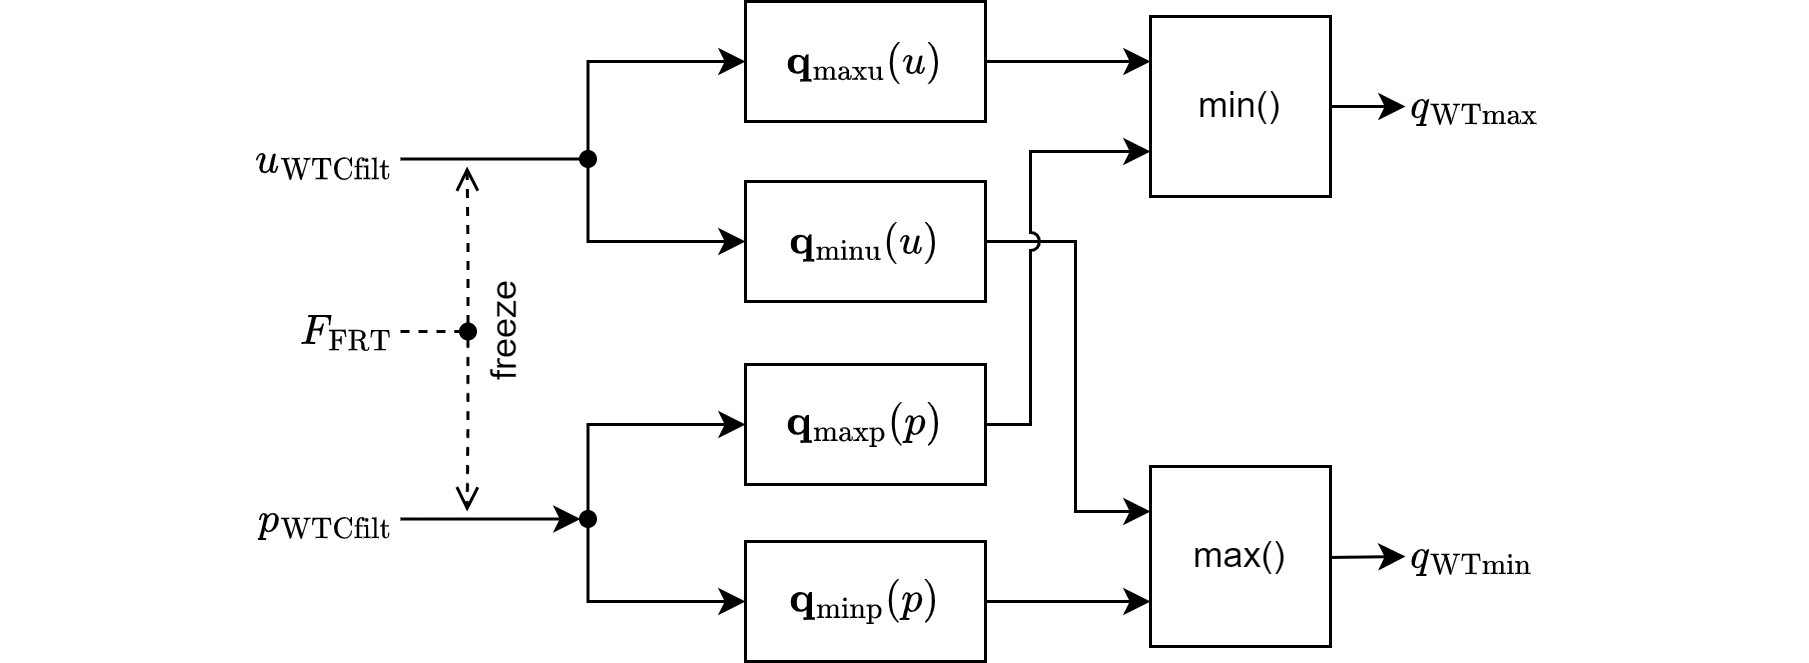
\includegraphics{drawings/WT_Qlim.drawio.png}

}

\caption{\label{fig-WTQLim}WT Q limitation module, based on {[}1{]}}

\end{figure}%

The Q limitation module consists of a set of lookup-tables that
determine the maximum and minimum reactive power that can be supplied by
the WT depending on active power and voltage. It can be used to
implement the generator's capability curve.

\subsubsection{Parameters}\label{parameters-1}

\begin{longtable}[]{@{}
  >{\raggedright\arraybackslash}p{(\columnwidth - 10\tabcolsep) * \real{0.1000}}
  >{\raggedright\arraybackslash}p{(\columnwidth - 10\tabcolsep) * \real{0.0600}}
  >{\raggedright\arraybackslash}p{(\columnwidth - 10\tabcolsep) * \real{0.0500}}
  >{\raggedright\arraybackslash}p{(\columnwidth - 10\tabcolsep) * \real{0.2000}}
  >{\raggedright\arraybackslash}p{(\columnwidth - 10\tabcolsep) * \real{0.4400}}
  >{\raggedright\arraybackslash}p{(\columnwidth - 10\tabcolsep) * \real{0.1500}}@{}}
\caption{Parameters of mechanical moduele, based on {[}1{]} and
\emph{DIgSILENT
PowerFactory}}\label{tbl-parametersWTQlim}\tabularnewline
\toprule\noalign{}
\begin{minipage}[b]{\linewidth}\raggedright
name
\end{minipage} & \begin{minipage}[b]{\linewidth}\raggedright
type
\end{minipage} & \begin{minipage}[b]{\linewidth}\raggedright
unit
\end{minipage} & \begin{minipage}[b]{\linewidth}\raggedright
base
\end{minipage} & \begin{minipage}[b]{\linewidth}\raggedright
description
\end{minipage} & \begin{minipage}[b]{\linewidth}\raggedright
typical value
\end{minipage} \\
\midrule\noalign{}
\endfirsthead
\toprule\noalign{}
\begin{minipage}[b]{\linewidth}\raggedright
name
\end{minipage} & \begin{minipage}[b]{\linewidth}\raggedright
type
\end{minipage} & \begin{minipage}[b]{\linewidth}\raggedright
unit
\end{minipage} & \begin{minipage}[b]{\linewidth}\raggedright
base
\end{minipage} & \begin{minipage}[b]{\linewidth}\raggedright
description
\end{minipage} & \begin{minipage}[b]{\linewidth}\raggedright
typical value
\end{minipage} \\
\midrule\noalign{}
\endhead
\bottomrule\noalign{}
\endlastfoot
\(\mathbf{q_\mathrm{maxp}}(p)\) & lookup-table & pu &
\(S_\mathrm{base}\) & Maximum Q as a function of P & {[}0,0; 0.3,0.33;
1,0.33{]} \\
\(\mathbf{q_\mathrm{maxu}}(u)\) & lookup-table & pu &
\(S_\mathrm{base}\) & Maximum Q as a function of U & {[}0,0; 0.8,0.33;
0.9,0.33{]} \\
\(\mathbf{q_\mathrm{minp}}(p)\) & lookup-table & pu &
\(S_\mathrm{base}\) & Minimum Q as a function of P & {[}0,0; 0.3,-0.33;
1,-0.33{]} \\
\(\mathbf{q_\mathrm{minu}}(u)\) & lookup-table & pu &
\(S_\mathrm{base}\) & Minimum Q as a function of U & {[}0,0; 0.8,-0.33;
0.9,-0.33{]} \\
\end{longtable}

\subsubsection{Variables}\label{variables-2}

\paragraph{Inputs}\label{inputs-2}

\begin{longtable}[]{@{}
  >{\raggedright\arraybackslash}p{(\columnwidth - 8\tabcolsep) * \real{0.2128}}
  >{\raggedright\arraybackslash}p{(\columnwidth - 8\tabcolsep) * \real{0.0745}}
  >{\raggedright\arraybackslash}p{(\columnwidth - 8\tabcolsep) * \real{0.0426}}
  >{\raggedright\arraybackslash}p{(\columnwidth - 8\tabcolsep) * \real{0.1809}}
  >{\raggedright\arraybackslash}p{(\columnwidth - 8\tabcolsep) * \real{0.4894}}@{}}
\caption{Inputs, based on
{[}1{]}}\label{tbl-inputsWTQlim}\tabularnewline
\toprule\noalign{}
\begin{minipage}[b]{\linewidth}\raggedright
name
\end{minipage} & \begin{minipage}[b]{\linewidth}\raggedright
type
\end{minipage} & \begin{minipage}[b]{\linewidth}\raggedright
unit
\end{minipage} & \begin{minipage}[b]{\linewidth}\raggedright
base
\end{minipage} & \begin{minipage}[b]{\linewidth}\raggedright
description
\end{minipage} \\
\midrule\noalign{}
\endfirsthead
\toprule\noalign{}
\begin{minipage}[b]{\linewidth}\raggedright
name
\end{minipage} & \begin{minipage}[b]{\linewidth}\raggedright
type
\end{minipage} & \begin{minipage}[b]{\linewidth}\raggedright
unit
\end{minipage} & \begin{minipage}[b]{\linewidth}\raggedright
base
\end{minipage} & \begin{minipage}[b]{\linewidth}\raggedright
description
\end{minipage} \\
\midrule\noalign{}
\endhead
\bottomrule\noalign{}
\endlastfoot
\(F_\mathrm{FRT}\) & boolean & - & - & WT Fault Ride Through (FRT) flag
signal \\
\(p_\mathrm{WTCfilt}\) & float & pu & \(S_\mathrm{base}\) & Measured
active power at the WT terminal \\
\(u_\mathrm{WTCfilt}\) & float & pu & \(U_\mathrm{base}\) & Measured
voltage of the WT terminal \\
\end{longtable}

\paragraph{Outputs}\label{outputs-2}

\begin{longtable}[]{@{}
  >{\raggedright\arraybackslash}p{(\columnwidth - 8\tabcolsep) * \real{0.2817}}
  >{\raggedright\arraybackslash}p{(\columnwidth - 8\tabcolsep) * \real{0.0704}}
  >{\raggedright\arraybackslash}p{(\columnwidth - 8\tabcolsep) * \real{0.0563}}
  >{\raggedright\arraybackslash}p{(\columnwidth - 8\tabcolsep) * \real{0.2394}}
  >{\raggedright\arraybackslash}p{(\columnwidth - 8\tabcolsep) * \real{0.3521}}@{}}
\caption{Outputs, based on
{[}1{]}}\label{tbl-outputsWTQlim}\tabularnewline
\toprule\noalign{}
\begin{minipage}[b]{\linewidth}\raggedright
name
\end{minipage} & \begin{minipage}[b]{\linewidth}\raggedright
type
\end{minipage} & \begin{minipage}[b]{\linewidth}\raggedright
unit
\end{minipage} & \begin{minipage}[b]{\linewidth}\raggedright
base
\end{minipage} & \begin{minipage}[b]{\linewidth}\raggedright
description
\end{minipage} \\
\midrule\noalign{}
\endfirsthead
\toprule\noalign{}
\begin{minipage}[b]{\linewidth}\raggedright
name
\end{minipage} & \begin{minipage}[b]{\linewidth}\raggedright
type
\end{minipage} & \begin{minipage}[b]{\linewidth}\raggedright
unit
\end{minipage} & \begin{minipage}[b]{\linewidth}\raggedright
base
\end{minipage} & \begin{minipage}[b]{\linewidth}\raggedright
description
\end{minipage} \\
\midrule\noalign{}
\endhead
\bottomrule\noalign{}
\endlastfoot
\(q_\mathrm{WTmax}\) & float & pu & \(S_\mathrm{base}\) & Maximum WT
reactive power \\
\(q_\mathrm{WTmin}\) & float & pu & \(S_\mathrm{base}\) & Minimum WT
reactive power \\
\end{longtable}

\subsection{Current limitation}\label{current-limitation}

The current limitation acts after the P and Q controls as shown in
Figure~\ref{fig-wtControlSubstructure}. The priority between active and
reactive current can be set by \(M_\mathrm{qpri}\). Outside FRT,
P-Priority is always active regardless of \(M_\mathrm{qpri}\).

Current is limited to the maximum admissible current \(i_\mathrm{max}\).
During FRT there is a separate maximum current value
\(i_\mathrm{maxdip}\).

In addition to \(i_\mathrm{max}\), Voltage Dependent Limits (VDL) are
defined for active and reactive current components through the look-up
tables \(\mathbf{i_\mathrm{pmax}}(u_\mathrm{WT})\) and
\(\mathbf{i_\mathrm{qmax}}(u_\mathrm{WT})\).

The current limitation contains an additional high-voltage current limit
logic (Kpqu-logic), which limits voltage-supporting reactive current
injection when voltage is already high (parameters
\(u_\mathrm{pqumax}\), \(K_\mathrm{pqu}\)).

The following Figure~\ref{fig-currentLimCode} shows a python inspired
pseudo-code implementation of the the current limitation as shown in
{[}7{]}.

\begin{figure}

\centering{

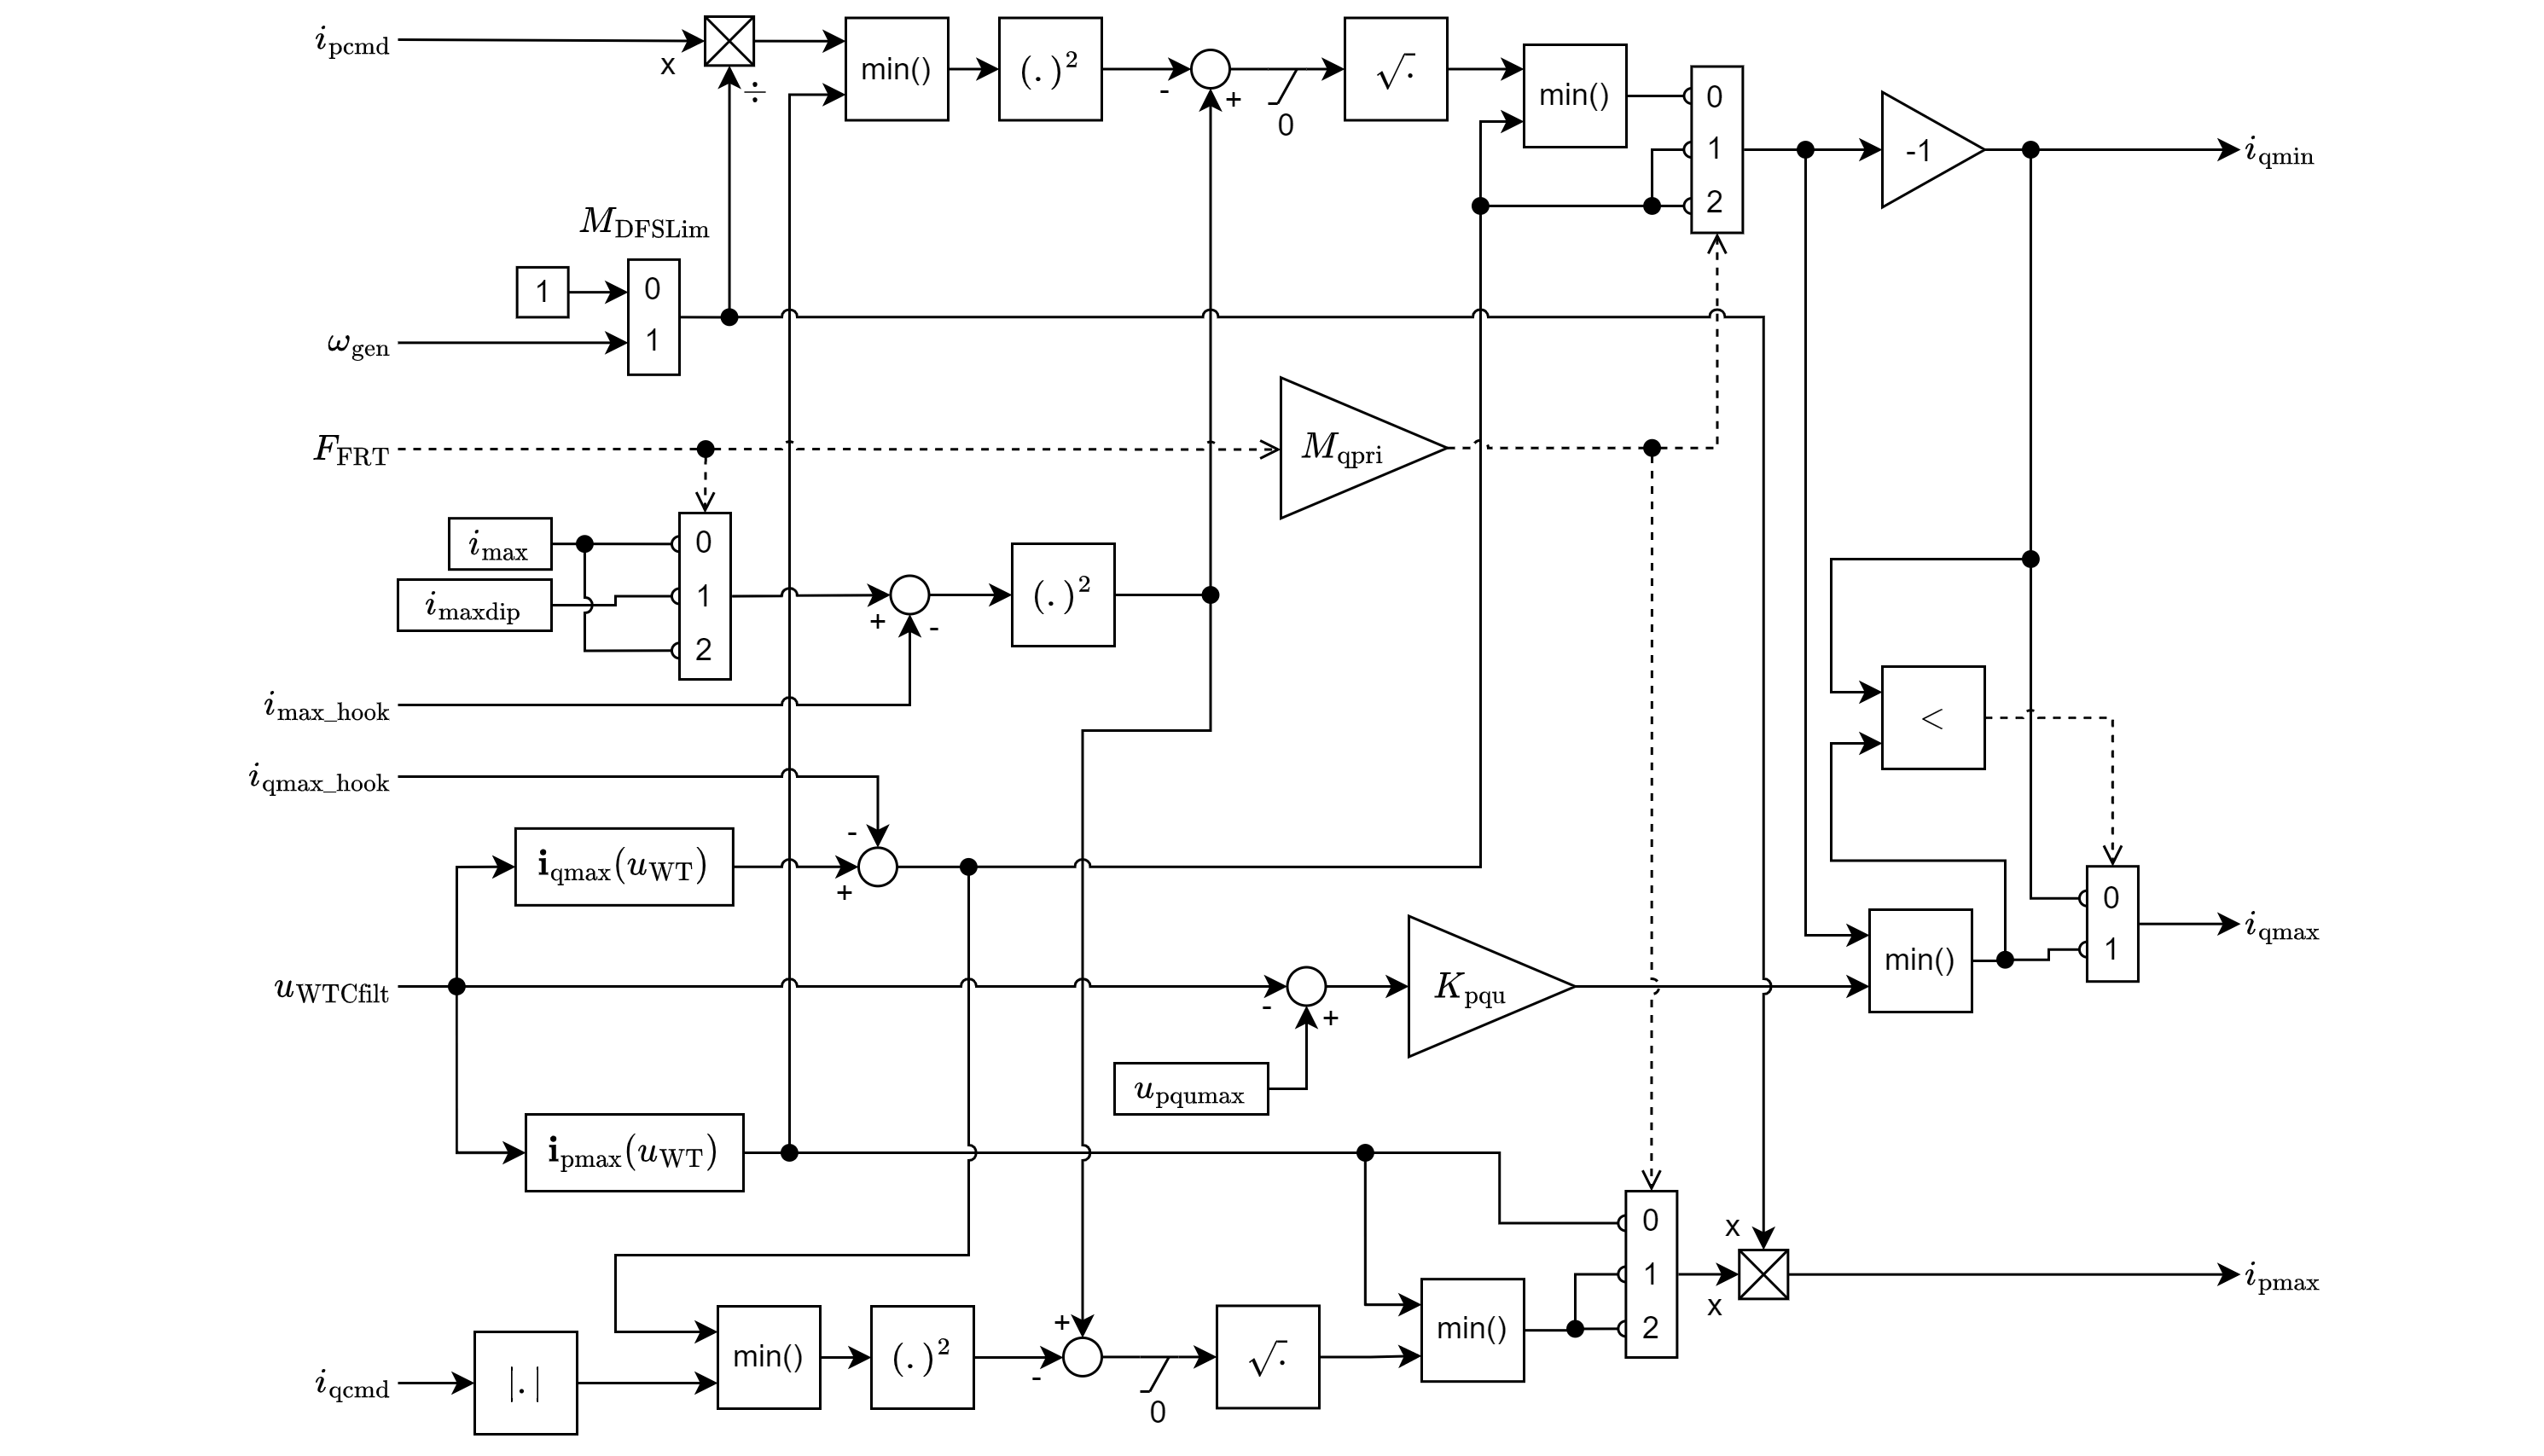
\includegraphics{drawings/WT_CurrentLim.drawio.png}

}

\caption{\label{fig-WTCurrentLim}Wind turbine current limitation, based
on {[}1{]}}

\end{figure}%

\begin{figure}

\centering{

\begin{verbatim}
M_DFSLim,imax_hook,iqmax_hook = (0,0,0)
if F_FRT == 1:
    i_maxset = i_maxdip
else: 
    i_maxset = i_max
# P Priority
if (M_qpri == 0) or (F_FRT == 0):
    i_pmax = i_pmaxVDL(u_WTCfilt)
    
    i_qlimit = min(
        i_qmaxVDL(u_WTCfilt),
        sqrt(max(0,
            i_maxset**2 - min(
                i_pcmd, 
                i_pmaxVDL(u_WTCfilt))**2) 
    ))
    i_qmin = -i_qlimit
    i_qmax = K_pqulogic(i_qlimit)
# Q Priority
else: 
    i_qlimit = i_qmaxVDL(u_WTCfilt)
    
    i_qmin = -i_qlimit
    i_qmax = K_pqulogic(i_qlimit)
    i_pmax = min(
        i_pmaxVDL(u_WTCfilt),
        sqrt(max(0,
            i_maxset**2 - min(
                abs(i_qcmd), 
                i_qmaxVDL(u_WTCfilt))**2)
    ))
\end{verbatim}

}

\caption{\label{fig-currentLimCode}Python-inspired pseoudo code
implementation of the current limitation block {[}7{]}}

\end{figure}%

\subsubsection{Parameters}\label{parameters-2}

\begin{longtable}[]{@{}
  >{\raggedright\arraybackslash}p{(\columnwidth - 10\tabcolsep) * \real{0.1000}}
  >{\raggedright\arraybackslash}p{(\columnwidth - 10\tabcolsep) * \real{0.0700}}
  >{\raggedright\arraybackslash}p{(\columnwidth - 10\tabcolsep) * \real{0.0500}}
  >{\raggedright\arraybackslash}p{(\columnwidth - 10\tabcolsep) * \real{0.2000}}
  >{\raggedright\arraybackslash}p{(\columnwidth - 10\tabcolsep) * \real{0.4400}}
  >{\raggedright\arraybackslash}p{(\columnwidth - 10\tabcolsep) * \real{0.1500}}@{}}
\caption{Parameters of mechanical moduele, based on {[}1{]} and
\emph{DIgSILENT
PowerFactory}}\label{tbl-parametersCurrentLim}\tabularnewline
\toprule\noalign{}
\begin{minipage}[b]{\linewidth}\raggedright
name
\end{minipage} & \begin{minipage}[b]{\linewidth}\raggedright
type
\end{minipage} & \begin{minipage}[b]{\linewidth}\raggedright
unit
\end{minipage} & \begin{minipage}[b]{\linewidth}\raggedright
base
\end{minipage} & \begin{minipage}[b]{\linewidth}\raggedright
description
\end{minipage} & \begin{minipage}[b]{\linewidth}\raggedright
typical value
\end{minipage} \\
\midrule\noalign{}
\endfirsthead
\toprule\noalign{}
\begin{minipage}[b]{\linewidth}\raggedright
name
\end{minipage} & \begin{minipage}[b]{\linewidth}\raggedright
type
\end{minipage} & \begin{minipage}[b]{\linewidth}\raggedright
unit
\end{minipage} & \begin{minipage}[b]{\linewidth}\raggedright
base
\end{minipage} & \begin{minipage}[b]{\linewidth}\raggedright
description
\end{minipage} & \begin{minipage}[b]{\linewidth}\raggedright
typical value
\end{minipage} \\
\midrule\noalign{}
\endhead
\bottomrule\noalign{}
\endlastfoot
\(i_\mathrm{max}\) & float & pu & \(I_\mathrm{base}\) & WT terminal
maximum admissible current & 1.3 \\
\(i_\mathrm{maxdip}\) & float & pu & \(I_\mathrm{base}\) & WT terminal
maximum admissible current during fault & 1.3 \\
\(\mathbf{i_\mathrm{pmax}}(u_\mathrm{WT})\) & lookup-table & pu &
\(I_\mathrm{base}\) & lookup-table for maximum active current as a
function of voltage & {[}0,0; 0.1,0; 0.15,1; 0.9,1; 0.91,1.2;
1.2,1.2{]} \\
\(\mathbf{i_\mathrm{qmax}}(u_\mathrm{WT})\) & lookup-table & pu &
\(I_\mathrm{base}\) & lookup-table for maximum reactive current as a
function of voltage & {[}0,0.1; 0.2,0.95; 0.2,1; 0.9,1; 0.9,0.36;
1.1,0.3{]} \\
\(K_\mathrm{pqu}\) & float & pu & \(I_\mathrm{base}/U_\mathrm{base}\) &
Droop of reactive current limit with resepect to voltage & 20 \\
\(M_\mathrm{DFSLim}\) & boolean & - & - & Type 3 stator current
limitation (false = total current limitation, true = stator current
limitation) & false \\
\(M_\mathrm{qpri}\) & boolean & - & - & Active or reactive power
priority during fault (false = active power priority, true = reactive
power priority) & true \\
\(u_\mathrm{pqumax}\) & float & pu & \(U_\mathrm{base}\) & Operation
point of WT voltage where where no reactive current can be delivered &
1.1 \\
\end{longtable}

\subsubsection{Variables}\label{variables-3}

\paragraph{Inputs}\label{inputs-3}

\begin{longtable}[]{@{}
  >{\raggedright\arraybackslash}p{(\columnwidth - 8\tabcolsep) * \real{0.2190}}
  >{\raggedright\arraybackslash}p{(\columnwidth - 8\tabcolsep) * \real{0.0667}}
  >{\raggedright\arraybackslash}p{(\columnwidth - 8\tabcolsep) * \real{0.0381}}
  >{\raggedright\arraybackslash}p{(\columnwidth - 8\tabcolsep) * \real{0.2095}}
  >{\raggedright\arraybackslash}p{(\columnwidth - 8\tabcolsep) * \real{0.4667}}@{}}
\caption{Inputs, based on
{[}1{]}}\label{tbl-inputsCurrentLim}\tabularnewline
\toprule\noalign{}
\begin{minipage}[b]{\linewidth}\raggedright
name
\end{minipage} & \begin{minipage}[b]{\linewidth}\raggedright
type
\end{minipage} & \begin{minipage}[b]{\linewidth}\raggedright
unit
\end{minipage} & \begin{minipage}[b]{\linewidth}\raggedright
base
\end{minipage} & \begin{minipage}[b]{\linewidth}\raggedright
description
\end{minipage} \\
\midrule\noalign{}
\endfirsthead
\toprule\noalign{}
\begin{minipage}[b]{\linewidth}\raggedright
name
\end{minipage} & \begin{minipage}[b]{\linewidth}\raggedright
type
\end{minipage} & \begin{minipage}[b]{\linewidth}\raggedright
unit
\end{minipage} & \begin{minipage}[b]{\linewidth}\raggedright
base
\end{minipage} & \begin{minipage}[b]{\linewidth}\raggedright
description
\end{minipage} \\
\midrule\noalign{}
\endhead
\bottomrule\noalign{}
\endlastfoot
\(F_\mathrm{FRT}\) & integer & - & - & FRT signal \\
\(i_\mathrm{max\_hook}\) & float & pu & \(I_\mathrm{base}\) & External
offset value of maximum current module \\
\(i_\mathrm{pcmd}\) & float & pu & \(I_\mathrm{base}\) & Active current
command \\
\(i_\mathrm{qcmd}\) & float & pu & \(I_\mathrm{base}\) & Reactive
current command \\
\(i_\mathrm{qmax\_hook}\) & float & pu & \(I_\mathrm{base}\) & External
offset value of maximum reactive current \\
\(\omega_\mathrm{gen}\) & float & pu & \(\Omega_\mathrm{base}\) &
Generator speed \\
\(u_\mathrm{WTCfilt}\) & float & pu & \(U_\mathrm{base}\) & Measured
voltage \\
\end{longtable}

\paragraph{Outputs}\label{outputs-3}

\begin{longtable}[]{@{}
  >{\raggedright\arraybackslash}p{(\columnwidth - 8\tabcolsep) * \real{0.2329}}
  >{\raggedright\arraybackslash}p{(\columnwidth - 8\tabcolsep) * \real{0.0685}}
  >{\raggedright\arraybackslash}p{(\columnwidth - 8\tabcolsep) * \real{0.0548}}
  >{\raggedright\arraybackslash}p{(\columnwidth - 8\tabcolsep) * \real{0.2329}}
  >{\raggedright\arraybackslash}p{(\columnwidth - 8\tabcolsep) * \real{0.4110}}@{}}
\caption{Outputs, based on
{[}1{]}}\label{tbl-outputsCurrentLim}\tabularnewline
\toprule\noalign{}
\begin{minipage}[b]{\linewidth}\raggedright
name
\end{minipage} & \begin{minipage}[b]{\linewidth}\raggedright
type
\end{minipage} & \begin{minipage}[b]{\linewidth}\raggedright
unit
\end{minipage} & \begin{minipage}[b]{\linewidth}\raggedright
base
\end{minipage} & \begin{minipage}[b]{\linewidth}\raggedright
description
\end{minipage} \\
\midrule\noalign{}
\endfirsthead
\toprule\noalign{}
\begin{minipage}[b]{\linewidth}\raggedright
name
\end{minipage} & \begin{minipage}[b]{\linewidth}\raggedright
type
\end{minipage} & \begin{minipage}[b]{\linewidth}\raggedright
unit
\end{minipage} & \begin{minipage}[b]{\linewidth}\raggedright
base
\end{minipage} & \begin{minipage}[b]{\linewidth}\raggedright
description
\end{minipage} \\
\midrule\noalign{}
\endhead
\bottomrule\noalign{}
\endlastfoot
\(i_\mathrm{pmax}\) & float & pu & \(I_\mathrm{base}\) & Maximum active
current limit \\
\(i_\mathrm{qmax}\) & float & pu & \(I_\mathrm{base}\) & Maximum
reactive current limit \\
\(i_\mathrm{qmin}\) & float & pu & \(I_\mathrm{base}\) & Minimum
reactive current limit \\
\end{longtable}

\subsection{Mechanical module}\label{sec-mechanicalModule}

Two-mass model to represent drive train oscillations (mass oscillations
between generator rotor and WT rotor).

\begin{figure}

\centering{

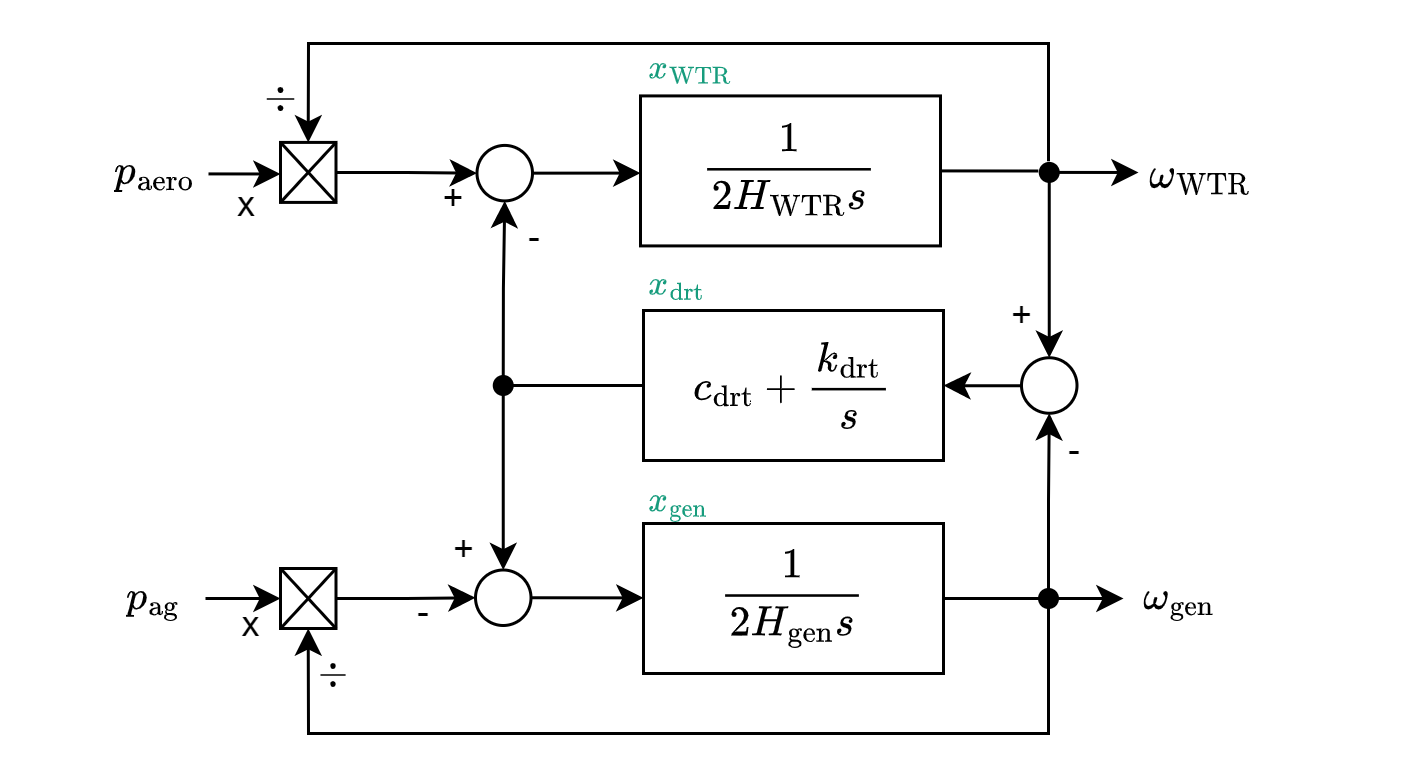
\includegraphics{drawings/WT_mechanical.drawio.png}

}

\caption{\label{fig-mechanicalModule}Wind turbine two mass mechanical
module, based on {[}1{]}}

\end{figure}%

\subsubsection{Parameters}\label{parameters-3}

\begin{longtable}[]{@{}
  >{\raggedright\arraybackslash}p{(\columnwidth - 10\tabcolsep) * \real{0.0600}}
  >{\raggedright\arraybackslash}p{(\columnwidth - 10\tabcolsep) * \real{0.0600}}
  >{\raggedright\arraybackslash}p{(\columnwidth - 10\tabcolsep) * \real{0.0500}}
  >{\raggedright\arraybackslash}p{(\columnwidth - 10\tabcolsep) * \real{0.2000}}
  >{\raggedright\arraybackslash}p{(\columnwidth - 10\tabcolsep) * \real{0.4400}}
  >{\raggedright\arraybackslash}p{(\columnwidth - 10\tabcolsep) * \real{0.0700}}@{}}
\caption{Parameters of mechanical moduele, based on {[}1{]} and
{[}8{]}}\label{tbl-parametersMechanical}\tabularnewline
\toprule\noalign{}
\begin{minipage}[b]{\linewidth}\raggedright
name
\end{minipage} & \begin{minipage}[b]{\linewidth}\raggedright
type
\end{minipage} & \begin{minipage}[b]{\linewidth}\raggedright
unit
\end{minipage} & \begin{minipage}[b]{\linewidth}\raggedright
base
\end{minipage} & \begin{minipage}[b]{\linewidth}\raggedright
description
\end{minipage} & \begin{minipage}[b]{\linewidth}\raggedright
typical value
\end{minipage} \\
\midrule\noalign{}
\endfirsthead
\toprule\noalign{}
\begin{minipage}[b]{\linewidth}\raggedright
name
\end{minipage} & \begin{minipage}[b]{\linewidth}\raggedright
type
\end{minipage} & \begin{minipage}[b]{\linewidth}\raggedright
unit
\end{minipage} & \begin{minipage}[b]{\linewidth}\raggedright
base
\end{minipage} & \begin{minipage}[b]{\linewidth}\raggedright
description
\end{minipage} & \begin{minipage}[b]{\linewidth}\raggedright
typical value
\end{minipage} \\
\midrule\noalign{}
\endhead
\bottomrule\noalign{}
\endlastfoot
\(c_\mathrm{drt}\) & float & pu &
\(T_\mathrm{base}/\Omega_\mathrm{base}\) & Damping of drive train &
2.344 \\
\(H_\mathrm{gen}\) & float & s & - & Inertia of generator rotor
(inertial time constant) & 3.395 \\
\(H_\mathrm{WTR}\) & float & s & - & Inertia of WT rotor (inertial time
constant) & 0.962 \\
\(k_\mathrm{drt}\) & float & pu & \(T_\mathrm{base}\) & Stiffness of
drive train & 1.378 \\
\end{longtable}

\subsubsection{Variables}\label{variables-4}

\paragraph{Inputs}\label{inputs-4}

\begin{longtable}[]{@{}
  >{\raggedright\arraybackslash}p{(\columnwidth - 8\tabcolsep) * \real{0.1589}}
  >{\raggedright\arraybackslash}p{(\columnwidth - 8\tabcolsep) * \real{0.0467}}
  >{\raggedright\arraybackslash}p{(\columnwidth - 8\tabcolsep) * \real{0.0374}}
  >{\raggedright\arraybackslash}p{(\columnwidth - 8\tabcolsep) * \real{0.1589}}
  >{\raggedright\arraybackslash}p{(\columnwidth - 8\tabcolsep) * \real{0.5981}}@{}}
\caption{Inputs, based on
{[}1{]}}\label{tbl-inputsMechanical}\tabularnewline
\toprule\noalign{}
\begin{minipage}[b]{\linewidth}\raggedright
name
\end{minipage} & \begin{minipage}[b]{\linewidth}\raggedright
type
\end{minipage} & \begin{minipage}[b]{\linewidth}\raggedright
unit
\end{minipage} & \begin{minipage}[b]{\linewidth}\raggedright
base
\end{minipage} & \begin{minipage}[b]{\linewidth}\raggedright
description
\end{minipage} \\
\midrule\noalign{}
\endfirsthead
\toprule\noalign{}
\begin{minipage}[b]{\linewidth}\raggedright
name
\end{minipage} & \begin{minipage}[b]{\linewidth}\raggedright
type
\end{minipage} & \begin{minipage}[b]{\linewidth}\raggedright
unit
\end{minipage} & \begin{minipage}[b]{\linewidth}\raggedright
base
\end{minipage} & \begin{minipage}[b]{\linewidth}\raggedright
description
\end{minipage} \\
\midrule\noalign{}
\endhead
\bottomrule\noalign{}
\endlastfoot
\(p_\mathrm{aero}\) & float & pu & \(S_\mathrm{base}\) & Aerodynamic
power (Power transferred from wind to WT rotor \\
\(p_\mathrm{ag}\) & float & pu & \(S_\mathrm{base}\) & Air gap power
(power transferred from generator rotor to stator) \\
\end{longtable}

\paragraph{Outputs}\label{outputs-4}

\begin{longtable}[]{@{}
  >{\raggedright\arraybackslash}p{(\columnwidth - 8\tabcolsep) * \real{0.2763}}
  >{\raggedright\arraybackslash}p{(\columnwidth - 8\tabcolsep) * \real{0.0658}}
  >{\raggedright\arraybackslash}p{(\columnwidth - 8\tabcolsep) * \real{0.0526}}
  >{\raggedright\arraybackslash}p{(\columnwidth - 8\tabcolsep) * \real{0.2895}}
  >{\raggedright\arraybackslash}p{(\columnwidth - 8\tabcolsep) * \real{0.3158}}@{}}
\caption{Outputs, based on
{[}1{]}}\label{tbl-outputsMechanical}\tabularnewline
\toprule\noalign{}
\begin{minipage}[b]{\linewidth}\raggedright
name
\end{minipage} & \begin{minipage}[b]{\linewidth}\raggedright
type
\end{minipage} & \begin{minipage}[b]{\linewidth}\raggedright
unit
\end{minipage} & \begin{minipage}[b]{\linewidth}\raggedright
base
\end{minipage} & \begin{minipage}[b]{\linewidth}\raggedright
description
\end{minipage} \\
\midrule\noalign{}
\endfirsthead
\toprule\noalign{}
\begin{minipage}[b]{\linewidth}\raggedright
name
\end{minipage} & \begin{minipage}[b]{\linewidth}\raggedright
type
\end{minipage} & \begin{minipage}[b]{\linewidth}\raggedright
unit
\end{minipage} & \begin{minipage}[b]{\linewidth}\raggedright
base
\end{minipage} & \begin{minipage}[b]{\linewidth}\raggedright
description
\end{minipage} \\
\midrule\noalign{}
\endhead
\bottomrule\noalign{}
\endlastfoot
\(\omega_\mathrm{gen}\) & float & pu & \(\Omega_\mathrm{base}\) &
generator rotor speed \\
\(\omega_\mathrm{WTR}\) & float & pu & \(\Omega_\mathrm{base}\) & Wind
turbine rotor speed \\
\end{longtable}

\subsubsection{Initial equations}\label{initial-equations-2}

For the used initialization helper variables, see
Section~\ref{sec-initHelpersGlobal}.

\begin{equation}\phantomsection\label{eq-initXwtr}{
x_\mathrm{WTR\,0} = x_\mathrm{gen\,0} = \omega_0
}\end{equation}

\begin{equation}\phantomsection\label{eq-initXdrt}{
x_\mathrm{drt\,0} = P_\mathrm{ag\,0} / \omega_0
}\end{equation}

\subsection{Two-dimensional aerodynamic module}\label{sec-aerodynamic2d}

The two-dimensional aerodynamic module is shown in
Figure~\ref{fig-wtAerodynamic}. \(\theta_0\) represents the rated pitch
angle (refers to the angle at which the turbine blades are positioned to
achieve maximum power output at a specific wind speed).

\begin{figure}

\centering{

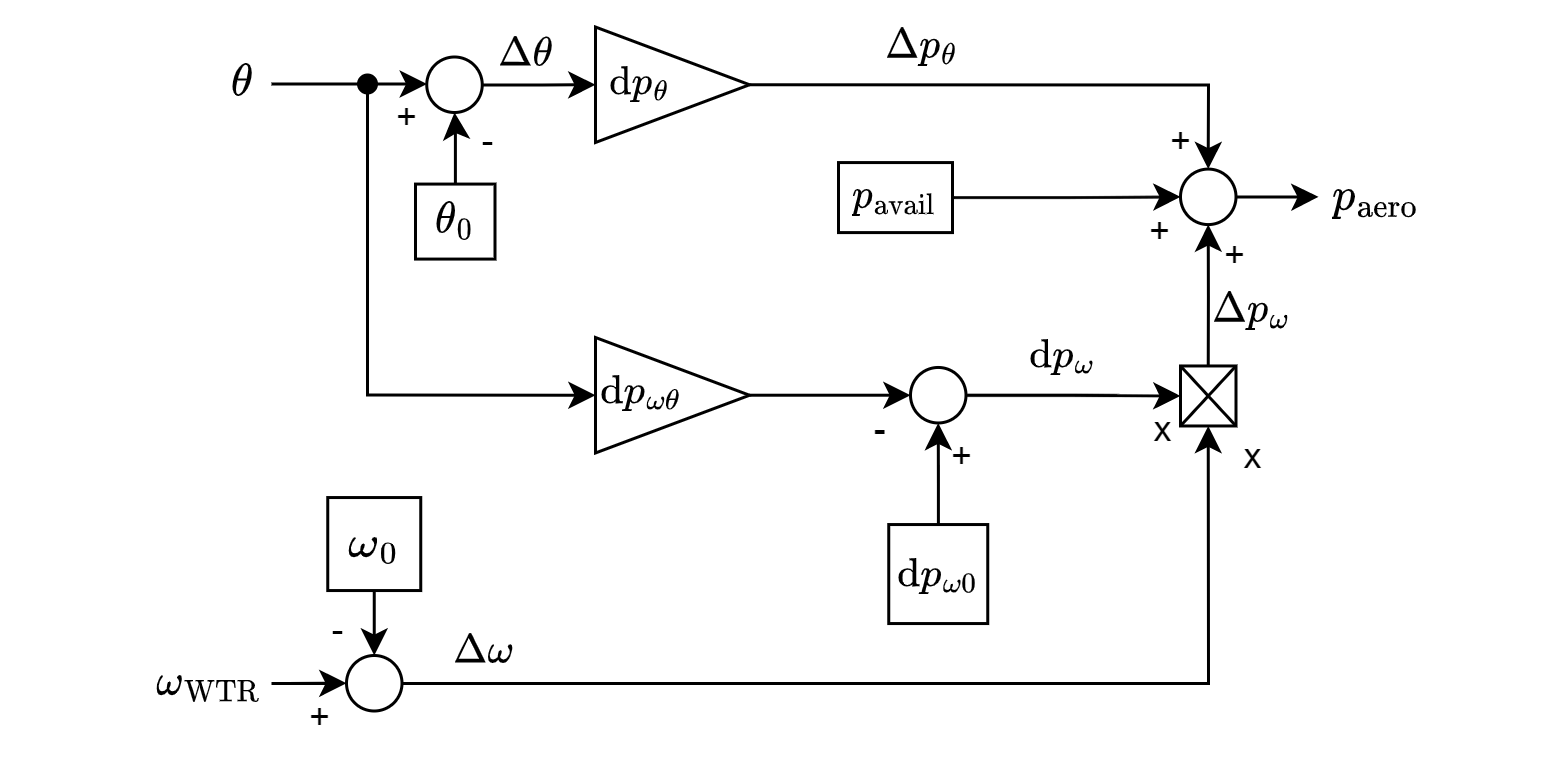
\includegraphics{drawings/WT_aerodynamic.drawio.png}

}

\caption{\label{fig-wtAerodynamic}Wind turbine two-dimensional
aerodynamic module (Type 3), based on {[}1{]}}

\end{figure}%

The rated pitch angle \(\theta_0\) is subtracted from the actual wind
turbine pitch angle \(\theta\) to obtain \(\Delta\theta\). The pitch
angle difference \(\Delta\theta\) is then multiplied by
\(\mathrm{d}p_{\theta}\) to compute \(\Delta p_\mathrm{\theta}\), the
change of aerodynamic power depending on the pitch angle change {[}3{]}.
\(\mathrm{d}p_{\theta}\) is the the aerodynamic power partial derivative
with respect to \(\theta\).

\(\Delta p_\mathrm{\theta}\) is typically negative because
\(\mathrm{d}p_{\theta}<0\) and represents power redution because of
pitch angle change. It is then added to the available power
\(p_\mathrm{avail}\), which depends on wind speed.

To get the speed-dependent component \(\Delta p_\mathrm{\omega}\), first
\(\Delta\omega\) is calculated from the wind turbine's reference speed
\(\omega_\mathrm{0}\) and the actual speed \(\omega_\mathrm{WTR}\).
\(\Delta\omega\) is then multiplied by \(\mathrm{d}p_\mathrm{\omega}\),
the aerodynamic power partial derivative with respect to \(\omega\).

\(\mathrm{d}p_\mathrm{\omega}\) is itself dependent on the pitch angle
\(\theta\), so it is calculated from \(\theta\),
\(\mathrm{d}p_\mathrm{\omega\theta}\) and
\(\mathrm{d}p_\mathrm{\omega0}\), where
\(\mathrm{d}p_\mathrm{\omega\theta}\) is the pitch-dependency of
\(\mathrm{d}p_\mathrm{\omega}\). \(\mathrm{d}p_{\omega0}\) is the
constant term of \(\mathrm{d}p_{\omega}\) and depends on the wind speed.

The resulting change \(\Delta p_\mathrm{\omega}\) of aerodynamic power
depending on rotor speed is added to \(p_\mathrm{avail}\) as well,
resulting in the wind turbine aerodynamic power \(p_\mathrm{aero}\)
{[}3{]}.

\subsubsection{Parameters}\label{parameters-4}

Typical values were gathered from the \emph{DIgSILENT PowerFactory}
implementation of the model.

\begin{longtable}[]{@{}
  >{\raggedright\arraybackslash}p{(\columnwidth - 12\tabcolsep) * \real{0.0600}}
  >{\raggedright\arraybackslash}p{(\columnwidth - 12\tabcolsep) * \real{0.0600}}
  >{\raggedright\arraybackslash}p{(\columnwidth - 12\tabcolsep) * \real{0.0500}}
  >{\raggedright\arraybackslash}p{(\columnwidth - 12\tabcolsep) * \real{0.1900}}
  >{\raggedright\arraybackslash}p{(\columnwidth - 12\tabcolsep) * \real{0.1900}}
  >{\raggedright\arraybackslash}p{(\columnwidth - 12\tabcolsep) * \real{0.4100}}
  >{\raggedleft\arraybackslash}p{(\columnwidth - 12\tabcolsep) * \real{0.0700}}@{}}
\caption{Parameters, based on
{[}1{]}}\label{tbl-parametersAero}\tabularnewline
\toprule\noalign{}
\begin{minipage}[b]{\linewidth}\raggedright
name
\end{minipage} & \begin{minipage}[b]{\linewidth}\raggedright
type
\end{minipage} & \begin{minipage}[b]{\linewidth}\raggedright
unit
\end{minipage} & \begin{minipage}[b]{\linewidth}\raggedright
base
\end{minipage} & \begin{minipage}[b]{\linewidth}\raggedright
modelica name
\end{minipage} & \begin{minipage}[b]{\linewidth}\raggedright
description
\end{minipage} & \begin{minipage}[b]{\linewidth}\raggedleft
typical values
\end{minipage} \\
\midrule\noalign{}
\endfirsthead
\toprule\noalign{}
\begin{minipage}[b]{\linewidth}\raggedright
name
\end{minipage} & \begin{minipage}[b]{\linewidth}\raggedright
type
\end{minipage} & \begin{minipage}[b]{\linewidth}\raggedright
unit
\end{minipage} & \begin{minipage}[b]{\linewidth}\raggedright
base
\end{minipage} & \begin{minipage}[b]{\linewidth}\raggedright
modelica name
\end{minipage} & \begin{minipage}[b]{\linewidth}\raggedright
description
\end{minipage} & \begin{minipage}[b]{\linewidth}\raggedleft
typical values
\end{minipage} \\
\midrule\noalign{}
\endhead
\bottomrule\noalign{}
\endlastfoot
\(\mathrm{d}p_\mathrm{\omega 0}\) & float & pu &
\(S_{\mathrm{base}} / \Omega_{\mathrm{base}}\) & DPOmega0Pu & Constant
term of aerodynamic power partial derivative with respect to wind
turbine rotor speed & 0.48 \\
\(\mathrm{d}p_\mathrm{\omega \theta}\) & float & pu &
\(S_{\mathrm{base}} / \Omega_{\mathrm{base}} / \mathrm{deg}\) &
DPOmegaThetaPu & Pitch dependency of aerodynamic power partial
derivative with respect to wind turbine rotor speed & 0.028 \\
\(\mathrm{d}p_\mathrm{\theta}\) & float & pu &
\(S_{\mathrm{base}} / \mathrm{deg}\) & DPThetaPu & Aerodynamic power
partial derivative with respect to pitch angle (usually \(<0\)) &
-0.03 \\
\(\omega_0\) & float & pu & \(\Omega_{\mathrm{base}}\) & Omega0Pu &
Rotor speed of the wind turbine, if not derated & 1 \\
\(p_{\mathrm{avail}}\) & float & pu & \(S_{\mathrm{base}}\) & PAvailPu &
Available power; \(p_\mathrm{aero}\) cannot be greater than
\(p_\mathrm{avail}\) & 1 \\
\(\theta_0\) & float & deg & deg & Theta0 & Pitch angle of the wind
turbine in maximum available power operation & 0 \\
\end{longtable}

\begin{tcolorbox}[enhanced jigsaw, coltitle=black, bottomrule=.15mm, opacitybacktitle=0.6, rightrule=.15mm, colframe=quarto-callout-note-color-frame, titlerule=0mm, arc=.35mm, breakable, colbacktitle=quarto-callout-note-color!10!white, title=\textcolor{quarto-callout-note-color}{\faInfo}\hspace{0.5em}{Note}, colback=white, bottomtitle=1mm, toprule=.15mm, leftrule=.75mm, toptitle=1mm, left=2mm, opacityback=0]

According to {[}1{]}, for \(0 < p_\mathrm{avail} < 1\) the pitch angle
should be zero. It should be greater than zero if
\(p_\mathrm{avail} = 1\) or if the initial value of \(p_\mathrm{aero}\)
is less than \(p_\mathrm{avail}\).

\end{tcolorbox}

\subsubsection{Variables}\label{variables-5}

\paragraph{Inputs}\label{inputs-5}

\begin{longtable}[]{@{}
  >{\raggedright\arraybackslash}p{(\columnwidth - 10\tabcolsep) * \real{0.0600}}
  >{\raggedright\arraybackslash}p{(\columnwidth - 10\tabcolsep) * \real{0.0600}}
  >{\raggedright\arraybackslash}p{(\columnwidth - 10\tabcolsep) * \real{0.0500}}
  >{\raggedright\arraybackslash}p{(\columnwidth - 10\tabcolsep) * \real{0.2000}}
  >{\raggedright\arraybackslash}p{(\columnwidth - 10\tabcolsep) * \real{0.1500}}
  >{\raggedright\arraybackslash}p{(\columnwidth - 10\tabcolsep) * \real{0.4400}}@{}}
\caption{Inputs, based on {[}1{]}}\label{tbl-inputsAero}\tabularnewline
\toprule\noalign{}
\begin{minipage}[b]{\linewidth}\raggedright
name
\end{minipage} & \begin{minipage}[b]{\linewidth}\raggedright
type
\end{minipage} & \begin{minipage}[b]{\linewidth}\raggedright
unit
\end{minipage} & \begin{minipage}[b]{\linewidth}\raggedright
base
\end{minipage} & \begin{minipage}[b]{\linewidth}\raggedright
modelica name
\end{minipage} & \begin{minipage}[b]{\linewidth}\raggedright
description
\end{minipage} \\
\midrule\noalign{}
\endfirsthead
\toprule\noalign{}
\begin{minipage}[b]{\linewidth}\raggedright
name
\end{minipage} & \begin{minipage}[b]{\linewidth}\raggedright
type
\end{minipage} & \begin{minipage}[b]{\linewidth}\raggedright
unit
\end{minipage} & \begin{minipage}[b]{\linewidth}\raggedright
base
\end{minipage} & \begin{minipage}[b]{\linewidth}\raggedright
modelica name
\end{minipage} & \begin{minipage}[b]{\linewidth}\raggedright
description
\end{minipage} \\
\midrule\noalign{}
\endhead
\bottomrule\noalign{}
\endlastfoot
\(\omega_\mathrm{WTR}\) & float & pu & \(\Omega_{\mathrm{base}}\) &
omegaWTRPu & Wind Turbine Rotor speed \\
\(\theta\) & float & deg & Deg & theta & Wind Turbine Pitch angle \\
\end{longtable}

\paragraph{Outputs}\label{outputs-5}

\begin{longtable}[]{@{}
  >{\raggedright\arraybackslash}p{(\columnwidth - 10\tabcolsep) * \real{0.0600}}
  >{\raggedright\arraybackslash}p{(\columnwidth - 10\tabcolsep) * \real{0.0600}}
  >{\raggedright\arraybackslash}p{(\columnwidth - 10\tabcolsep) * \real{0.0500}}
  >{\raggedright\arraybackslash}p{(\columnwidth - 10\tabcolsep) * \real{0.2000}}
  >{\raggedright\arraybackslash}p{(\columnwidth - 10\tabcolsep) * \real{0.1000}}
  >{\raggedright\arraybackslash}p{(\columnwidth - 10\tabcolsep) * \real{0.4400}}@{}}
\caption{Outputs, based on
{[}1{]}}\label{tbl-outputsAero}\tabularnewline
\toprule\noalign{}
\begin{minipage}[b]{\linewidth}\raggedright
name
\end{minipage} & \begin{minipage}[b]{\linewidth}\raggedright
type
\end{minipage} & \begin{minipage}[b]{\linewidth}\raggedright
unit
\end{minipage} & \begin{minipage}[b]{\linewidth}\raggedright
base
\end{minipage} & \begin{minipage}[b]{\linewidth}\raggedright
modelica name
\end{minipage} & \begin{minipage}[b]{\linewidth}\raggedright
description
\end{minipage} \\
\midrule\noalign{}
\endfirsthead
\toprule\noalign{}
\begin{minipage}[b]{\linewidth}\raggedright
name
\end{minipage} & \begin{minipage}[b]{\linewidth}\raggedright
type
\end{minipage} & \begin{minipage}[b]{\linewidth}\raggedright
unit
\end{minipage} & \begin{minipage}[b]{\linewidth}\raggedright
base
\end{minipage} & \begin{minipage}[b]{\linewidth}\raggedright
modelica name
\end{minipage} & \begin{minipage}[b]{\linewidth}\raggedright
description
\end{minipage} \\
\midrule\noalign{}
\endhead
\bottomrule\noalign{}
\endlastfoot
\(p_\mathrm{aero}\) & float & & Deg & pAeroPu & Wind Turbine aerodynamic
power \\
\end{longtable}

\subsection{Pitch angle control
module}\label{pitch-angle-control-module}

\begin{figure}

\centering{

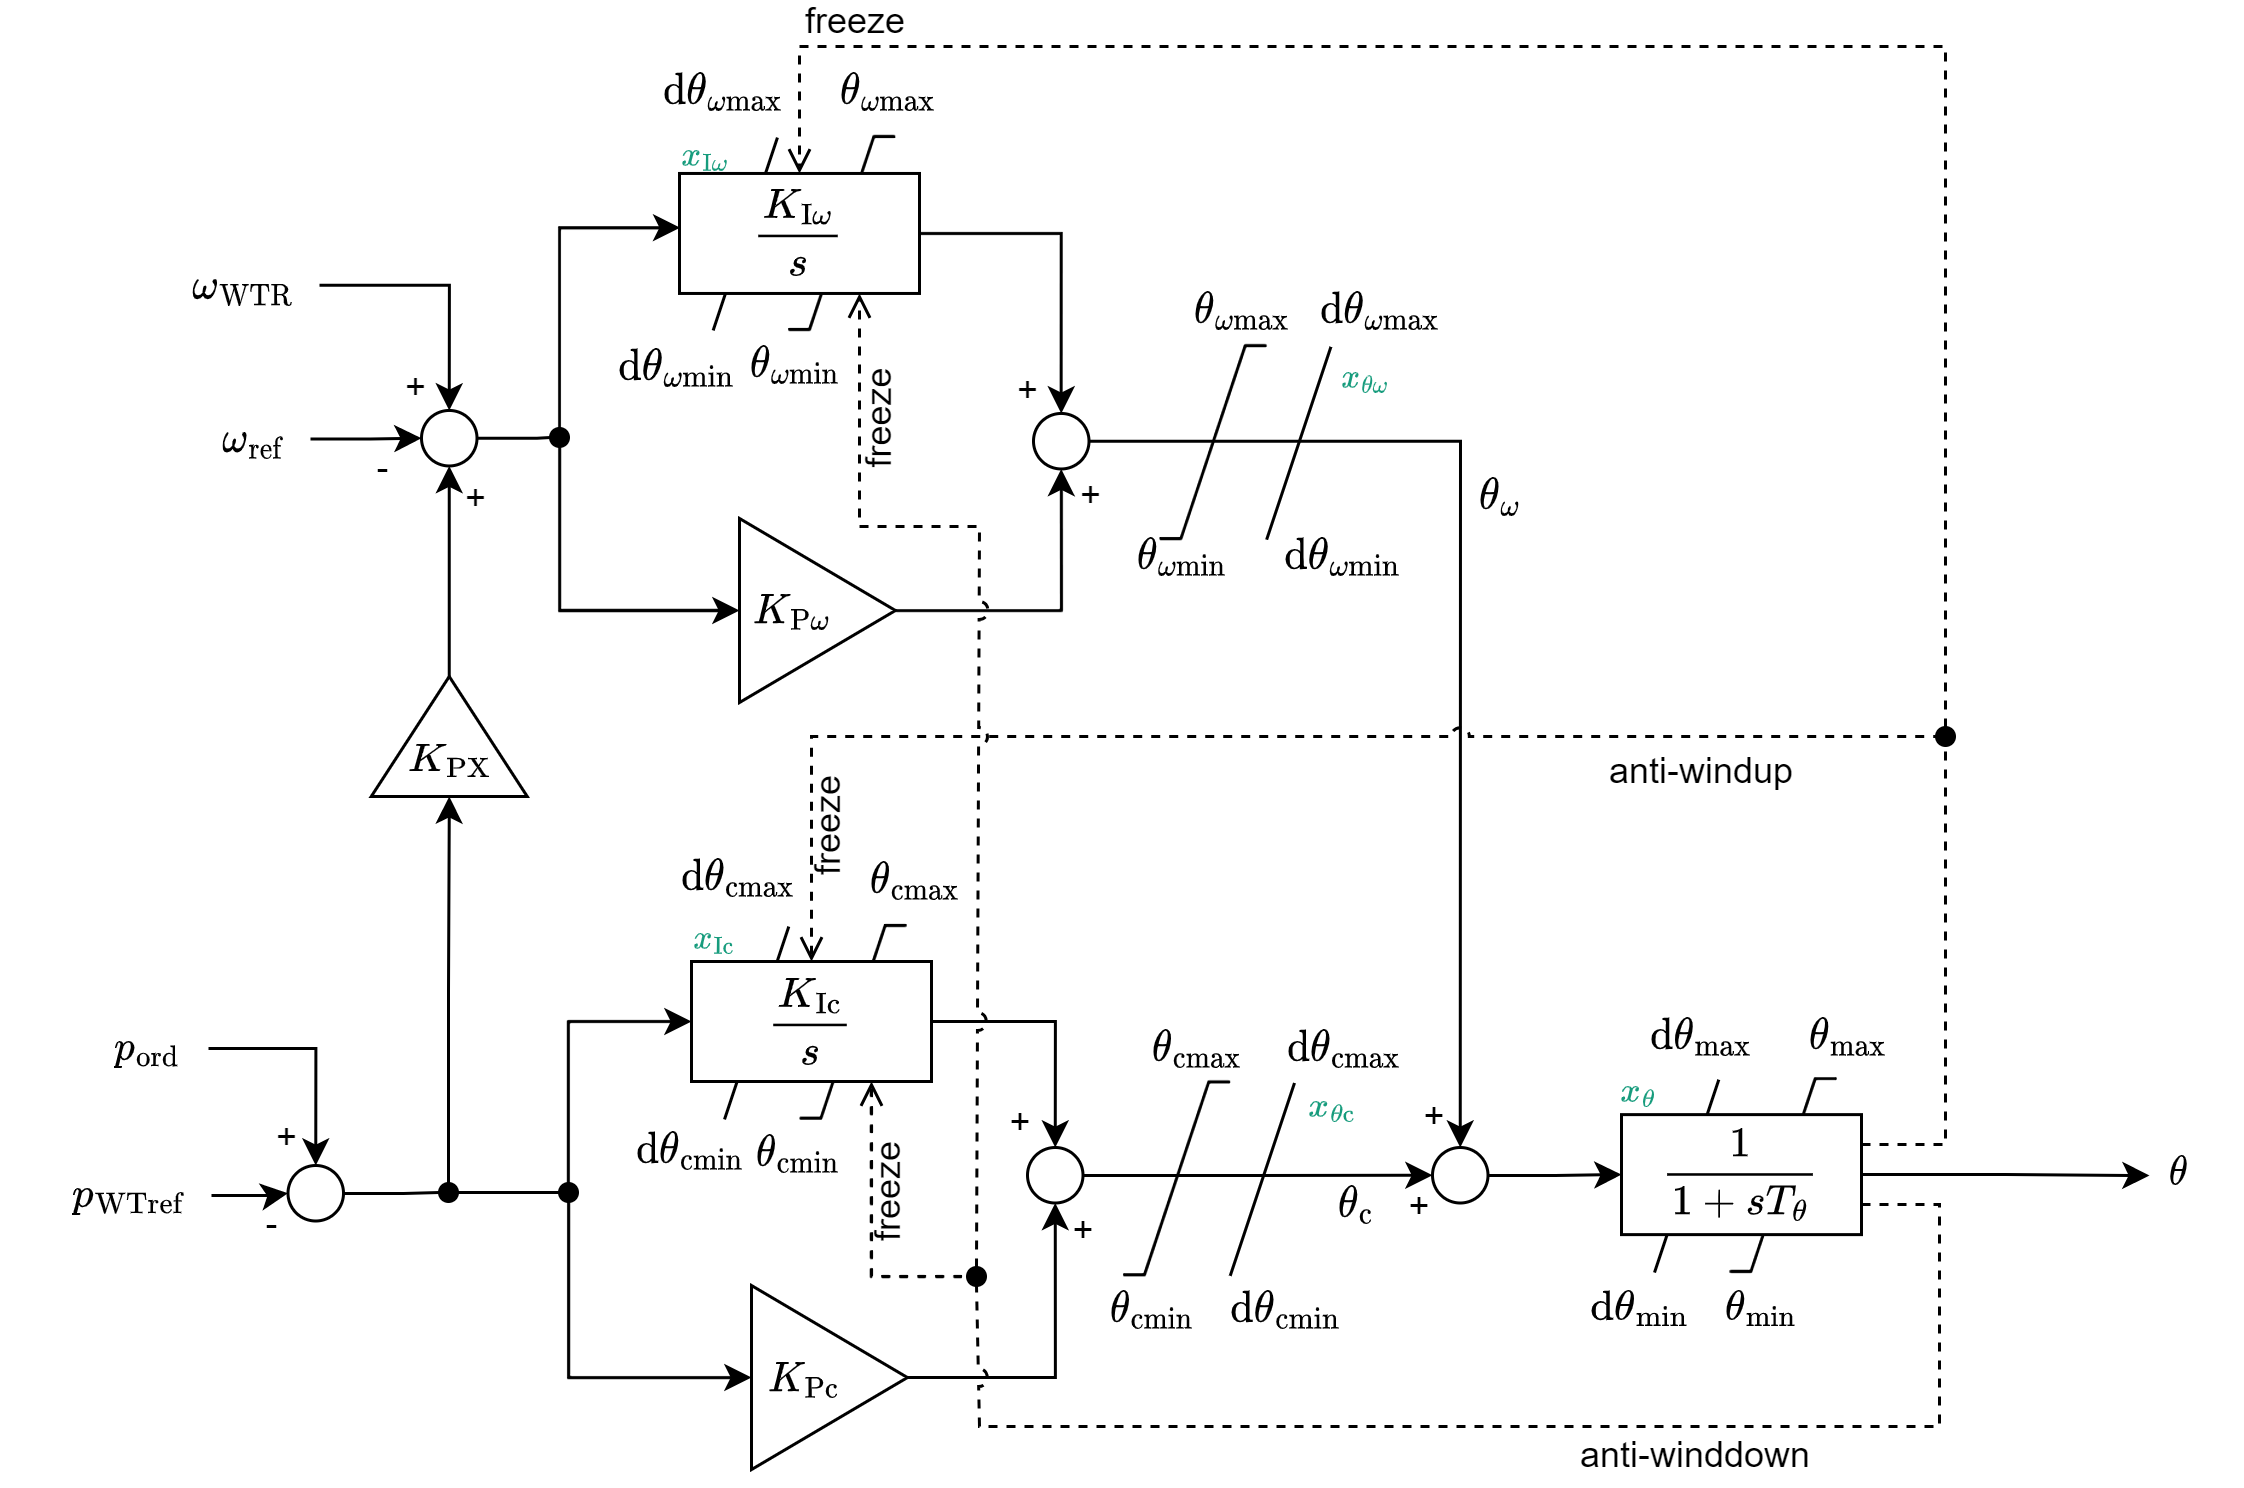
\includegraphics{drawings/WT_pitch.drawio.png}

}

\caption{\label{fig-wtPitchAngleControl}Wind turbine pitch angle module
(Type 3), based on {[}1{]}}

\end{figure}%

The pitch angle control module is shown in
Figure~\ref{fig-wtPitchAngleControl}. It uses two PI controllers to
control the pitch angle \(\theta\), one associated with rotor speed
(\(K_\mathrm{I\omega}\), \(K_\mathrm{P\omega}\)) and one with generator
power (\(K_\mathrm{Ic}\), \(K_\mathrm{Pc}\)) {[}2{]}.

The outputs of both PI controllers are pitch angle setpoints
(\(\theta_\mathrm{\omega}\) and \(\theta_\mathrm{c}\)). They are kept
inside their respective limits (\(\theta_\mathrm{\omega min|max}\) and
\(\theta_\mathrm{cmin|max}\)), similarly for the pitch angles' rates of
change.

The rotor speed and power integrators are anti-windup, which means that
the integrator is blocked when the lower or upper limit of \(\theta\)
are reached, until the error input changes direction. Both controller
outputs are added before a low-pass filter (time constant \(T_\theta\))
is applied. The filter with limitation detection considers the pitch
angle limitation \(\theta_\mathrm{min|max}\) and pitch angle rate of
change \(\mathrm{d}\theta_{\mathrm{min|max}}\).

The pitch angle rate of change plays a crucial role during power system
faults since it avoids overspeeding during faults by controlling how
fast the aerodynamic power is reduced {[}2{]}.

Since a Doubly-Fed Induction Generator (DFIG) turbine is already
operating at rated rotor speed before reaching nominal wind speed, under
certain conditions, the pitch (\(\theta\) \textgreater{} 0) could be
activated even though the generated active power is lower than 1 pu.
Therefore, the cross-coupling gain \(K_\mathrm{PX}\) is used to modify
the signal introduced into the rotor speed error {[}2{]}.

\subsubsection{Parameters}\label{parameters-5}

Typical values were gathered from the \emph{DIgSILENT PowerFactory}
implementation of the model.

\begin{longtable}[]{@{}
  >{\raggedright\arraybackslash}p{(\columnwidth - 12\tabcolsep) * \real{0.0600}}
  >{\raggedright\arraybackslash}p{(\columnwidth - 12\tabcolsep) * \real{0.0600}}
  >{\raggedright\arraybackslash}p{(\columnwidth - 12\tabcolsep) * \real{0.0500}}
  >{\raggedright\arraybackslash}p{(\columnwidth - 12\tabcolsep) * \real{0.1600}}
  >{\raggedright\arraybackslash}p{(\columnwidth - 12\tabcolsep) * \real{0.1900}}
  >{\raggedright\arraybackslash}p{(\columnwidth - 12\tabcolsep) * \real{0.4200}}
  >{\raggedright\arraybackslash}p{(\columnwidth - 12\tabcolsep) * \real{0.0700}}@{}}
\caption{Parameters, based on
{[}1{]}}\label{tbl-parametersPitch}\tabularnewline
\toprule\noalign{}
\begin{minipage}[b]{\linewidth}\raggedright
name
\end{minipage} & \begin{minipage}[b]{\linewidth}\raggedright
type
\end{minipage} & \begin{minipage}[b]{\linewidth}\raggedright
unit
\end{minipage} & \begin{minipage}[b]{\linewidth}\raggedright
base
\end{minipage} & \begin{minipage}[b]{\linewidth}\raggedright
modelica name
\end{minipage} & \begin{minipage}[b]{\linewidth}\raggedright
description
\end{minipage} & \begin{minipage}[b]{\linewidth}\raggedright
typical values
\end{minipage} \\
\midrule\noalign{}
\endfirsthead
\toprule\noalign{}
\begin{minipage}[b]{\linewidth}\raggedright
name
\end{minipage} & \begin{minipage}[b]{\linewidth}\raggedright
type
\end{minipage} & \begin{minipage}[b]{\linewidth}\raggedright
unit
\end{minipage} & \begin{minipage}[b]{\linewidth}\raggedright
base
\end{minipage} & \begin{minipage}[b]{\linewidth}\raggedright
modelica name
\end{minipage} & \begin{minipage}[b]{\linewidth}\raggedright
description
\end{minipage} & \begin{minipage}[b]{\linewidth}\raggedright
typical values
\end{minipage} \\
\midrule\noalign{}
\endhead
\bottomrule\noalign{}
\endlastfoot
\(\mathrm{d}\theta_{\mathrm{cmax}}\) & float & deg/s & - & DThetaCmax &
Pitch maximum positive ramp rate of power PI controller & 6 \\
\(\mathrm{d}\theta_{\mathrm{cmin}}\) & float & deg/s & - & DThetaCmin &
Pitch minimum positive ramp rate of power PI controllerr & -3 \\
\(\mathrm{d}\theta_{\mathrm{max}}\) & float & deg/s & - & DThetaMax &
Pitch maximum positive ramp rate & 6 \\
\(\mathrm{d}\theta_{\mathrm{min}}\) & float & deg/s & - & DThetaMin &
Pitch maximum negative ramp rate & -3 \\
\(\mathrm{d}\theta_{\omega\mathrm{max}}\) & float & deg/s & - &
DThetaOmegamax & Pitch maximum positive ramp rate of speed PI controller
& 6 \\
\(\mathrm{d}\theta_{\omega\mathrm{min}}\) & float & deg/s & - &
DThetaOmegamin & Pitch maximum negative ramp rate of speed PI controller
& -3 \\
\(K_\mathrm{Ic}\) & float & pu &
\(\mathrm{deg} / S_{\mathrm{base}} / \mathrm{s}\) & KIcPu & Integration
gain of power PI controller & 0.0 \\
\(K_\mathrm{I\omega}\) & float & pu &
\(\mathrm{deg} / \Omega_{\mathrm{base}} / \mathrm{s}\) & KIOmegaPu &
Integration gain of speed PI controller & 15 \\
\(K_\mathrm{Pc}\) & float & pu & \(\mathrm{deg} / S_{\mathrm{base}}\) &
KPcPu & Proportional gain of power PI controller & 0 \\
\(K_\mathrm{P\omega}\) & float & pu &
\(\mathrm{deg} / \Omega_{\mathrm{base}}\) & KPomegaPu & Proportional
gain of speed PI controller & 15 \\
\(K_\mathrm{PX}\) & float & pu &
\(\Omega_{\mathrm{base}} / S_{\mathrm{base}}\) & KPXPu & Cross coupling
pitch gain & 0.03 \\
\(\theta_\mathrm{cmax}\) & float & deg & - & ThetaCmax & Maximum WT
pitch angle of power PI controller & 35 \\
\(\theta_\mathrm{cmin}\) & float & deg & - & ThetaCmin & Minimum WT
pitch angle of power PI controller & 0 \\
\(\theta_\mathrm{max}\) & float & deg & - & ThetaMax & Maximum WT pitch
angle & 35 \\
\(\theta_\mathrm{min}\) & float & deg & - & ThetaMin & Minimum WT pitch
angle & 0 \\
\(\theta_\mathrm{\omega max}\) & float & deg & - & ThetaOmegamax &
Maximum WT pitch angle of speed PI controller & 35 \\
\(\theta_\mathrm{\omega min}\) & float & deg & - & ThetaOmegamin &
Minimum WT pitch angle of speed PI controller & 0 \\
\(T_\theta\) & float & s & - & TTheta & WT pitch time constant & 0.25 \\
\end{longtable}

\paragraph{Variables}\label{variables-6}

\subparagraph{Inputs}\label{inputs-6}

\begin{longtable}[]{@{}
  >{\raggedright\arraybackslash}p{(\columnwidth - 10\tabcolsep) * \real{0.0600}}
  >{\raggedright\arraybackslash}p{(\columnwidth - 10\tabcolsep) * \real{0.0600}}
  >{\raggedright\arraybackslash}p{(\columnwidth - 10\tabcolsep) * \real{0.0500}}
  >{\raggedright\arraybackslash}p{(\columnwidth - 10\tabcolsep) * \real{0.0700}}
  >{\raggedright\arraybackslash}p{(\columnwidth - 10\tabcolsep) * \real{0.1500}}
  >{\raggedright\arraybackslash}p{(\columnwidth - 10\tabcolsep) * \real{0.4400}}@{}}
\caption{Inputs, based on {[}1{]}}\label{tbl-inputsPitch}\tabularnewline
\toprule\noalign{}
\begin{minipage}[b]{\linewidth}\raggedright
name
\end{minipage} & \begin{minipage}[b]{\linewidth}\raggedright
type
\end{minipage} & \begin{minipage}[b]{\linewidth}\raggedright
unit
\end{minipage} & \begin{minipage}[b]{\linewidth}\raggedright
base
\end{minipage} & \begin{minipage}[b]{\linewidth}\raggedright
modelica name
\end{minipage} & \begin{minipage}[b]{\linewidth}\raggedright
description
\end{minipage} \\
\midrule\noalign{}
\endfirsthead
\toprule\noalign{}
\begin{minipage}[b]{\linewidth}\raggedright
name
\end{minipage} & \begin{minipage}[b]{\linewidth}\raggedright
type
\end{minipage} & \begin{minipage}[b]{\linewidth}\raggedright
unit
\end{minipage} & \begin{minipage}[b]{\linewidth}\raggedright
base
\end{minipage} & \begin{minipage}[b]{\linewidth}\raggedright
modelica name
\end{minipage} & \begin{minipage}[b]{\linewidth}\raggedright
description
\end{minipage} \\
\midrule\noalign{}
\endhead
\bottomrule\noalign{}
\endlastfoot
\(\omega_\mathrm{ref}\) & float & pu & \(\Omega_\mathrm{base}\) &
omegaRefPu & Wind Turbine rotor speed reference \\
\(\omega_\mathrm{WTR}\) & float & pu & \(\Omega_\mathrm{base}\) &
omegaWTRPu & Wind Turbine rotor speed \\
\(p_\mathrm{ord}\) & float & pu & \(S_\mathrm{base}\) & pOrdPu & Wind
Turbine active power \\
\(p_\mathrm{WTref}\) & float & pu & \(S_\mathrm{base}\) & pWTrefPu &
Wind Turbine active power reference \\
\end{longtable}

\subparagraph{Outputs}\label{outputs-6}

\begin{longtable}[]{@{}
  >{\raggedright\arraybackslash}p{(\columnwidth - 10\tabcolsep) * \real{0.0600}}
  >{\raggedright\arraybackslash}p{(\columnwidth - 10\tabcolsep) * \real{0.0600}}
  >{\raggedright\arraybackslash}p{(\columnwidth - 10\tabcolsep) * \real{0.0500}}
  >{\raggedright\arraybackslash}p{(\columnwidth - 10\tabcolsep) * \real{0.2000}}
  >{\raggedright\arraybackslash}p{(\columnwidth - 10\tabcolsep) * \real{0.1000}}
  >{\raggedright\arraybackslash}p{(\columnwidth - 10\tabcolsep) * \real{0.4400}}@{}}
\caption{Outputs, based on
{[}1{]}}\label{tbl-outputsPitch}\tabularnewline
\toprule\noalign{}
\begin{minipage}[b]{\linewidth}\raggedright
name
\end{minipage} & \begin{minipage}[b]{\linewidth}\raggedright
type
\end{minipage} & \begin{minipage}[b]{\linewidth}\raggedright
unit
\end{minipage} & \begin{minipage}[b]{\linewidth}\raggedright
base
\end{minipage} & \begin{minipage}[b]{\linewidth}\raggedright
modelica name
\end{minipage} & \begin{minipage}[b]{\linewidth}\raggedright
description
\end{minipage} \\
\midrule\noalign{}
\endfirsthead
\toprule\noalign{}
\begin{minipage}[b]{\linewidth}\raggedright
name
\end{minipage} & \begin{minipage}[b]{\linewidth}\raggedright
type
\end{minipage} & \begin{minipage}[b]{\linewidth}\raggedright
unit
\end{minipage} & \begin{minipage}[b]{\linewidth}\raggedright
base
\end{minipage} & \begin{minipage}[b]{\linewidth}\raggedright
modelica name
\end{minipage} & \begin{minipage}[b]{\linewidth}\raggedright
description
\end{minipage} \\
\midrule\noalign{}
\endhead
\bottomrule\noalign{}
\endlastfoot
\(\theta\) & float & deg & - & theta & Wind Turbine pitch angle \\
\end{longtable}

\subsubsection{Initial equations}\label{initial-equations-3}

For the used initialization helper variables, see
Section~\ref{sec-initHelpersGlobal}.

For the used parameters of the aerodynamic module, see
Section~\ref{sec-aerodynamic2d}

\begin{equation}\phantomsection\label{eq-initIomega}{ 
x_\mathrm{I\omega} = x_\mathrm{\theta \omega} = x_\mathrm{\theta} = \theta_0 + (P_\mathrm{ag\,0}-p_\mathrm{avail})/\mathrm{d}p_\mathrm{\theta}
}\end{equation}

\begin{equation}\phantomsection\label{eq-initIc}{
x_\mathrm{Ic} = x_\mathrm{\theta c} = 0
}\end{equation}

\subsection{Generator system type 3}\label{generator-system-type-3}

\subsubsection{Description}\label{description}

Two different models (3A and 3B) have been definded in the IEC {[}1{]},
depending on the FRT solution implemented for the WT.

FRT implies large currents in the rotor and large power injected into
the DC circuit of the converter {[}2{]}. Rotor and converter protection
against high currents and voltages is realized by a DC chopper and/or an
AC crowbar circuit.

\textbf{A DC chopper} basically keeps the DC voltage constant by
dissipating energy through a switched resistor. This implies
controllability of the rotor by the converter during FRT.

\textbf{A crowbar circuit} consists of switchable resistances between
the rotor's phases. In case of undesirably high currents in the machine
rotor or high DC voltages, the crowbar switches are closed and the
rotor's windings short-circuited through the crowbar resistances. This
way, overcurrents and -voltages are prevented but there is no control
action by the converter on the rotor windings anymore and the generator
acts like a conventional slip-ring induction machine (Type 1 machine)
{[}4{]}. This leads to a delay on the delivery of voltage control
functionality as well as active and reactive power transients after
fault inception and fault clearance {[}2{]}.

\paragraph{Type 3A}\label{type-3a}

\begin{figure}

\centering{

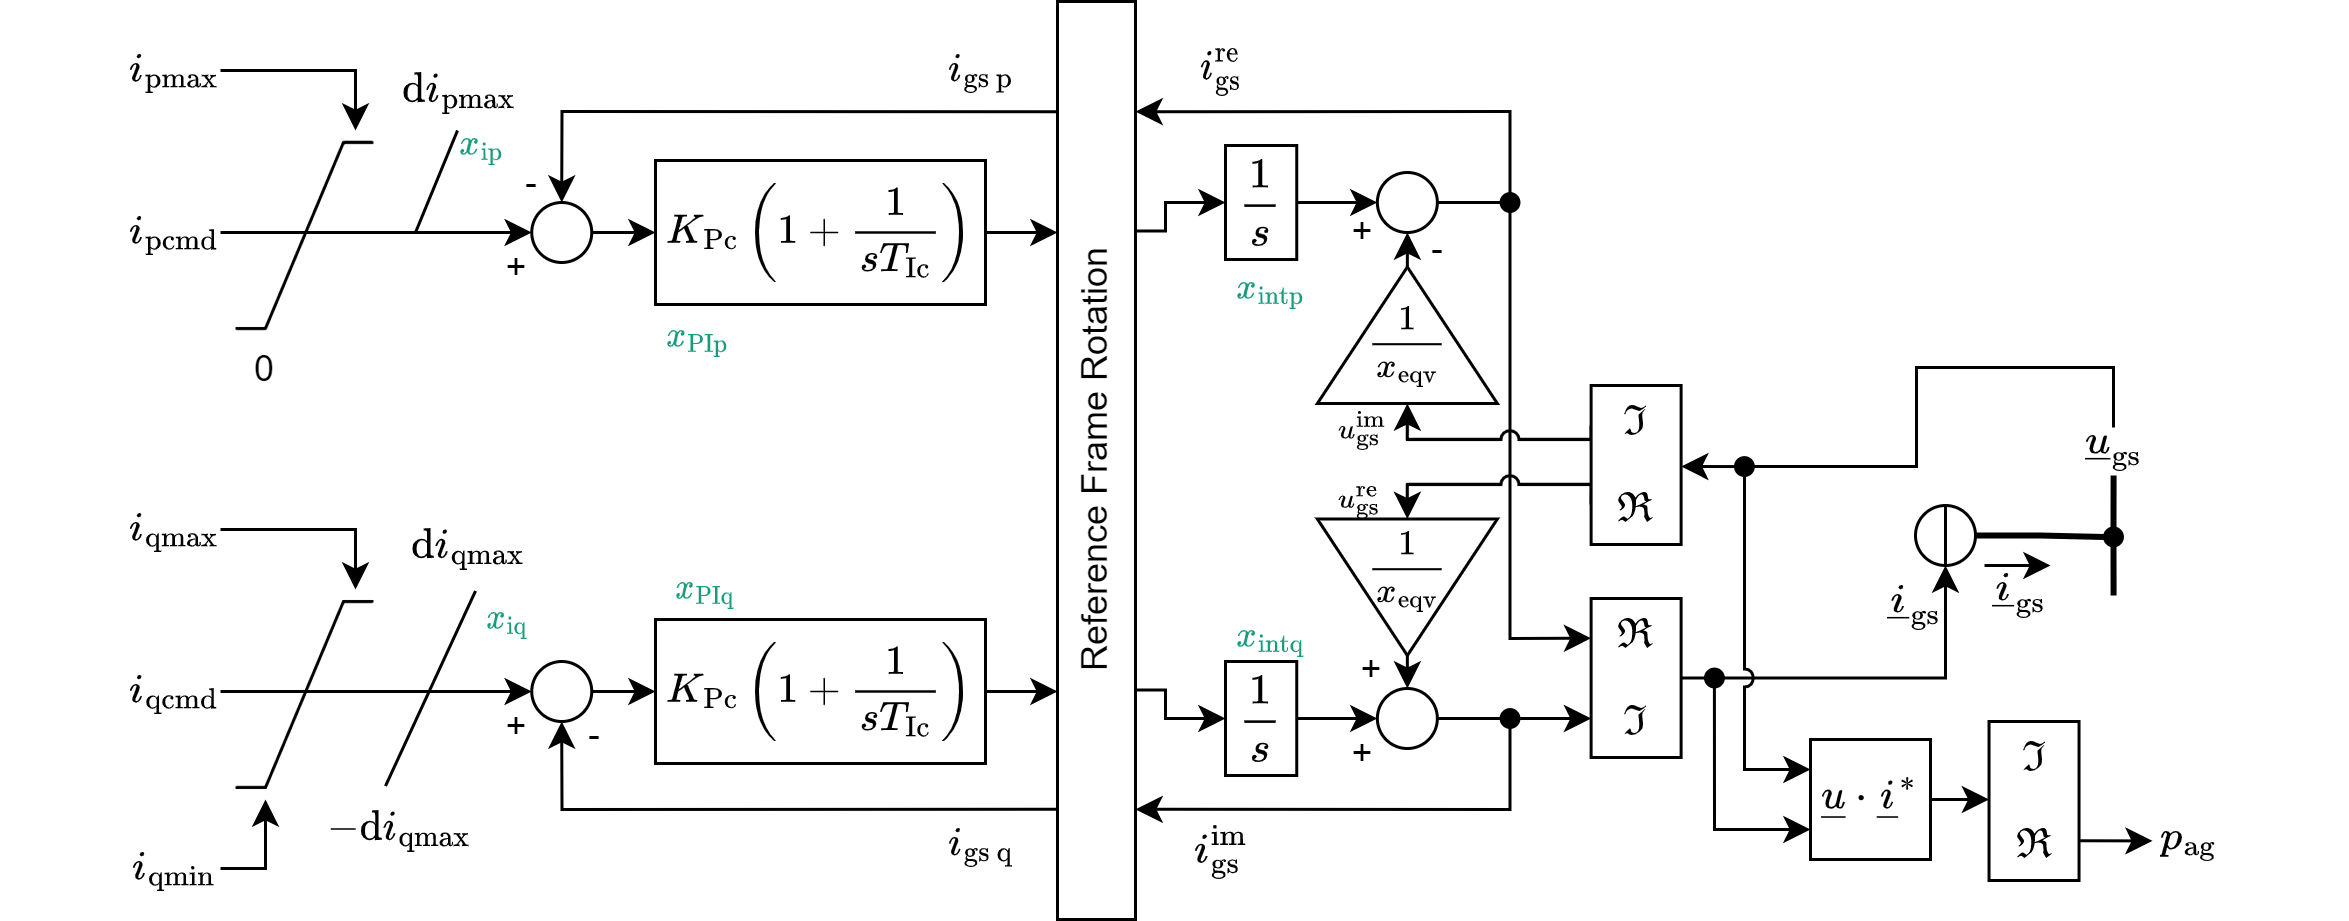
\includegraphics{drawings/WT_GS_3A.drawio.png}

}

\caption{\label{fig-generatorType3a}Wind turbine type 3A generator
system model, based on {[}1{]}}

\end{figure}%

The Type 3A Generator System represents a DFIG. Inside the WT controls,
\(i_\mathrm{p}\) and \(i_\mathrm{q}\) represent active and reactive
current components. On the grid side (gs), after the reference frame
rotation, this is not the case, because the voltage angle is different.
Hence, the PI current controller's output as well as the feedback of the
generator system's current need to be rotated in either direction to
match the respective reference frames.

Because the stator is directly coupled to the grid in case of a DFIG, an
abrupt voltage variation will cause a change in the reactive power flow.
The addition/subtraction of \(u / x_\mathrm{eqv}\) is added to simulate
these electromagnetic transients (related to rotor flux derivative)
{[}2{]} {[}6{]}.

The air-gap power \(p_\mathrm{ag}\) is an additional output of the
model, which is used as an input for the mechanical model in
Figure~\ref{fig-mechanicalModule}.

In this model a DC chopper is assumed. The model is not applicable for
older DFIG systems that require a crowbar during grid faults ({[}3{]},
p.~111).

\paragraph{Type 3B}\label{type-3b}

\begin{figure}

\centering{

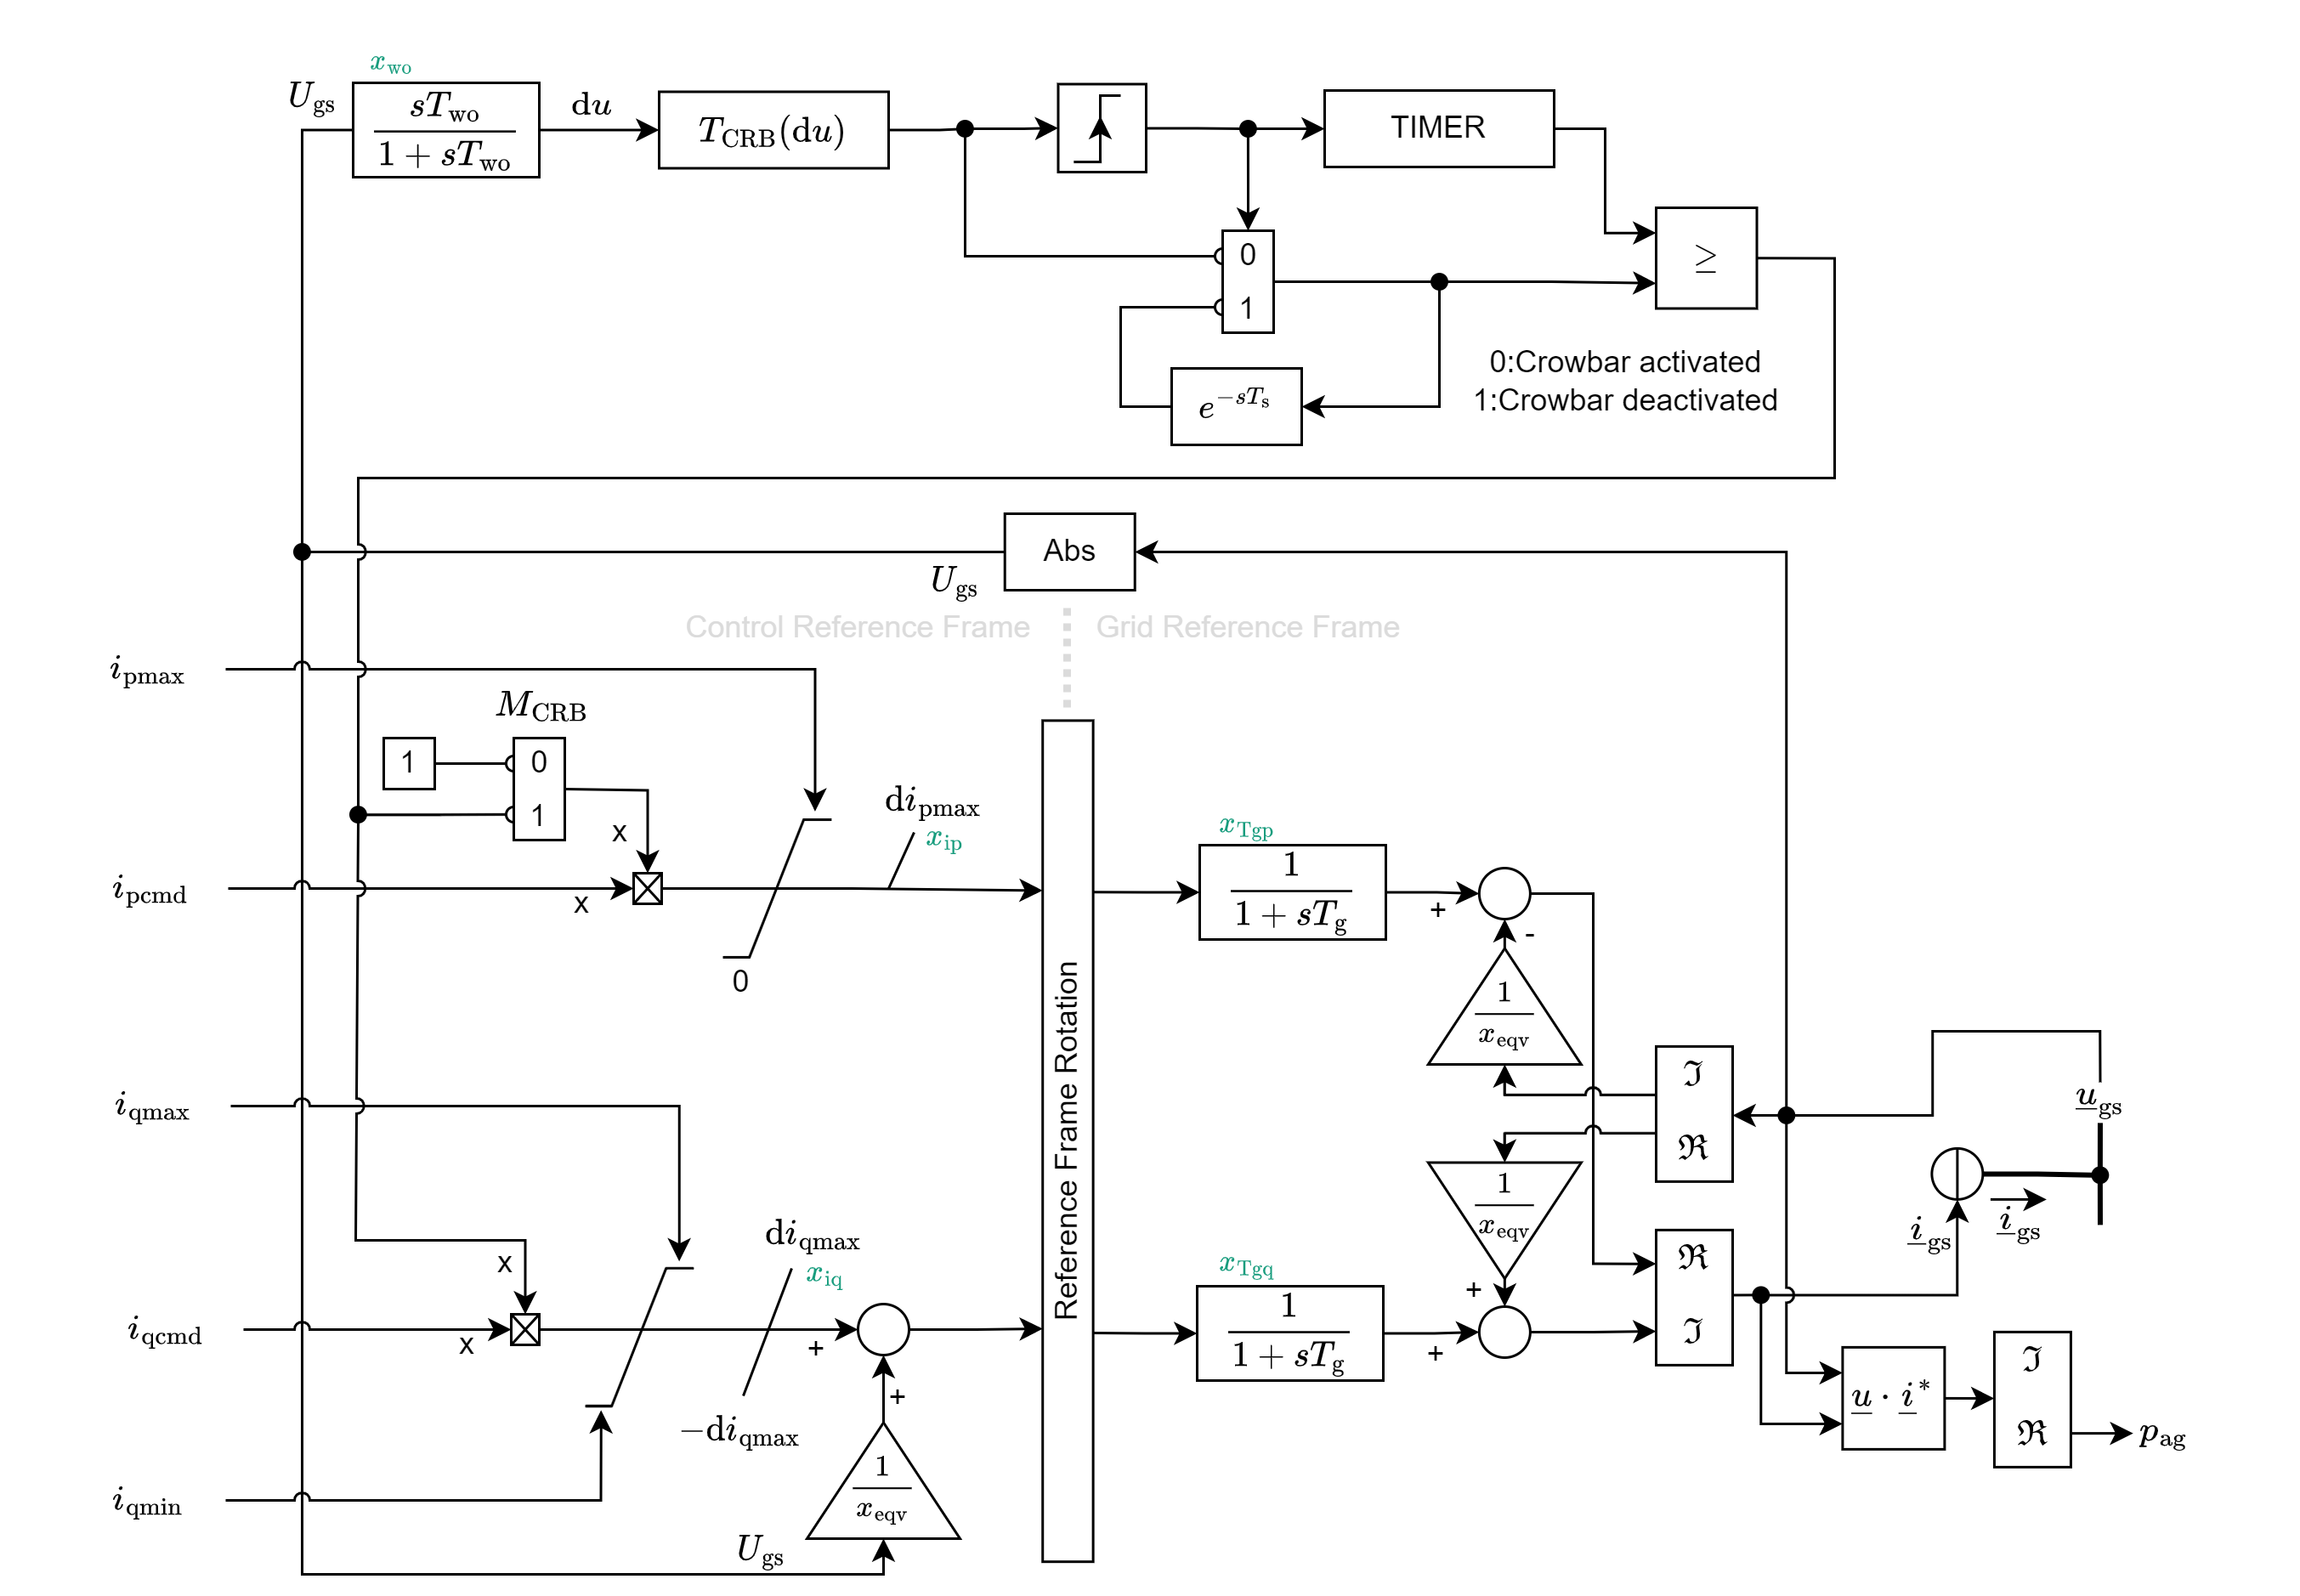
\includegraphics{drawings/WT_GS_3B.drawio.png}

}

\caption{\label{fig-generatorType3b}Wind turbine type 3B generator
system model, based on {[}1{]}}

\end{figure}%

The Type 3B Generator System models a DFIG with crowbar circuit.

In the model, as shown in Figure~\ref{fig-generatorType3b}, the crowbar
system is not physically modeled but instead represented by multiplying
the current commands by zero for a certain period of time when the
voltage module's derivative goes beyond a certain threshold {[}5{]}.

\begin{figure}

\begin{minipage}{0.50\linewidth}

\begin{figure}[H]

\centering{

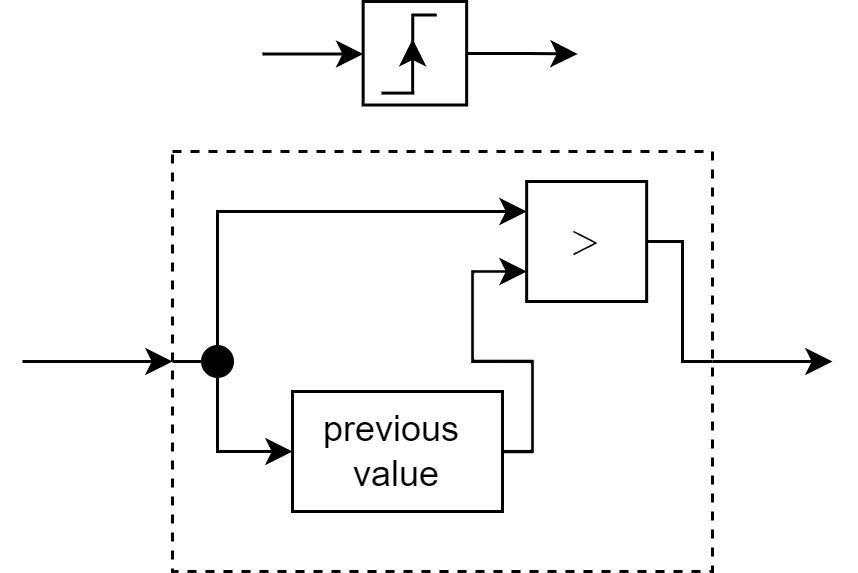
\includegraphics{drawings/WT_GS_3B_risingvalue.drawio.png}

}

\caption{\label{fig-generatorType3bRisingDetection}Rising value
detection, based on {[}1{]}}

\end{figure}%

\end{minipage}%
%
\begin{minipage}{0.50\linewidth}

\begin{figure}[H]

\centering{

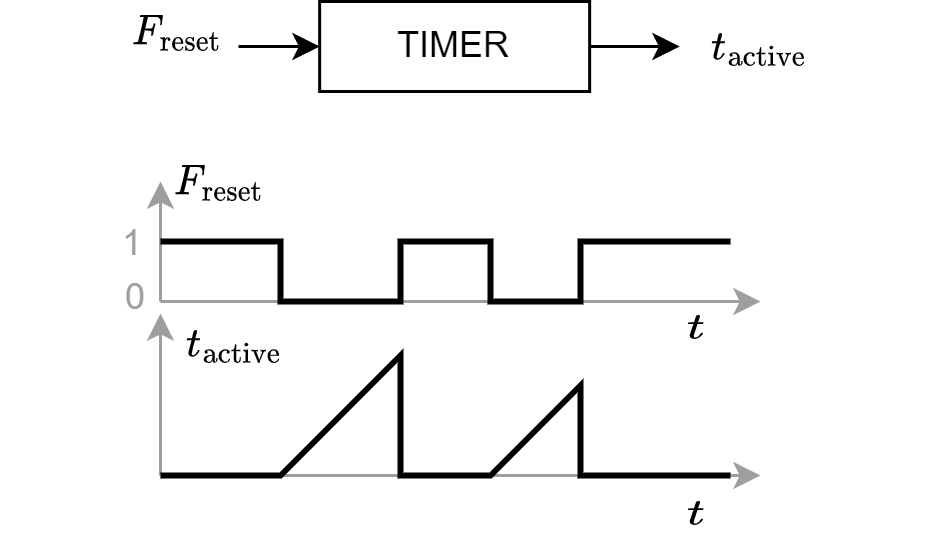
\includegraphics{drawings/WT_GS_3B_timer.drawio.png}

}

\caption{\label{fig-generatorType3bTimer}Timer, based on {[}1{]}}

\end{figure}%

\end{minipage}%

\end{figure}%

\subsubsection{Paramaters}\label{paramaters}

\paragraph{Type 3A}\label{type-3a-1}

\begin{longtable}[]{@{}
  >{\raggedright\arraybackslash}p{(\columnwidth - 12\tabcolsep) * \real{0.0600}}
  >{\raggedright\arraybackslash}p{(\columnwidth - 12\tabcolsep) * \real{0.0600}}
  >{\raggedright\arraybackslash}p{(\columnwidth - 12\tabcolsep) * \real{0.0500}}
  >{\raggedright\arraybackslash}p{(\columnwidth - 12\tabcolsep) * \real{0.2000}}
  >{\raggedright\arraybackslash}p{(\columnwidth - 12\tabcolsep) * \real{0.1000}}
  >{\raggedright\arraybackslash}p{(\columnwidth - 12\tabcolsep) * \real{0.4400}}
  >{\raggedright\arraybackslash}p{(\columnwidth - 12\tabcolsep) * \real{0.0700}}@{}}
\caption{Parameters of Type 3A Generator System, based on {[}1{]} and
\emph{DIgSILENT
PowerFactory}}\label{tbl-parametersGenSys3a}\tabularnewline
\toprule\noalign{}
\begin{minipage}[b]{\linewidth}\raggedright
name
\end{minipage} & \begin{minipage}[b]{\linewidth}\raggedright
type
\end{minipage} & \begin{minipage}[b]{\linewidth}\raggedright
unit
\end{minipage} & \begin{minipage}[b]{\linewidth}\raggedright
base
\end{minipage} & \begin{minipage}[b]{\linewidth}\raggedright
modelica name
\end{minipage} & \begin{minipage}[b]{\linewidth}\raggedright
description
\end{minipage} & \begin{minipage}[b]{\linewidth}\raggedright
typical value
\end{minipage} \\
\midrule\noalign{}
\endfirsthead
\toprule\noalign{}
\begin{minipage}[b]{\linewidth}\raggedright
name
\end{minipage} & \begin{minipage}[b]{\linewidth}\raggedright
type
\end{minipage} & \begin{minipage}[b]{\linewidth}\raggedright
unit
\end{minipage} & \begin{minipage}[b]{\linewidth}\raggedright
base
\end{minipage} & \begin{minipage}[b]{\linewidth}\raggedright
modelica name
\end{minipage} & \begin{minipage}[b]{\linewidth}\raggedright
description
\end{minipage} & \begin{minipage}[b]{\linewidth}\raggedright
typical value
\end{minipage} \\
\midrule\noalign{}
\endhead
\bottomrule\noalign{}
\endlastfoot
\(\mathrm{d}i_\mathrm{pmax}\) & float & pu/s & \(I_\mathrm{base}\) &
DIPMax & Active current ramp rate limit & 9999 \\
\(\mathrm{d}i_\mathrm{qmax}\) & float & pu/s & \(I_\mathrm{base}\) &
DIQMax & Reactive current ramp rate limit & 9999 \\
\(K_\mathrm{Pc}\) & float & - & - & KPc & Proportional gain of current
controller & 40 \\
\(T_\mathrm{Ic}\) & float & s & - & TIc & Integral gain of current
controller & 0.02 \\
\(x_\mathrm{eqv}\) & float & pu & \(Z_\mathrm{base}\) & XEqv & Transient
reactance (calculated from transient inductance like in {[}4{]}) &
0.4 \\
\end{longtable}

\paragraph{Type 3B}\label{type-3b-1}

\begin{longtable}[]{@{}
  >{\raggedright\arraybackslash}p{(\columnwidth - 12\tabcolsep) * \real{0.0600}}
  >{\raggedright\arraybackslash}p{(\columnwidth - 12\tabcolsep) * \real{0.0600}}
  >{\raggedright\arraybackslash}p{(\columnwidth - 12\tabcolsep) * \real{0.0500}}
  >{\raggedright\arraybackslash}p{(\columnwidth - 12\tabcolsep) * \real{0.2000}}
  >{\raggedright\arraybackslash}p{(\columnwidth - 12\tabcolsep) * \real{0.1000}}
  >{\raggedright\arraybackslash}p{(\columnwidth - 12\tabcolsep) * \real{0.4400}}
  >{\raggedright\arraybackslash}p{(\columnwidth - 12\tabcolsep) * \real{0.0700}}@{}}
\caption{Parameters of Type 3B Generator System, based on {[}1{]} and
\emph{DIgSILENT
PowerFactory}}\label{tbl-parametersGenSys3a}\tabularnewline
\toprule\noalign{}
\begin{minipage}[b]{\linewidth}\raggedright
name
\end{minipage} & \begin{minipage}[b]{\linewidth}\raggedright
type
\end{minipage} & \begin{minipage}[b]{\linewidth}\raggedright
unit
\end{minipage} & \begin{minipage}[b]{\linewidth}\raggedright
base
\end{minipage} & \begin{minipage}[b]{\linewidth}\raggedright
modelica name
\end{minipage} & \begin{minipage}[b]{\linewidth}\raggedright
description
\end{minipage} & \begin{minipage}[b]{\linewidth}\raggedright
typical value
\end{minipage} \\
\midrule\noalign{}
\endfirsthead
\toprule\noalign{}
\begin{minipage}[b]{\linewidth}\raggedright
name
\end{minipage} & \begin{minipage}[b]{\linewidth}\raggedright
type
\end{minipage} & \begin{minipage}[b]{\linewidth}\raggedright
unit
\end{minipage} & \begin{minipage}[b]{\linewidth}\raggedright
base
\end{minipage} & \begin{minipage}[b]{\linewidth}\raggedright
modelica name
\end{minipage} & \begin{minipage}[b]{\linewidth}\raggedright
description
\end{minipage} & \begin{minipage}[b]{\linewidth}\raggedright
typical value
\end{minipage} \\
\midrule\noalign{}
\endhead
\bottomrule\noalign{}
\endlastfoot
\(\mathrm{d}i_\mathrm{pmax}\) & float & pu/s & \(I_\mathrm{base}\) &
DIPMax & Active current ramp rate limit & 1 \\
\(\mathrm{d}i_\mathrm{qmax}\) & float & pu/s & \(I_\mathrm{base}\) &
DIQMax & Reactive current ramp rate limit & 100 \\
\(M_\mathrm{CRB}\) & boolean & - & - & KPc & Control mode & false \\
\(\mathbf{T_\mathrm{CRB}}\) & float & s & - & tCrb & look-up table:
Crowbar duration (output) as a function of voltage variation (input) &
{[}-99,0.1; -1,0.1; -0.1,0; 0,0{]} \\
\(T_\mathrm{g}\) & float & s & - & TG & Time constant of current
generation & 0.01 \\
\(T_\mathrm{wo}\) & float & s & - & TWo & Crowbar washout filter time
constant & 0.001 \\
\(x_\mathrm{eqv}\) & float & pu & \(Z_\mathrm{base}\) & XEqv & Transient
reactance (calculated from transient inductance like in {[}4{]}) & 10 \\
\end{longtable}

\subsubsection{Variables}\label{variables-7}

\paragraph{Inputs}\label{inputs-7}

\begin{longtable}[]{@{}
  >{\raggedright\arraybackslash}p{(\columnwidth - 10\tabcolsep) * \real{0.0600}}
  >{\raggedright\arraybackslash}p{(\columnwidth - 10\tabcolsep) * \real{0.0600}}
  >{\raggedright\arraybackslash}p{(\columnwidth - 10\tabcolsep) * \real{0.0500}}
  >{\raggedright\arraybackslash}p{(\columnwidth - 10\tabcolsep) * \real{0.2000}}
  >{\raggedright\arraybackslash}p{(\columnwidth - 10\tabcolsep) * \real{0.1000}}
  >{\raggedright\arraybackslash}p{(\columnwidth - 10\tabcolsep) * \real{0.4400}}@{}}
\caption{Inputs, based on {[}1{]} and
{[}5{]}}\label{tbl-inputsGensys}\tabularnewline
\toprule\noalign{}
\begin{minipage}[b]{\linewidth}\raggedright
name
\end{minipage} & \begin{minipage}[b]{\linewidth}\raggedright
type
\end{minipage} & \begin{minipage}[b]{\linewidth}\raggedright
unit
\end{minipage} & \begin{minipage}[b]{\linewidth}\raggedright
base
\end{minipage} & \begin{minipage}[b]{\linewidth}\raggedright
modelica name
\end{minipage} & \begin{minipage}[b]{\linewidth}\raggedright
description
\end{minipage} \\
\midrule\noalign{}
\endfirsthead
\toprule\noalign{}
\begin{minipage}[b]{\linewidth}\raggedright
name
\end{minipage} & \begin{minipage}[b]{\linewidth}\raggedright
type
\end{minipage} & \begin{minipage}[b]{\linewidth}\raggedright
unit
\end{minipage} & \begin{minipage}[b]{\linewidth}\raggedright
base
\end{minipage} & \begin{minipage}[b]{\linewidth}\raggedright
modelica name
\end{minipage} & \begin{minipage}[b]{\linewidth}\raggedright
description
\end{minipage} \\
\midrule\noalign{}
\endhead
\bottomrule\noalign{}
\endlastfoot
\(i_\mathrm{pcmd}\) & float & pu & \(I_\mathrm{base}\) & ipCmdPu &
Active current command \\
\(i_\mathrm{pmax}\) & float & pu & \(I_\mathrm{base}\) & ipMaxPu &
Maximum active current \\
\(i_\mathrm{qcmd}\) & float & pu & \(I_\mathrm{base}\) & iqCmdPu &
Reactive current command \\
\(i_\mathrm{qmax}\) & float & pu & \(I_\mathrm{base}\) & iqMaxPu &
Maximum reactive current \\
\(i_\mathrm{qmin}\) & float & pu & \(I_\mathrm{base}\) & iqMinPu &
Minimum reactive current \\
\(\underline{u}_\mathrm{gs}\) & complex & pu & \(U_\mathrm{base}\) &
terminal.V & Generator system terminal voltage \\
\end{longtable}

\paragraph{Outputs}\label{outputs-7}

\begin{longtable}[]{@{}
  >{\raggedright\arraybackslash}p{(\columnwidth - 10\tabcolsep) * \real{0.0600}}
  >{\raggedright\arraybackslash}p{(\columnwidth - 10\tabcolsep) * \real{0.0600}}
  >{\raggedright\arraybackslash}p{(\columnwidth - 10\tabcolsep) * \real{0.0500}}
  >{\raggedright\arraybackslash}p{(\columnwidth - 10\tabcolsep) * \real{0.2000}}
  >{\raggedright\arraybackslash}p{(\columnwidth - 10\tabcolsep) * \real{0.1000}}
  >{\raggedright\arraybackslash}p{(\columnwidth - 10\tabcolsep) * \real{0.4400}}@{}}
\caption{Outputs, based on
{[}1{]}}\label{tbl-outputsGensys}\tabularnewline
\toprule\noalign{}
\begin{minipage}[b]{\linewidth}\raggedright
name
\end{minipage} & \begin{minipage}[b]{\linewidth}\raggedright
type
\end{minipage} & \begin{minipage}[b]{\linewidth}\raggedright
unit
\end{minipage} & \begin{minipage}[b]{\linewidth}\raggedright
base
\end{minipage} & \begin{minipage}[b]{\linewidth}\raggedright
modelica name
\end{minipage} & \begin{minipage}[b]{\linewidth}\raggedright
description
\end{minipage} \\
\midrule\noalign{}
\endfirsthead
\toprule\noalign{}
\begin{minipage}[b]{\linewidth}\raggedright
name
\end{minipage} & \begin{minipage}[b]{\linewidth}\raggedright
type
\end{minipage} & \begin{minipage}[b]{\linewidth}\raggedright
unit
\end{minipage} & \begin{minipage}[b]{\linewidth}\raggedright
base
\end{minipage} & \begin{minipage}[b]{\linewidth}\raggedright
modelica name
\end{minipage} & \begin{minipage}[b]{\linewidth}\raggedright
description
\end{minipage} \\
\midrule\noalign{}
\endhead
\bottomrule\noalign{}
\endlastfoot
\(p_\mathrm{ag}\) & float & pu & \(S_\mathrm{base}\) & PAgPu & Air gap
power (before losses due to connection impedance and admittance) \\
\(\underline{i}_\mathrm{gs}\) & complex & pu & \(I_\mathrm{base}\) &
terminal.i & Generator system terminal current \\
\end{longtable}

\subsubsection{Initial equations}\label{initial-equations-4}

For the used initialization helper variables, see
Section~\ref{sec-initHelpersGlobal}.

\begin{equation}\phantomsection\label{eq-initXip}{ 
x_\mathrm{Ip} = P_\mathrm{ord\,0}/U_0
}\end{equation}

\begin{equation}\phantomsection\label{eq-initXiq}{ 
x_\mathrm{Iq} = Q_\mathrm{ord\,0}/U_0
}\end{equation}

\begin{equation}\phantomsection\label{eq-initXpip}{ 
x_\mathrm{PIp} = x_\mathrm{PIq} = 0
}\end{equation}

\begin{equation}\phantomsection\label{eq-initXintp}{ 
x_\mathrm{intp} = I_\mathrm{gs\,re\,0} + \frac{U_\mathrm{gs\,im\,0}}{X_\mathrm{eqv}}
}\end{equation}

\begin{equation}\phantomsection\label{eq-initXintq}{ 
x_\mathrm{intq} = I_\mathrm{gs\,im\,0} - \frac{U_\mathrm{gs\,re\,0}}{X_\mathrm{eqv}}
}\end{equation}

\begin{equation}\phantomsection\label{eq-initXtgp}{ 
x_\mathrm{Tgp} = I_\mathrm{gs\,re\,0} + \frac{U_\mathrm{gs\,im\,0}}{X_\mathrm{eqv}}
}\end{equation}

\begin{equation}\phantomsection\label{eq-initXtgq}{ 
x_\mathrm{Tgq} = I_\mathrm{gs\,im\,0} - \frac{U_\mathrm{gs\,re\,0}}{X_\mathrm{eqv}}
}\end{equation}

\begin{equation}\phantomsection\label{eq-initXwo}{ 
x_\mathrm{wo} = 0
}\end{equation}

\subsubsection{Assumptions in Modelica
implementation}\label{assumptions-in-modelica-implementation}

\subsection{Grid measurement module}\label{grid-measurement-module}

Calculates measured values from complex grid voltage and current and
grid frequency.

\begin{figure}

\centering{

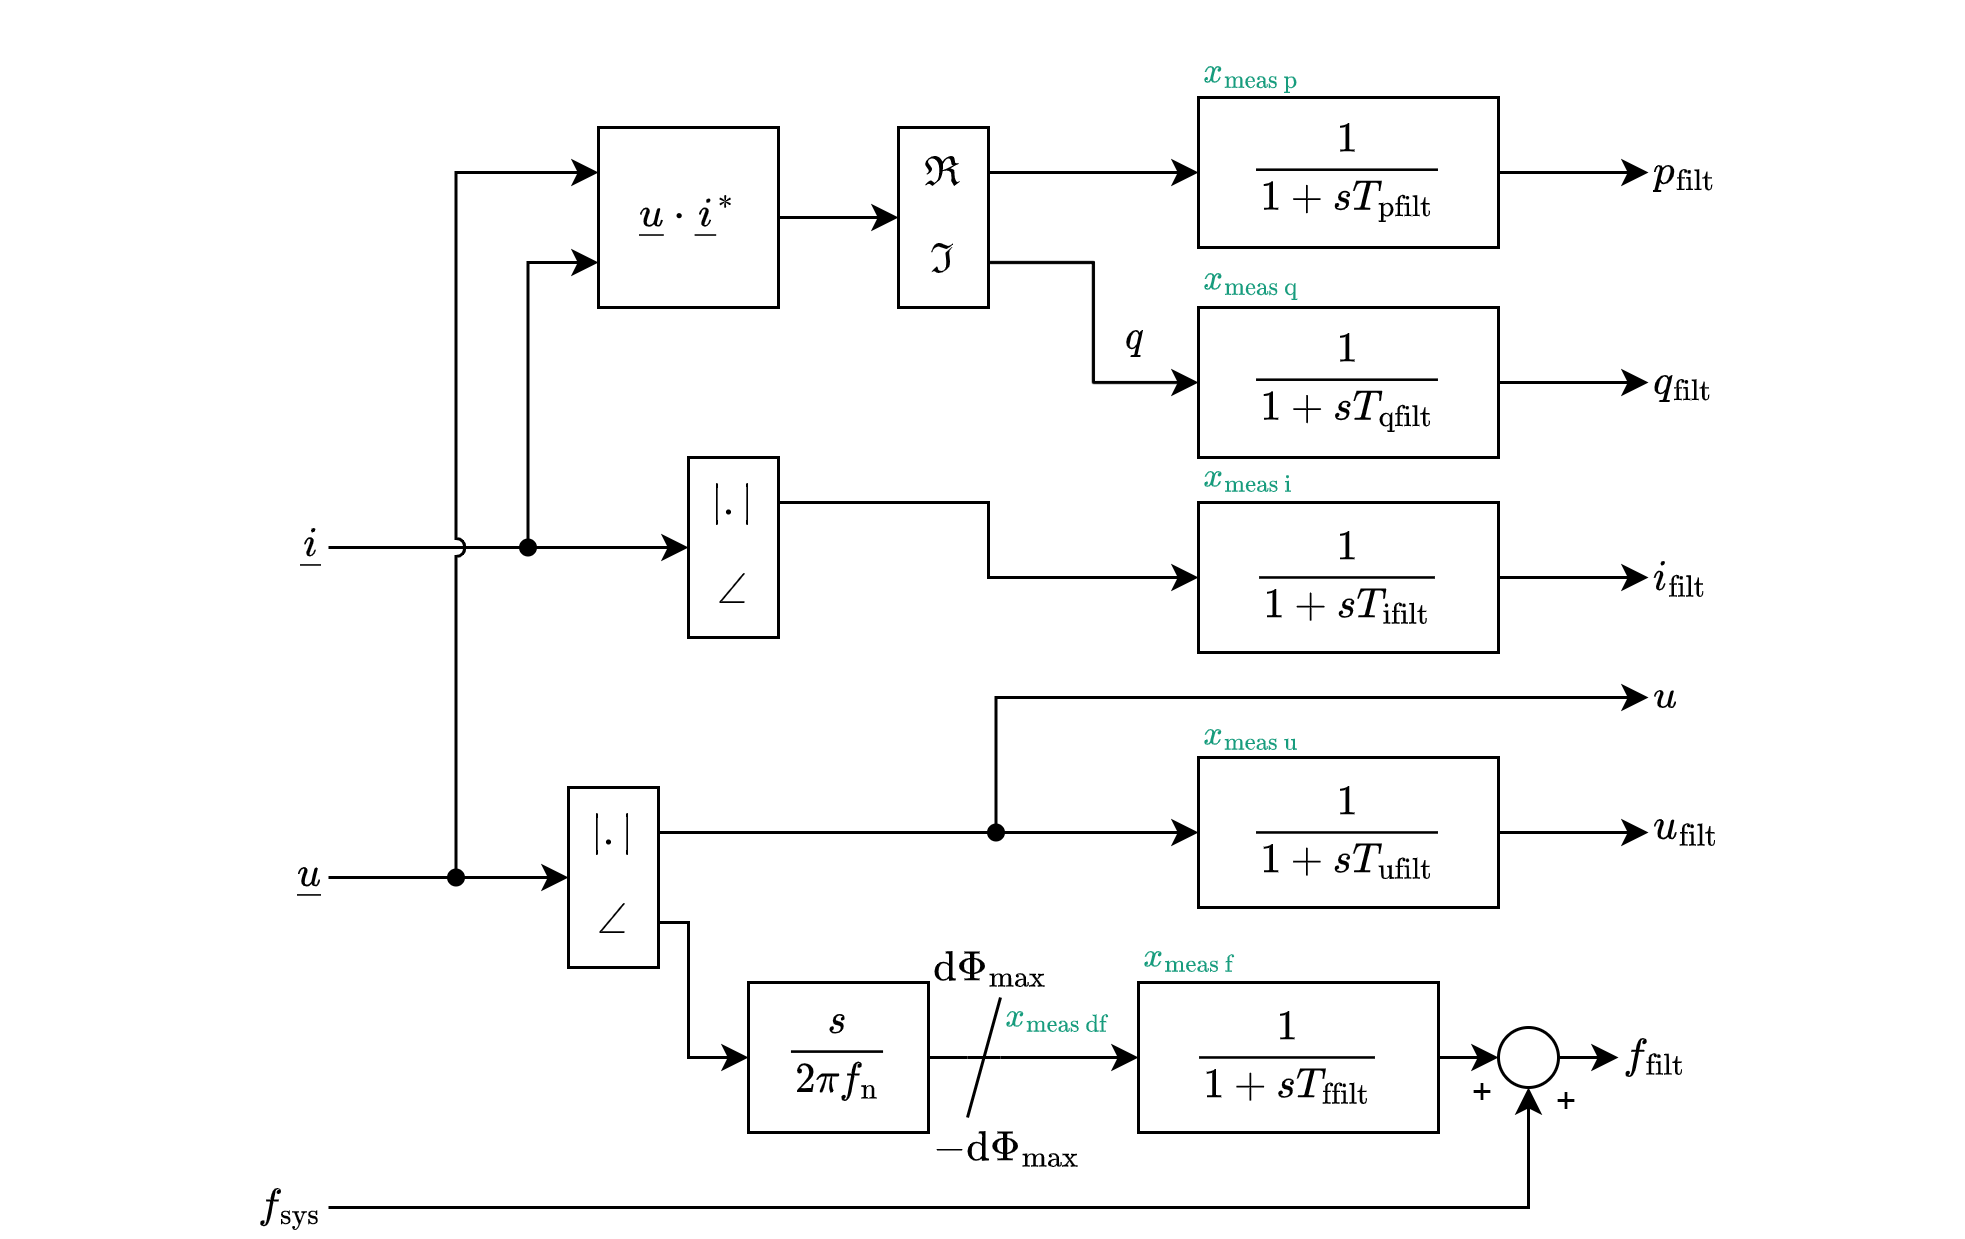
\includegraphics{drawings/IEC_WT_meas.drawio.png}

}

\caption{\label{fig-measurementModule}Grid measurement module}

\end{figure}%

\subsubsection{Parameters}\label{parameters-6}

\begin{longtable}[]{@{}
  >{\raggedright\arraybackslash}p{(\columnwidth - 10\tabcolsep) * \real{0.0600}}
  >{\raggedright\arraybackslash}p{(\columnwidth - 10\tabcolsep) * \real{0.0600}}
  >{\raggedright\arraybackslash}p{(\columnwidth - 10\tabcolsep) * \real{0.0500}}
  >{\raggedright\arraybackslash}p{(\columnwidth - 10\tabcolsep) * \real{0.2000}}
  >{\raggedright\arraybackslash}p{(\columnwidth - 10\tabcolsep) * \real{0.4400}}
  >{\raggedright\arraybackslash}p{(\columnwidth - 10\tabcolsep) * \real{0.0700}}@{}}
\caption{Parameters of measurement module, based on {[}1{]} and
\emph{DIgSILENT
PowerFactory}}\label{tbl-parametersMeasurement}\tabularnewline
\toprule\noalign{}
\begin{minipage}[b]{\linewidth}\raggedright
name
\end{minipage} & \begin{minipage}[b]{\linewidth}\raggedright
type
\end{minipage} & \begin{minipage}[b]{\linewidth}\raggedright
unit
\end{minipage} & \begin{minipage}[b]{\linewidth}\raggedright
base
\end{minipage} & \begin{minipage}[b]{\linewidth}\raggedright
description
\end{minipage} & \begin{minipage}[b]{\linewidth}\raggedright
typical value
\end{minipage} \\
\midrule\noalign{}
\endfirsthead
\toprule\noalign{}
\begin{minipage}[b]{\linewidth}\raggedright
name
\end{minipage} & \begin{minipage}[b]{\linewidth}\raggedright
type
\end{minipage} & \begin{minipage}[b]{\linewidth}\raggedright
unit
\end{minipage} & \begin{minipage}[b]{\linewidth}\raggedright
base
\end{minipage} & \begin{minipage}[b]{\linewidth}\raggedright
description
\end{minipage} & \begin{minipage}[b]{\linewidth}\raggedright
typical value
\end{minipage} \\
\midrule\noalign{}
\endhead
\bottomrule\noalign{}
\endlastfoot
\(\mathrm{d}\Phi_\mathrm{max}\) & float & pu &
\(f_\mathrm{n}/\mathrm{s}\) & Max. rate of change of frequency, should
be larger than any ROCOF protection threshold in the system. & 0.1 (5
Hz/s) \\
\(T_\mathrm{ffilt}\) & float & s & - & frequency measurement fitler time
constant & 0.005 \\
\(T_\mathrm{ifilt}\) & float & s & - & current measurement fitler time
constant & 0.005 \\
\(T_\mathrm{pfilt}\) & float & s & - & active power measurement fitler
time constant & 0.005 \\
\(T_\mathrm{qfilt}\) & float & s & - & reactive power measurement fitler
time constant & 0.005 \\
\(T_\mathrm{ufilt}\) & float & s & - & voltage measurement fitler time
constant & 0.005 \\
& & & & & \\
\end{longtable}

\subsubsection{Variables}\label{variables-8}

\paragraph{Inputs}\label{inputs-8}

\begin{longtable}[]{@{}
  >{\raggedright\arraybackslash}p{(\columnwidth - 8\tabcolsep) * \real{0.1860}}
  >{\raggedright\arraybackslash}p{(\columnwidth - 8\tabcolsep) * \real{0.0814}}
  >{\raggedright\arraybackslash}p{(\columnwidth - 8\tabcolsep) * \real{0.0465}}
  >{\raggedright\arraybackslash}p{(\columnwidth - 8\tabcolsep) * \real{0.2558}}
  >{\raggedright\arraybackslash}p{(\columnwidth - 8\tabcolsep) * \real{0.4302}}@{}}
\caption{Inputs, based on
{[}1{]}}\label{tbl-inputsMeasurement}\tabularnewline
\toprule\noalign{}
\begin{minipage}[b]{\linewidth}\raggedright
name
\end{minipage} & \begin{minipage}[b]{\linewidth}\raggedright
type
\end{minipage} & \begin{minipage}[b]{\linewidth}\raggedright
unit
\end{minipage} & \begin{minipage}[b]{\linewidth}\raggedright
base
\end{minipage} & \begin{minipage}[b]{\linewidth}\raggedright
description
\end{minipage} \\
\midrule\noalign{}
\endfirsthead
\toprule\noalign{}
\begin{minipage}[b]{\linewidth}\raggedright
name
\end{minipage} & \begin{minipage}[b]{\linewidth}\raggedright
type
\end{minipage} & \begin{minipage}[b]{\linewidth}\raggedright
unit
\end{minipage} & \begin{minipage}[b]{\linewidth}\raggedright
base
\end{minipage} & \begin{minipage}[b]{\linewidth}\raggedright
description
\end{minipage} \\
\midrule\noalign{}
\endhead
\bottomrule\noalign{}
\endlastfoot
\(f_\mathrm{sys}\) & float & pu & \(\Omega_\mathrm{base}\) & grid
frequency of global power system \\
\(\underline{i}\) & complex & pu & \(I_\mathrm{base}\) & measured
current \\
\(\underline{u}\) & complex & pu & \(U_\mathrm{base}\) & measured
voltage \\
\end{longtable}

\paragraph{Outputs}\label{outputs-8}

\begin{longtable}[]{@{}
  >{\raggedright\arraybackslash}p{(\columnwidth - 8\tabcolsep) * \real{0.2125}}
  >{\raggedright\arraybackslash}p{(\columnwidth - 8\tabcolsep) * \real{0.0625}}
  >{\raggedright\arraybackslash}p{(\columnwidth - 8\tabcolsep) * \real{0.0500}}
  >{\raggedright\arraybackslash}p{(\columnwidth - 8\tabcolsep) * \real{0.2125}}
  >{\raggedright\arraybackslash}p{(\columnwidth - 8\tabcolsep) * \real{0.4625}}@{}}
\caption{Outputs, based on
{[}1{]}}\label{tbl-outputsMeasurement}\tabularnewline
\toprule\noalign{}
\begin{minipage}[b]{\linewidth}\raggedright
name
\end{minipage} & \begin{minipage}[b]{\linewidth}\raggedright
type
\end{minipage} & \begin{minipage}[b]{\linewidth}\raggedright
unit
\end{minipage} & \begin{minipage}[b]{\linewidth}\raggedright
base
\end{minipage} & \begin{minipage}[b]{\linewidth}\raggedright
description
\end{minipage} \\
\midrule\noalign{}
\endfirsthead
\toprule\noalign{}
\begin{minipage}[b]{\linewidth}\raggedright
name
\end{minipage} & \begin{minipage}[b]{\linewidth}\raggedright
type
\end{minipage} & \begin{minipage}[b]{\linewidth}\raggedright
unit
\end{minipage} & \begin{minipage}[b]{\linewidth}\raggedright
base
\end{minipage} & \begin{minipage}[b]{\linewidth}\raggedright
description
\end{minipage} \\
\midrule\noalign{}
\endhead
\bottomrule\noalign{}
\endlastfoot
\(f_\mathrm{filt}\) & float & pu & \(\Omega_\mathrm{base}\) & frequency
with measurement delay \\
\(i_\mathrm{filt}\) & float & pu & \(I_\mathrm{base}\) & current with
measurement delay \\
\(p_\mathrm{filt}\) & float & pu & \(S_\mathrm{base}\) & active power
with measurement delay \\
\(q_\mathrm{filt}\) & float & pu & \(S_\mathrm{base}\) & reactive power
with measurement delay \\
\(u\) & float & pu & \(U_\mathrm{base}\) & voltage without measurement
delay \\
\(u_\mathrm{filt}\) & float & pu & \(U_\mathrm{base}\) & voltage with
measurement delay \\
\end{longtable}

\subsubsection{Initial equations}\label{initial-equations-5}

For the used initialization helper variables, see
Section~\ref{sec-initHelpersGlobal}.

\begin{equation}\phantomsection\label{eq-initXmeasp}{
x_\mathrm{meas\,p} = P_0
}\end{equation}

\begin{equation}\phantomsection\label{eq-initXmeasq}{
x_\mathrm{meas\,q} = Q_0
}\end{equation}

\begin{equation}\phantomsection\label{eq-initXmeasi}{
x_\mathrm{meas\,i} = \frac{\sqrt{P_0^2 + Q_0^2}}{U_0}
}\end{equation}

\begin{equation}\phantomsection\label{eq-initXmeasu}{
x_\mathrm{meas\,u} = U_0
}\end{equation}

\begin{equation}\phantomsection\label{eq-initXmeasf}{
x_\mathrm{meas\,f} = x_\mathrm{meas\,df} = 0
}\end{equation}

\subsection{Protection module}\label{protection-module}

The grid protection module offers protection against both over-voltage
and under-voltage, as well as over-frequency and under-frequency
conditions. As desribed in {[}1{]}, this time-based grid protection has
specific ranges of protection levels along with associated disconnection
times.

\begin{figure}[H]

{\centering 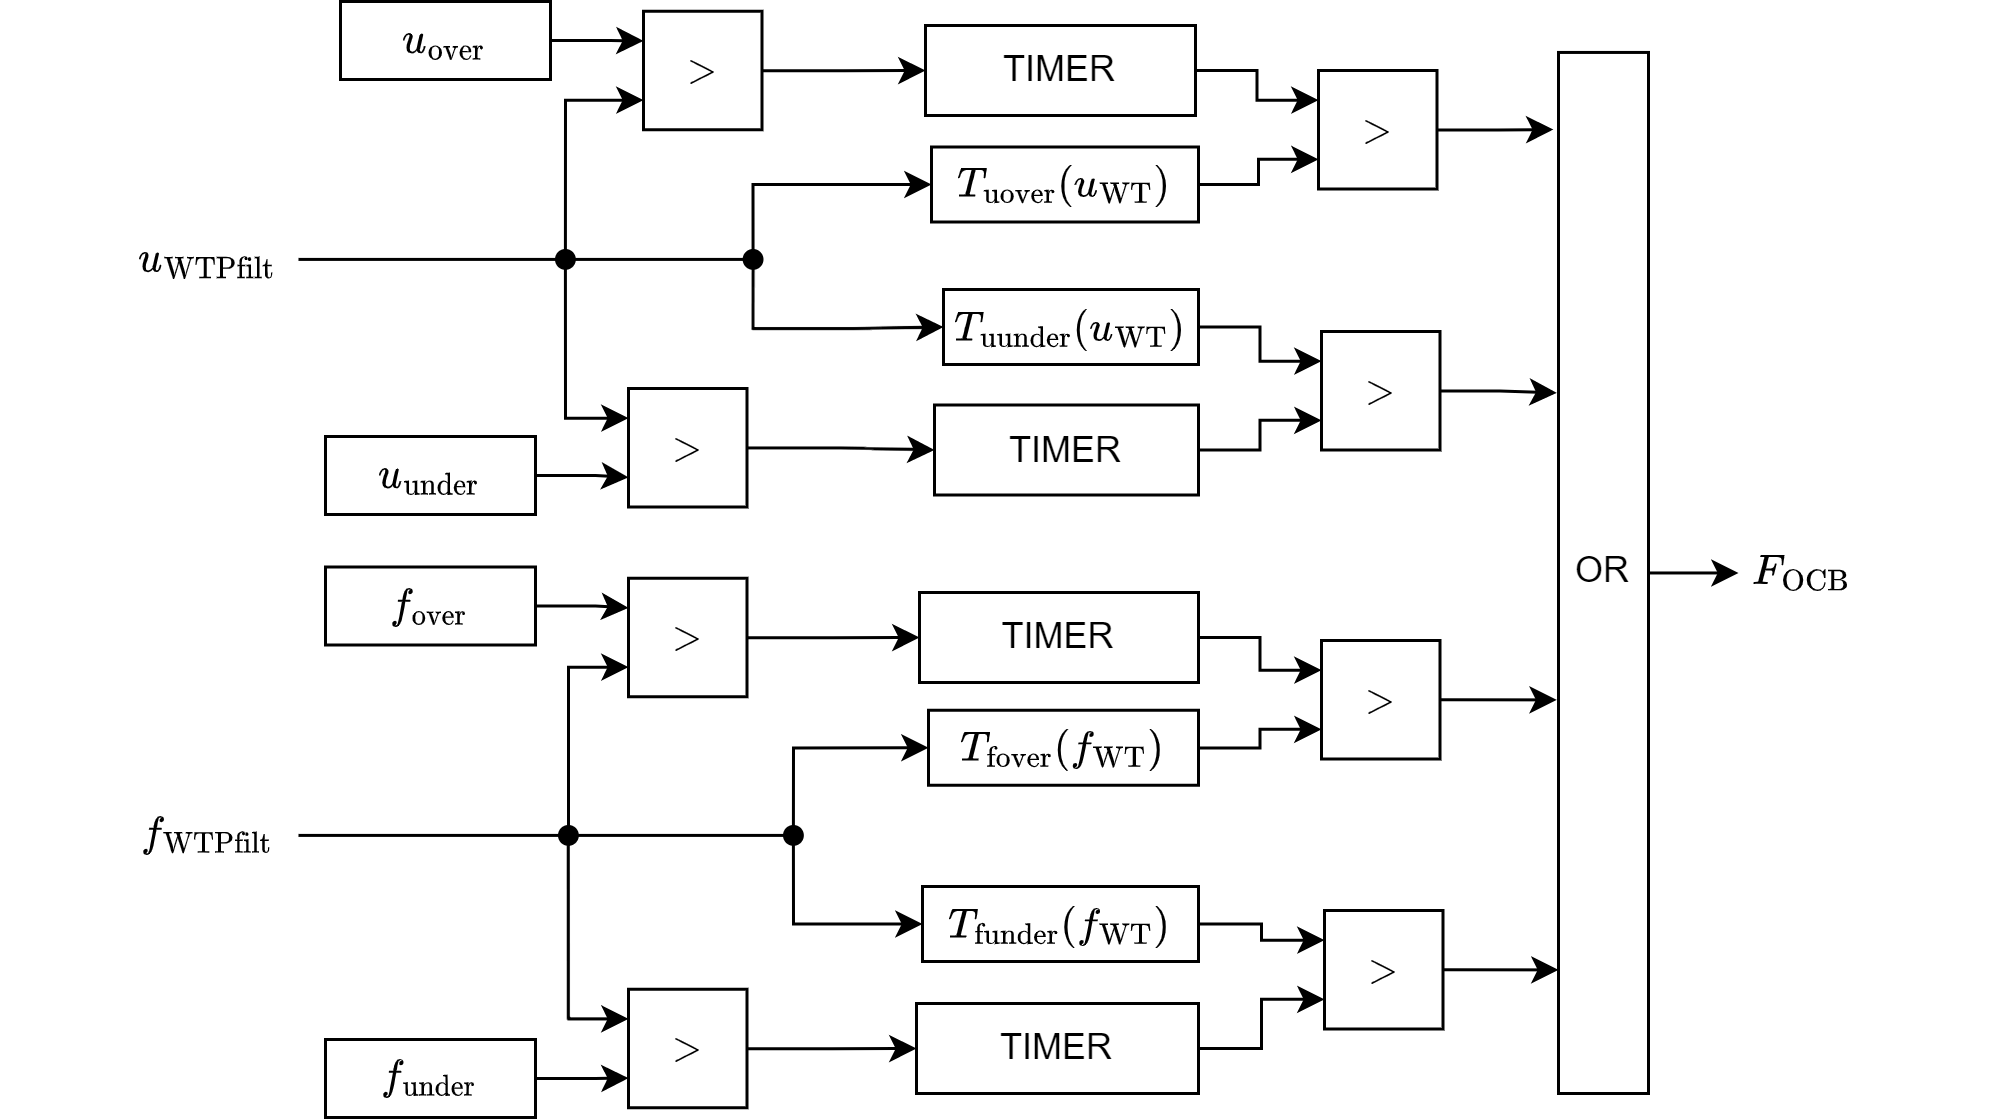
\includegraphics{drawings/Grid_Protection.drawio.png}

}

\caption{Grid protecton system module (timer: see
Figure~\ref{fig-generatorType3bTimer})}

\end{figure}%

\subsubsection{Parameters}\label{parameters-7}

\begin{longtable}[]{@{}
  >{\raggedright\arraybackslash}p{(\columnwidth - 10\tabcolsep) * \real{0.0600}}
  >{\raggedright\arraybackslash}p{(\columnwidth - 10\tabcolsep) * \real{0.0600}}
  >{\raggedright\arraybackslash}p{(\columnwidth - 10\tabcolsep) * \real{0.0500}}
  >{\raggedright\arraybackslash}p{(\columnwidth - 10\tabcolsep) * \real{0.2000}}
  >{\raggedright\arraybackslash}p{(\columnwidth - 10\tabcolsep) * \real{0.4400}}
  >{\raggedright\arraybackslash}p{(\columnwidth - 10\tabcolsep) * \real{0.0700}}@{}}
\caption{Parameters of measurement module, based on {[}1{]} and
\emph{DIgSILENT
PowerFactory}}\label{tbl-parametersProtection}\tabularnewline
\toprule\noalign{}
\begin{minipage}[b]{\linewidth}\raggedright
name
\end{minipage} & \begin{minipage}[b]{\linewidth}\raggedright
type
\end{minipage} & \begin{minipage}[b]{\linewidth}\raggedright
unit
\end{minipage} & \begin{minipage}[b]{\linewidth}\raggedright
base
\end{minipage} & \begin{minipage}[b]{\linewidth}\raggedright
description
\end{minipage} & \begin{minipage}[b]{\linewidth}\raggedright
typical value
\end{minipage} \\
\midrule\noalign{}
\endfirsthead
\toprule\noalign{}
\begin{minipage}[b]{\linewidth}\raggedright
name
\end{minipage} & \begin{minipage}[b]{\linewidth}\raggedright
type
\end{minipage} & \begin{minipage}[b]{\linewidth}\raggedright
unit
\end{minipage} & \begin{minipage}[b]{\linewidth}\raggedright
base
\end{minipage} & \begin{minipage}[b]{\linewidth}\raggedright
description
\end{minipage} & \begin{minipage}[b]{\linewidth}\raggedright
typical value
\end{minipage} \\
\midrule\noalign{}
\endhead
\bottomrule\noalign{}
\endlastfoot
\(f_\mathrm{over}\) & float & pu & \(f_\mathrm{n}\) & over frequency
protection threshold of WT & 1.02 \\
\(f_\mathrm{under}\) & float & pu & \(f_\mathrm{n}\) & under frequency
protection threshold of WT & 0.98 \\
\(\mathbf{T_\mathrm{fover}}(f_\mathrm{WT})\) & float & s & - &
lookup-table: disconnection time as a function of over frequency &
{[}1.02,1800; 1.03,1800; 1.03,0.1{]} \\
\(\mathbf{T_\mathrm{funder}}(f_\mathrm{WT})\) & float & s & - &
lookup-table: disconnection time as a function of under frequency &
{[}0.95,0.1; 0.95,1800; 0.98,1800{]} \\
\(\mathbf{T_\mathrm{uover}}(u_\mathrm{WT})\) & float & s & - &
lookup-table: disconnection time as a function of over voltage &
{[}1.2,60; 1.2,0.1; 1.3,0.1{]} \\
\(\mathbf{T_\mathrm{uunder}}(u_\mathrm{WT})\) & float & s & - &
lookup-table: disconnection time as a function of under voltage &
{[}0,0.15; 0.85,3{]} \\
\(u_\mathrm{over}\) & float & pu & \(U_\mathrm{base}\) & over voltage
protection threshold of WT & 1.2 \\
\(u_\mathrm{under}\) & float & pu & \(U_\mathrm{base}\) & under voltage
protection threshold of WT & 0.85 \\
\end{longtable}

\subsubsection{Variables}\label{variables-9}

\paragraph{Inputs}\label{inputs-9}

\begin{longtable}[]{@{}
  >{\raggedright\arraybackslash}p{(\columnwidth - 8\tabcolsep) * \real{0.2410}}
  >{\raggedright\arraybackslash}p{(\columnwidth - 8\tabcolsep) * \real{0.0602}}
  >{\raggedright\arraybackslash}p{(\columnwidth - 8\tabcolsep) * \real{0.0482}}
  >{\raggedright\arraybackslash}p{(\columnwidth - 8\tabcolsep) * \real{0.2651}}
  >{\raggedright\arraybackslash}p{(\columnwidth - 8\tabcolsep) * \real{0.3855}}@{}}
\caption{Inputs, based on
{[}1{]}}\label{tbl-inputsProtection}\tabularnewline
\toprule\noalign{}
\begin{minipage}[b]{\linewidth}\raggedright
name
\end{minipage} & \begin{minipage}[b]{\linewidth}\raggedright
type
\end{minipage} & \begin{minipage}[b]{\linewidth}\raggedright
unit
\end{minipage} & \begin{minipage}[b]{\linewidth}\raggedright
base
\end{minipage} & \begin{minipage}[b]{\linewidth}\raggedright
description
\end{minipage} \\
\midrule\noalign{}
\endfirsthead
\toprule\noalign{}
\begin{minipage}[b]{\linewidth}\raggedright
name
\end{minipage} & \begin{minipage}[b]{\linewidth}\raggedright
type
\end{minipage} & \begin{minipage}[b]{\linewidth}\raggedright
unit
\end{minipage} & \begin{minipage}[b]{\linewidth}\raggedright
base
\end{minipage} & \begin{minipage}[b]{\linewidth}\raggedright
description
\end{minipage} \\
\midrule\noalign{}
\endhead
\bottomrule\noalign{}
\endlastfoot
\(f_\mathrm{WTPfilt}\) & float & pu & \(\Omega_\mathrm{base}\) &
Measured frequency of wind plant \\
\(u_\mathrm{WTPfilt}\) & float & pu & \(U_\mathrm{base}\) & Measured
voltage of wind plant \\
\end{longtable}

\paragraph{Outputs}\label{outputs-9}

\begin{longtable}[]{@{}
  >{\raggedright\arraybackslash}p{(\columnwidth - 8\tabcolsep) * \real{0.2424}}
  >{\raggedright\arraybackslash}p{(\columnwidth - 8\tabcolsep) * \real{0.1061}}
  >{\raggedright\arraybackslash}p{(\columnwidth - 8\tabcolsep) * \real{0.0606}}
  >{\raggedright\arraybackslash}p{(\columnwidth - 8\tabcolsep) * \real{0.0606}}
  >{\raggedright\arraybackslash}p{(\columnwidth - 8\tabcolsep) * \real{0.5303}}@{}}
\caption{Outputs, based on
{[}1{]}}\label{tbl-outputsProtection}\tabularnewline
\toprule\noalign{}
\begin{minipage}[b]{\linewidth}\raggedright
name
\end{minipage} & \begin{minipage}[b]{\linewidth}\raggedright
type
\end{minipage} & \begin{minipage}[b]{\linewidth}\raggedright
unit
\end{minipage} & \begin{minipage}[b]{\linewidth}\raggedright
base
\end{minipage} & \begin{minipage}[b]{\linewidth}\raggedright
description
\end{minipage} \\
\midrule\noalign{}
\endfirsthead
\toprule\noalign{}
\begin{minipage}[b]{\linewidth}\raggedright
name
\end{minipage} & \begin{minipage}[b]{\linewidth}\raggedright
type
\end{minipage} & \begin{minipage}[b]{\linewidth}\raggedright
unit
\end{minipage} & \begin{minipage}[b]{\linewidth}\raggedright
base
\end{minipage} & \begin{minipage}[b]{\linewidth}\raggedright
description
\end{minipage} \\
\midrule\noalign{}
\endhead
\bottomrule\noalign{}
\endlastfoot
\(F_\mathrm{OCB}\) & boolean & - & - & Flag-signal to open circuit
breaker \\
\end{longtable}

\section{Wind power plant model}\label{wind-power-plant-model}

\begin{figure}

\centering{

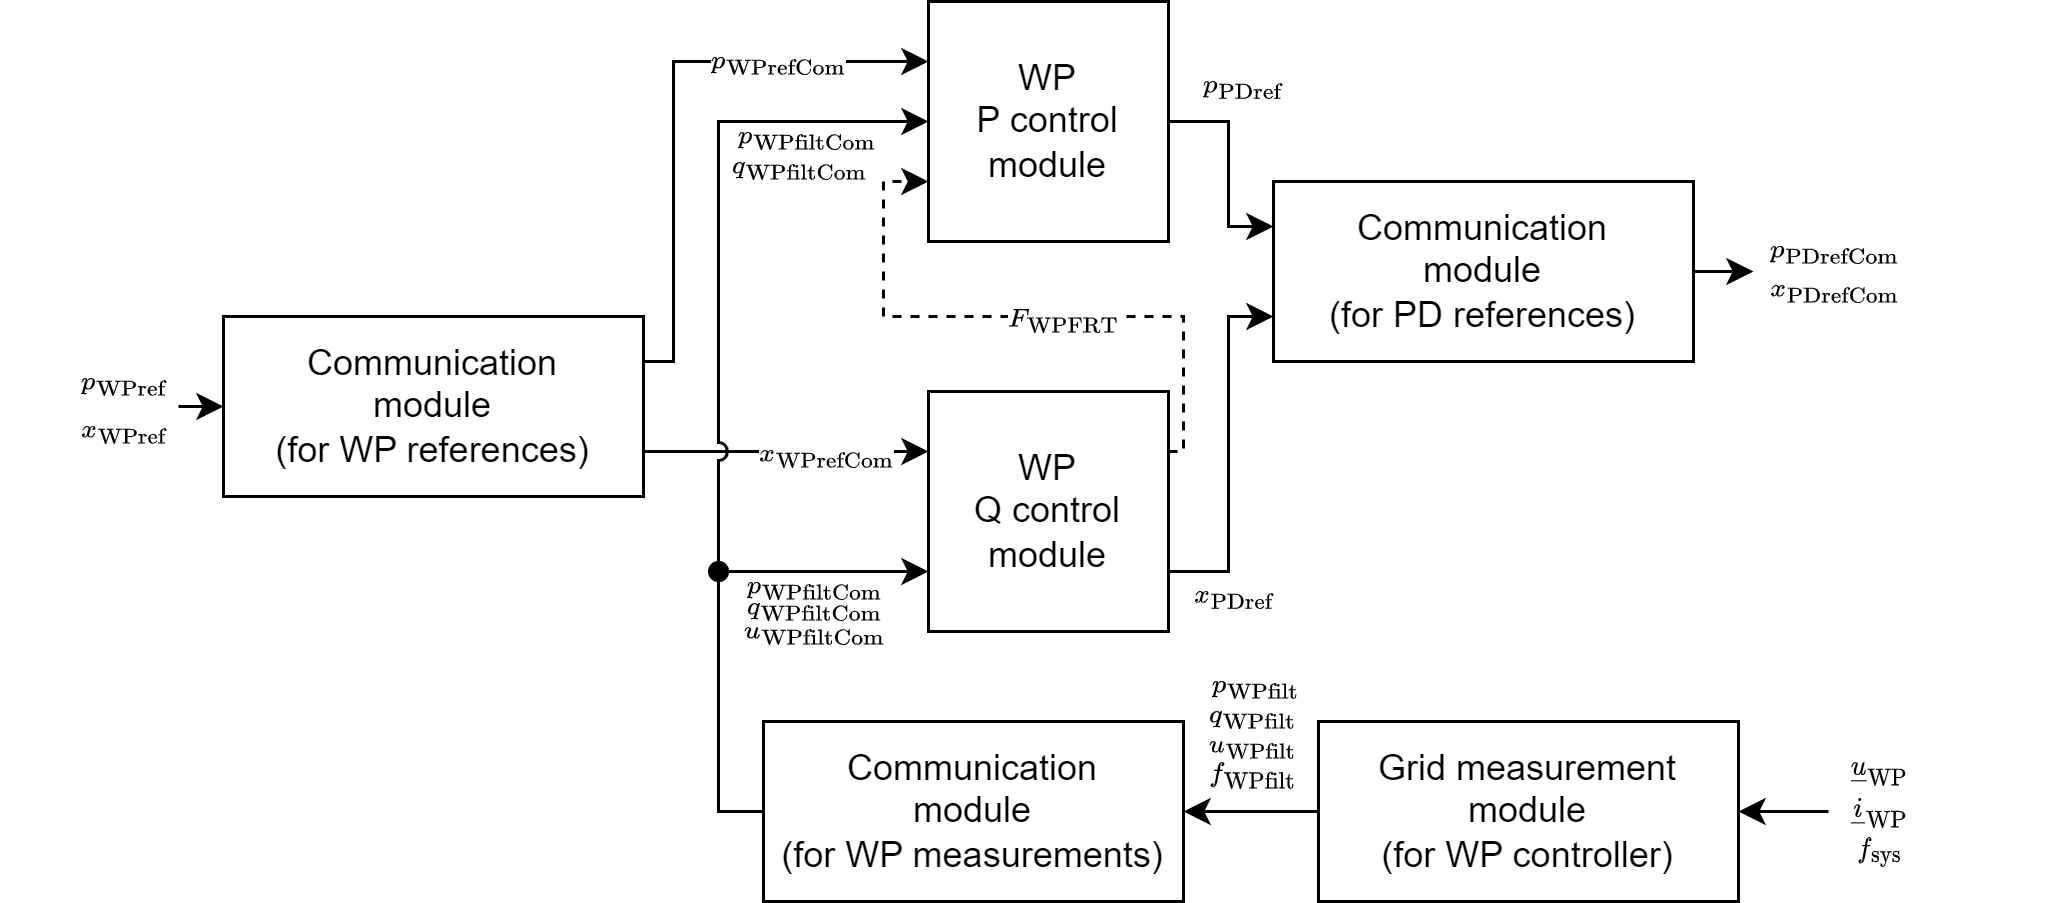
\includegraphics{drawings/WP_control_and_communication.drawio.png}

}

\caption{\label{fig-wp}Wind plant control and communictaion, based on
{[}1{]}}

\end{figure}%

The Wind Plant (WP) model includes two controllers: active power /
frequency controller (Figure~\ref{fig-wpActivePower}) and and reactive
power / voltage control (Figure~\ref{fig-wpReactivePower}).

Both, the P and Q controllers, freeze their state variables during FRT.

The WP model controls one single Point of Common Coupling (PCC).
According to {[}1{]} it is normally enough to use a single aggregated
model for all WTs in a WP. Still, also large WP can be modeled by using
multiple WP models which all get the same reference values from the WP
controller.

\subsection{WP P Control}\label{wp-p-control}

\begin{figure}

\centering{

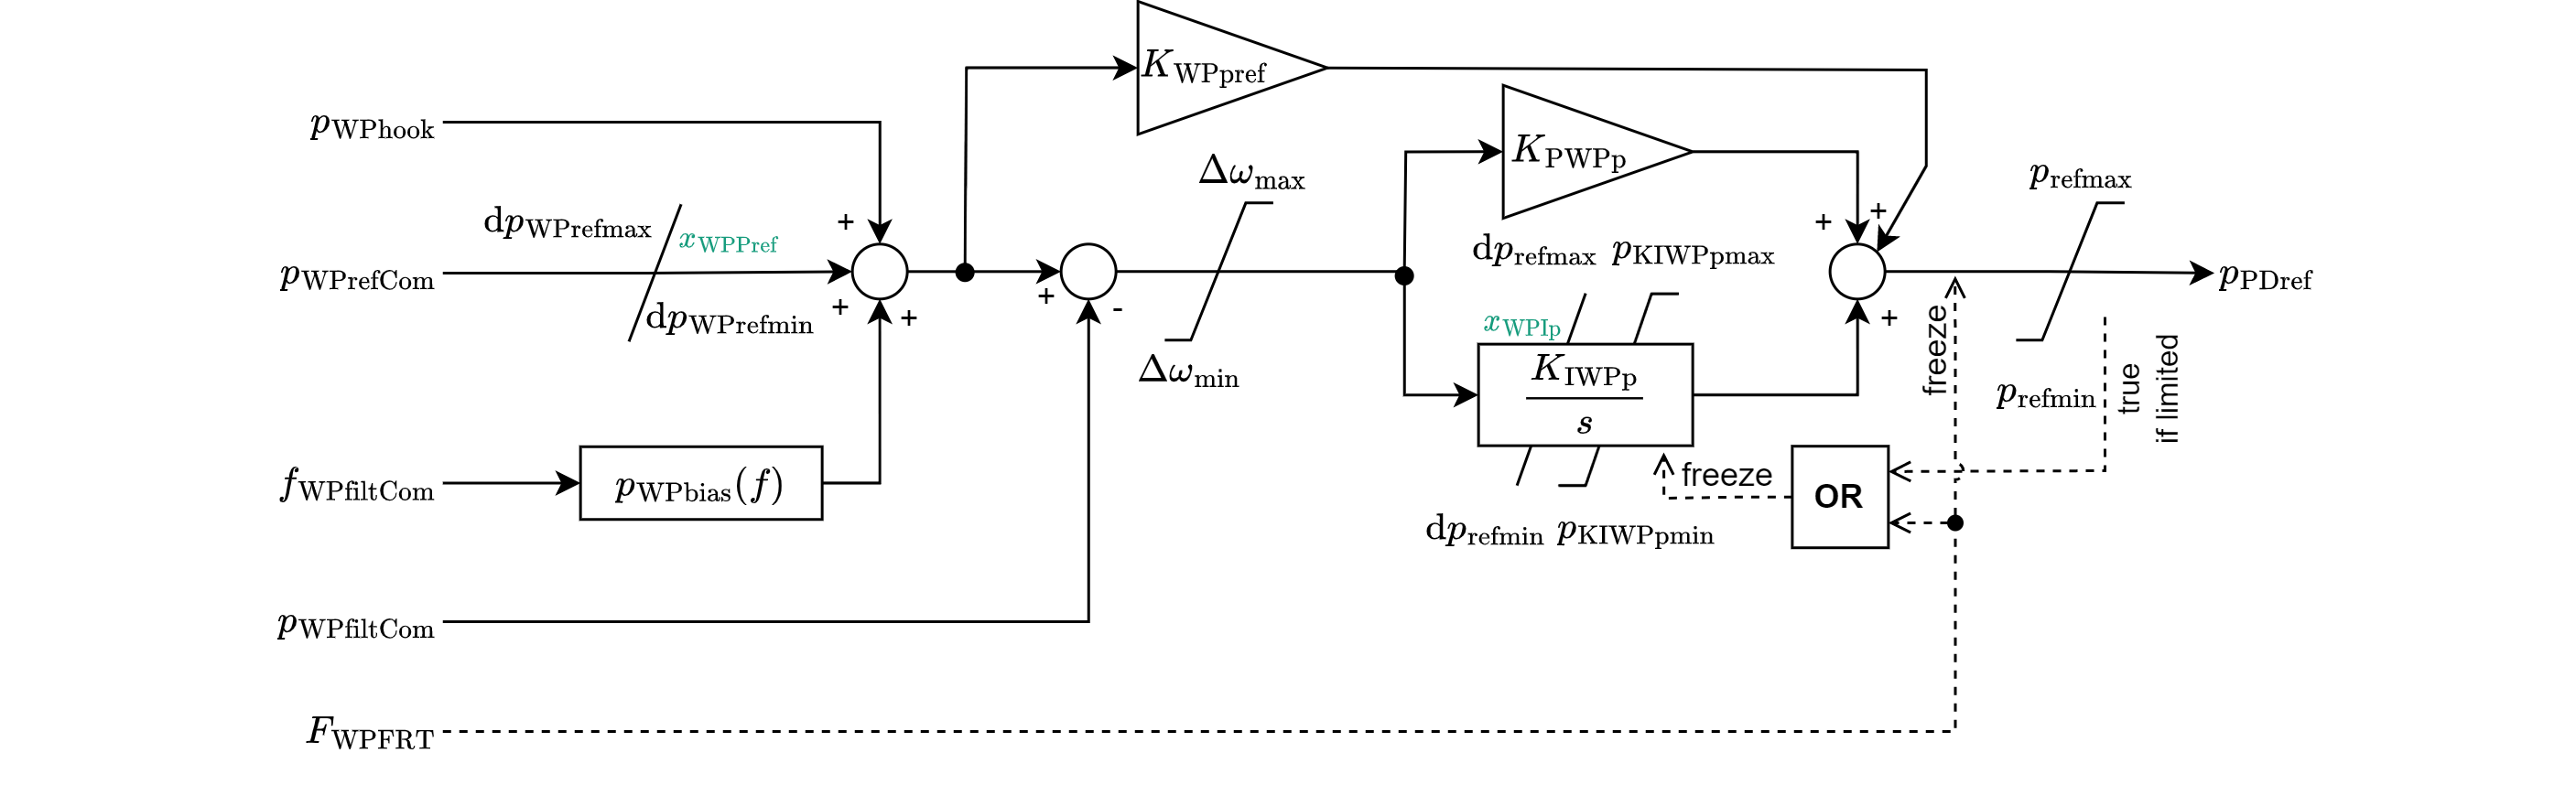
\includegraphics{drawings/WP_P.drawio.png}

}

\caption{\label{fig-wpActivePower}WPP P control module, based on
{[}1{]}}

\end{figure}%

The active power controller controls P as a function of frequency or
external reference changes {[}1{]}.

\subsubsection{Parameters}\label{parameters-8}

\begin{longtable}[]{@{}
  >{\raggedright\arraybackslash}p{(\columnwidth - 10\tabcolsep) * \real{0.1500}}
  >{\raggedright\arraybackslash}p{(\columnwidth - 10\tabcolsep) * \real{0.0800}}
  >{\raggedright\arraybackslash}p{(\columnwidth - 10\tabcolsep) * \real{0.0500}}
  >{\raggedright\arraybackslash}p{(\columnwidth - 10\tabcolsep) * \real{0.1000}}
  >{\raggedright\arraybackslash}p{(\columnwidth - 10\tabcolsep) * \real{0.4400}}
  >{\raggedright\arraybackslash}p{(\columnwidth - 10\tabcolsep) * \real{0.0700}}@{}}
\caption{Parameters of WP P control, based on {[}1{]} and
\emph{DIgSILENT PowerFactory}}\label{tbl-parametersWPP}\tabularnewline
\toprule\noalign{}
\begin{minipage}[b]{\linewidth}\raggedright
name
\end{minipage} & \begin{minipage}[b]{\linewidth}\raggedright
type
\end{minipage} & \begin{minipage}[b]{\linewidth}\raggedright
unit
\end{minipage} & \begin{minipage}[b]{\linewidth}\raggedright
base
\end{minipage} & \begin{minipage}[b]{\linewidth}\raggedright
description
\end{minipage} & \begin{minipage}[b]{\linewidth}\raggedright
typical value
\end{minipage} \\
\midrule\noalign{}
\endfirsthead
\toprule\noalign{}
\begin{minipage}[b]{\linewidth}\raggedright
name
\end{minipage} & \begin{minipage}[b]{\linewidth}\raggedright
type
\end{minipage} & \begin{minipage}[b]{\linewidth}\raggedright
unit
\end{minipage} & \begin{minipage}[b]{\linewidth}\raggedright
base
\end{minipage} & \begin{minipage}[b]{\linewidth}\raggedright
description
\end{minipage} & \begin{minipage}[b]{\linewidth}\raggedright
typical value
\end{minipage} \\
\midrule\noalign{}
\endhead
\bottomrule\noalign{}
\endlastfoot
\(\mathrm{d}p_\mathrm{refmax}\) & float & pu/s & \(S_\mathrm{base}\) &
Positive ramp rate limit of active power reference & 0.01 \\
\(\mathrm{d}p_\mathrm{refmin}\) & float & pu/s & \(S_\mathrm{base}\) &
Negative ramp rate limit of active power reference & -0.01 \\
\(\mathrm{d}p_\mathrm{WPrefmax}\) & float & pu/s & \(S_\mathrm{base}\) &
Positive ramp rate limit for power reference & 1 \\
\(\mathrm{d}p_\mathrm{WPrefmin}\) & float & pu/s & \(S_\mathrm{base}\) &
Negative ramp rate limit for power reference & -1 \\
\(K_\mathrm{IWPp}\) & float & 1/s & - & PI controller integrator gain &
1 \\
\(K_\mathrm{PWPp}\) & float & - & - & PI controller proportional gain &
0.5 \\
\(K_\mathrm{WPpref}\) & float & - & - & Gain of power reference & 0.5 \\
\(p_\mathrm{errmax}\) & float & pu & \(S_\mathrm{base}\) & PI controller
maximum control error & 1 \\
\(p_\mathrm{errmin}\) & float & pu & \(S_\mathrm{base}\) & PI controller
minimum control error & -1 \\
\(p_\mathrm{KIWPpmax}\) & float & pu & \(S_\mathrm{base}\) & PI
controller integrator upper limit & 2 \\
\(p_\mathrm{KIWPpmin}\) & float & pu & \(S_\mathrm{base}\) & PI
controller integrator lower limit & 0 \\
\(p_\mathrm{refmax}\) & float & pu & \(S_\mathrm{base}\) & Upper limit
of active power reference & 1.1 \\
\(p_\mathrm{refmin}\) & float & pu & \(S_\mathrm{base}\) & Lower limit
of active power reference & 0 \\
\(\mathbf{p_\mathrm{WPbias}}(f)\) & lookup-table & pu &
\(S_\mathrm{base}\) & Power variation as a function of frequency
(lookup-table) & {[}0,0; 1,0; 1.004,0; 1.104,-1{]} \\
\end{longtable}

\subsubsection{Variables}\label{variables-10}

\paragraph{Inputs}\label{inputs-10}

\begin{longtable}[]{@{}
  >{\raggedright\arraybackslash}p{(\columnwidth - 8\tabcolsep) * \real{0.2400}}
  >{\raggedright\arraybackslash}p{(\columnwidth - 8\tabcolsep) * \real{0.0900}}
  >{\raggedright\arraybackslash}p{(\columnwidth - 8\tabcolsep) * \real{0.0800}}
  >{\raggedright\arraybackslash}p{(\columnwidth - 8\tabcolsep) * \real{0.1900}}
  >{\raggedright\arraybackslash}p{(\columnwidth - 8\tabcolsep) * \real{0.4000}}@{}}
\caption{Inputs, based on {[}1{]}}\label{tbl-inputsWPP}\tabularnewline
\toprule\noalign{}
\begin{minipage}[b]{\linewidth}\raggedright
name
\end{minipage} & \begin{minipage}[b]{\linewidth}\raggedright
type
\end{minipage} & \begin{minipage}[b]{\linewidth}\raggedright
unit
\end{minipage} & \begin{minipage}[b]{\linewidth}\raggedright
base
\end{minipage} & \begin{minipage}[b]{\linewidth}\raggedright
description
\end{minipage} \\
\midrule\noalign{}
\endfirsthead
\toprule\noalign{}
\begin{minipage}[b]{\linewidth}\raggedright
name
\end{minipage} & \begin{minipage}[b]{\linewidth}\raggedright
type
\end{minipage} & \begin{minipage}[b]{\linewidth}\raggedright
unit
\end{minipage} & \begin{minipage}[b]{\linewidth}\raggedright
base
\end{minipage} & \begin{minipage}[b]{\linewidth}\raggedright
description
\end{minipage} \\
\midrule\noalign{}
\endhead
\bottomrule\noalign{}
\endlastfoot
\(f_\mathrm{WPfiltCom}\) & float & pu & \(f_\mathrm{n}\) & Measured
frequency \\
\(F_\mathrm{WPfiltCom}\) & boolean & - & - & WP FRT signal \\
\(p_\mathrm{WPfiltCom}\) & float & pu & \(S_\mathrm{n}\) & Measured
active power \\
\(p_\mathrm{WPhook}\) & float & pu & \(S_\mathrm{base}\) & External
active power reference offset \\
\(p_\mathrm{WPrefCom}\) & float & pu & \(S_\mathrm{base}\) & Active
power WP reference value \\
\end{longtable}

\paragraph{Outputs}\label{outputs-10}

\begin{longtable}[]{@{}
  >{\raggedright\arraybackslash}p{(\columnwidth - 8\tabcolsep) * \real{0.2400}}
  >{\raggedright\arraybackslash}p{(\columnwidth - 8\tabcolsep) * \real{0.0667}}
  >{\raggedright\arraybackslash}p{(\columnwidth - 8\tabcolsep) * \real{0.0533}}
  >{\raggedright\arraybackslash}p{(\columnwidth - 8\tabcolsep) * \real{0.2267}}
  >{\raggedright\arraybackslash}p{(\columnwidth - 8\tabcolsep) * \real{0.4133}}@{}}
\caption{Outputs, based on {[}1{]}}\label{tbl-outputsWPP}\tabularnewline
\toprule\noalign{}
\begin{minipage}[b]{\linewidth}\raggedright
name
\end{minipage} & \begin{minipage}[b]{\linewidth}\raggedright
type
\end{minipage} & \begin{minipage}[b]{\linewidth}\raggedright
unit
\end{minipage} & \begin{minipage}[b]{\linewidth}\raggedright
base
\end{minipage} & \begin{minipage}[b]{\linewidth}\raggedright
description
\end{minipage} \\
\midrule\noalign{}
\endfirsthead
\toprule\noalign{}
\begin{minipage}[b]{\linewidth}\raggedright
name
\end{minipage} & \begin{minipage}[b]{\linewidth}\raggedright
type
\end{minipage} & \begin{minipage}[b]{\linewidth}\raggedright
unit
\end{minipage} & \begin{minipage}[b]{\linewidth}\raggedright
base
\end{minipage} & \begin{minipage}[b]{\linewidth}\raggedright
description
\end{minipage} \\
\midrule\noalign{}
\endhead
\bottomrule\noalign{}
\endlastfoot
\(p_\mathrm{PDref}\) & float & pu & \(S_\mathrm{base}\) &
Power Device (PD) active power reference \\
\end{longtable}

\subsubsection{Initial equations}\label{initial-equations-6}

For the used initialization helper variables, see
Section~\ref{sec-initHelpersGlobal}.

\begin{equation}\phantomsection\label{eq-initXwppref}{
x_\mathrm{WPPref} = P_\mathrm{WTRef\,0}
}\end{equation}

\begin{equation}\phantomsection\label{eq-initXwpip}{
x_\mathrm{WPIp} = (1-K_\mathrm{WppRef})P_\mathrm{WTRef\,0}
}\end{equation}

\subsection{WP Q Control}\label{wp-q-control}

\begin{figure}

\centering{

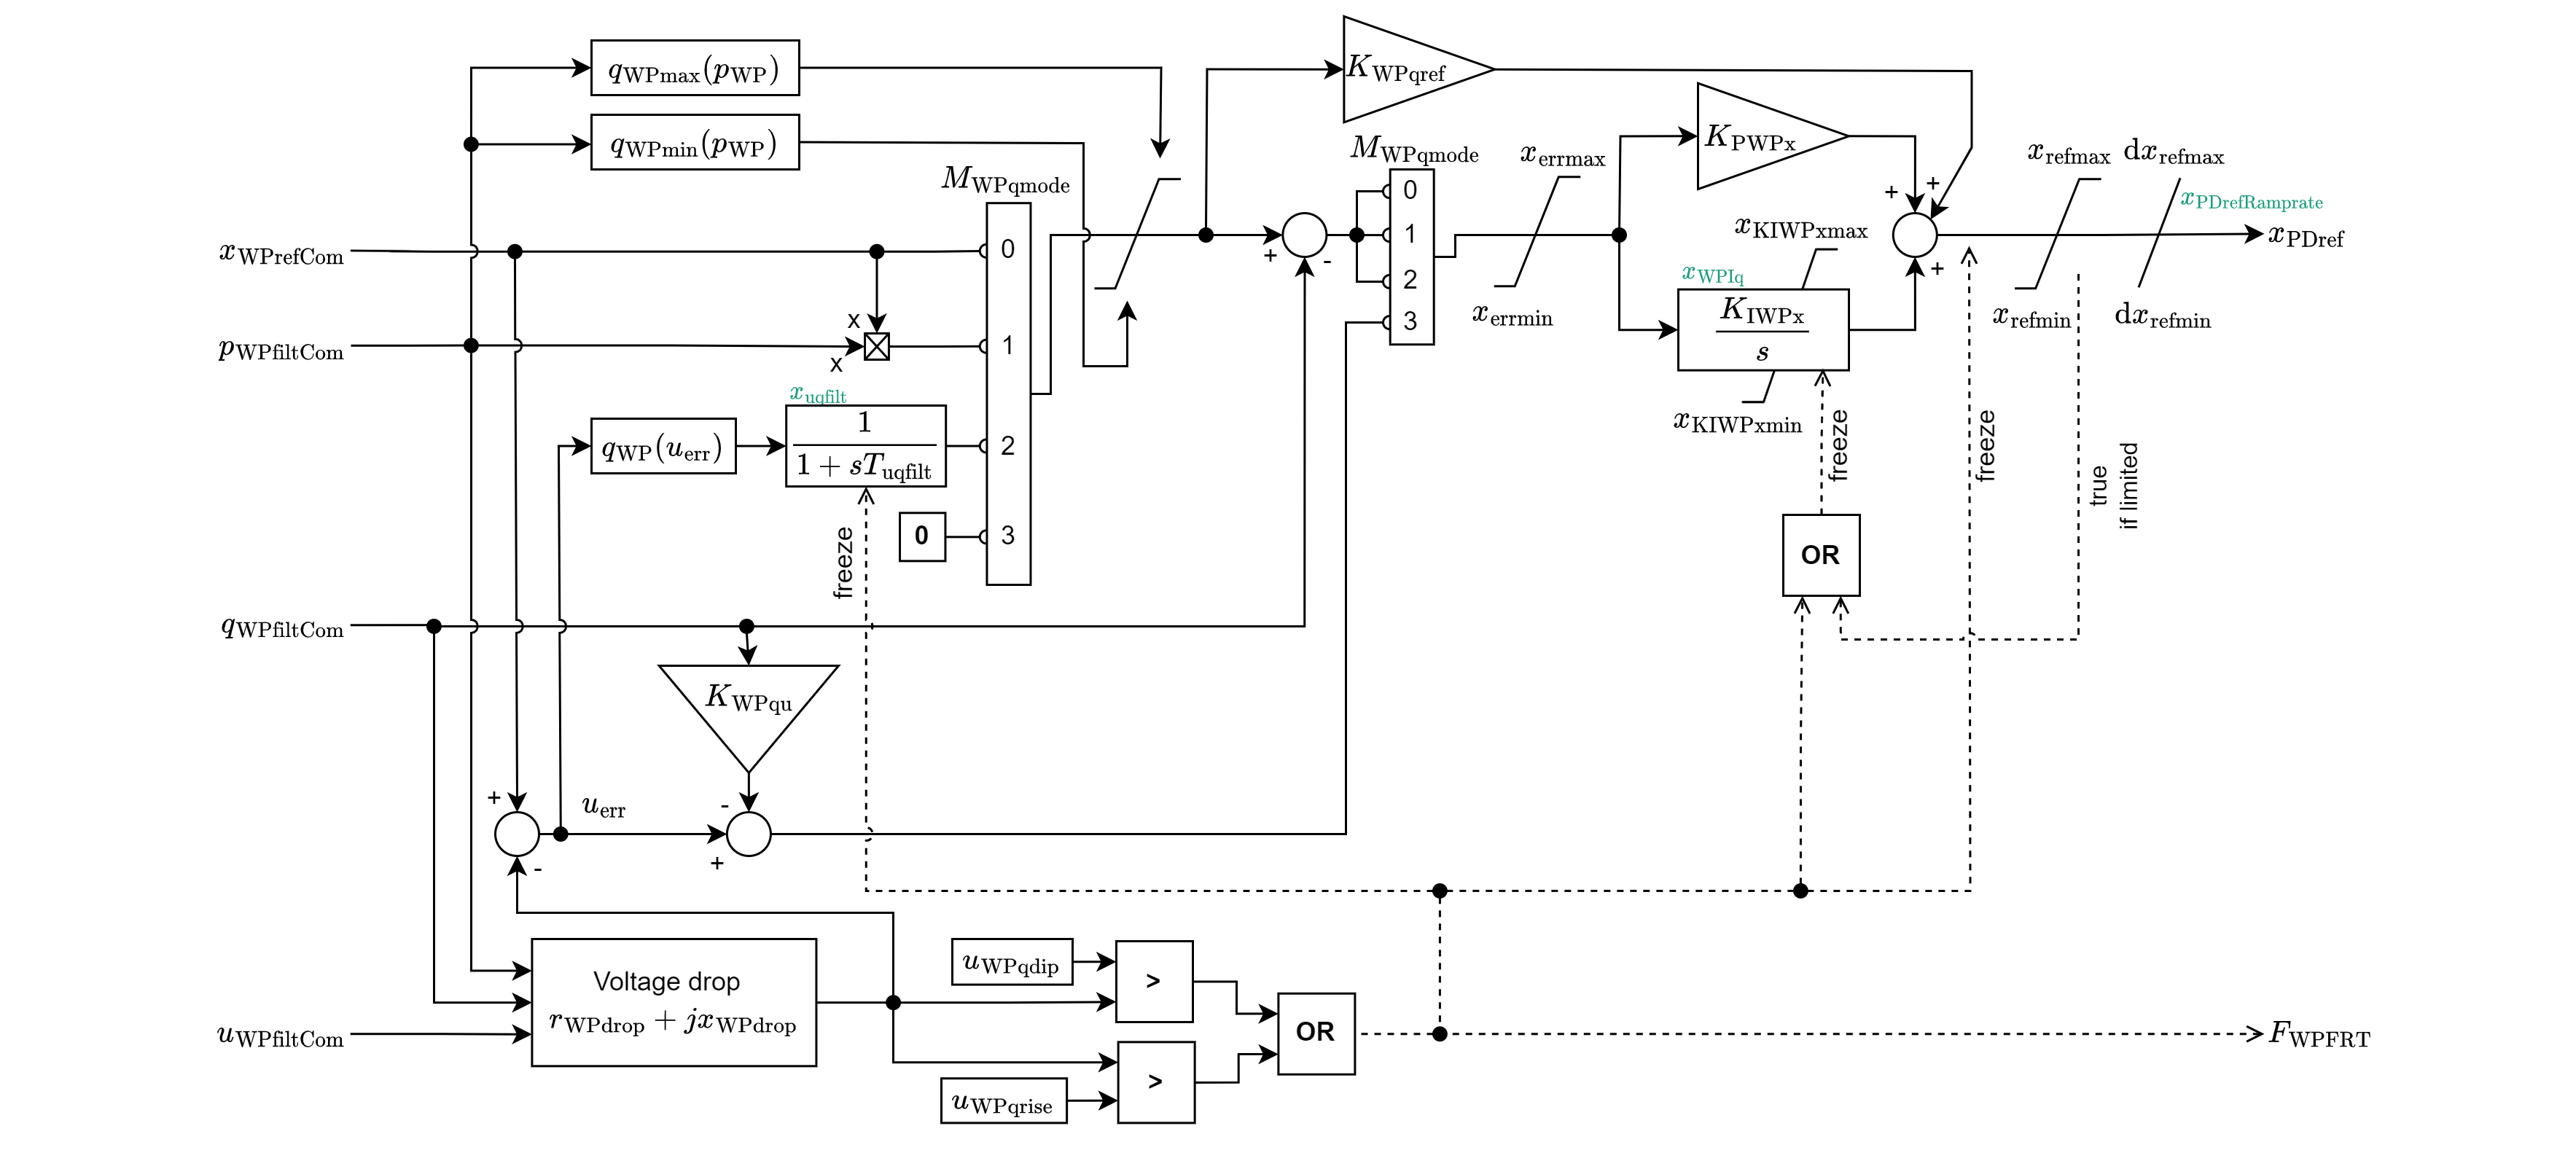
\includegraphics{drawings/WP_Q.drawio.png}

}

\caption{\label{fig-wpReactivePower}WP Q control module, based on
{[}1{]}}

\end{figure}%

The reactive power controller can control power factor, reactive power,
or voltage {[}1{]}. Reactive power capability limitations are taken into
account through the limitations in the WT model (Q limitation module).

\begin{longtable}[]{@{}
  >{\raggedright\arraybackslash}p{(\columnwidth - 10\tabcolsep) * \real{0.0600}}
  >{\raggedright\arraybackslash}p{(\columnwidth - 10\tabcolsep) * \real{0.0600}}
  >{\raggedright\arraybackslash}p{(\columnwidth - 10\tabcolsep) * \real{0.0500}}
  >{\raggedright\arraybackslash}p{(\columnwidth - 10\tabcolsep) * \real{0.2000}}
  >{\raggedright\arraybackslash}p{(\columnwidth - 10\tabcolsep) * \real{0.4400}}
  >{\raggedright\arraybackslash}p{(\columnwidth - 10\tabcolsep) * \real{0.0700}}@{}}
\caption{Parameters of WP Q control, based on {[}1{]} and
\emph{DIgSILENT PowerFactory}}\label{tbl-parametersWPQ}\tabularnewline
\toprule\noalign{}
\begin{minipage}[b]{\linewidth}\raggedright
name
\end{minipage} & \begin{minipage}[b]{\linewidth}\raggedright
type
\end{minipage} & \begin{minipage}[b]{\linewidth}\raggedright
unit
\end{minipage} & \begin{minipage}[b]{\linewidth}\raggedright
base
\end{minipage} & \begin{minipage}[b]{\linewidth}\raggedright
description
\end{minipage} & \begin{minipage}[b]{\linewidth}\raggedright
typical value
\end{minipage} \\
\midrule\noalign{}
\endfirsthead
\toprule\noalign{}
\begin{minipage}[b]{\linewidth}\raggedright
name
\end{minipage} & \begin{minipage}[b]{\linewidth}\raggedright
type
\end{minipage} & \begin{minipage}[b]{\linewidth}\raggedright
unit
\end{minipage} & \begin{minipage}[b]{\linewidth}\raggedright
base
\end{minipage} & \begin{minipage}[b]{\linewidth}\raggedright
description
\end{minipage} & \begin{minipage}[b]{\linewidth}\raggedright
typical value
\end{minipage} \\
\midrule\noalign{}
\endhead
\bottomrule\noalign{}
\endlastfoot
\(\mathrm{d}x_\mathrm{refmax}\) & float & pu/s & \(x_\mathrm{base}\) &
Positive ramp rate limit of reference value & 1 \\
\(\mathrm{d}x_\mathrm{refmin}\) & float & pu/s & \(x_\mathrm{base}\) &
Negative ramp rate limit of reference value & -1 \\
\(K_\mathrm{IWPx}\) & float & 1/s & - & PI controller integrator gain &
1 \\
\(K_\mathrm{PWPx}\) & float & - & - & PI controller proportional gain &
0.2 \\
\(K_\mathrm{WPqref}\) & float & - & - & Gain of reactive power reference
& 0.1 \\
\(K_\mathrm{WPqu}\) & float & - & - & Cross coupling gain of U
controller & 0.5 \\
\(M_\mathrm{WPqmode}\) & integer & - & - & Control mode (0 = reactive
power reference, 1 = power factor reference, 2 = Q(U) droop, 3 = voltage
reference) & 2 \\
\(\mathbf{q_\mathrm{WPmax}}(p_\mathrm{WP})\) & lookup-table & pu &
\(S_\mathrm{base}\) & Q upper limit lookup-table & {[}0,1.5;
999,1.5{]} \\
\(\mathbf{q_\mathrm{WPmin}}(p_\mathrm{WP})\) & lookup-table & pu &
\(S_\mathrm{base}\) & Q lower limit lookup-table & {[}0,-1.5;
999,-1.5{]} \\
\(\mathbf{{q_\mathrm{WP}}}(u_\mathrm{err})\) & lookup-table & pu &
\(S_\mathrm{base}\) & Q(U) static lookup-table & {[}-0.06,-0.4;
0.06,0.4{]} \\
\(r_\mathrm{WPdrop}\) & float & pu & \(Z_\mathrm{base}\) & WP voltage
drop resistance & 0 \\
\(T_\mathrm{uqfilt}\) & float & s & - & for Q(U) mode time constant &
0.01 \\
\(u_\mathrm{WPqdip}\) & float & pu & \(U_\mathrm{base}\) & UVRT
detection U threshold & 0.9 \\
\(u_\mathrm{WPqrise}\) & float & pu & \(U_\mathrm{base}\) & OVRT
detection U threshold & 1.1 \\
\(x_\mathrm{errmax}\) & float & pu & \(x_\mathrm{base}\) & Maximum
control error & 0.2 \\
\(x_\mathrm{errmin}\) & float & pu & \(x_\mathrm{base}\) & Minimum
control error & -0.2 \\
\(x_\mathrm{KIWPxmax}\) & float & pu & \(x_\mathrm{base}\) & PI
controller integrator upper limit & 1.5 \\
\(x_\mathrm{KIWPxmin}\) & float & pu & \(x_\mathrm{base}\) & PI
controller integrator lower limit & -1.5 \\
\(x_\mathrm{refmax}\) & float & pu & \(x_\mathrm{base}\) & Upper limit
of reference value & 1.3 \\
\(x_\mathrm{refmin}\) & float & pu & \(x_\mathrm{base}\) & Lower limit
of reference value & -1.3 \\
\(x_\mathrm{WPdrop}\) & float & pu & \(Z_\mathrm{base}\) & WP voltage
drop reactance & 0 \\
\end{longtable}

\subsubsection{Variables}\label{variables-11}

\paragraph{Inputs}\label{inputs-11}

\begin{longtable}[]{@{}
  >{\raggedright\arraybackslash}p{(\columnwidth - 8\tabcolsep) * \real{0.2500}}
  >{\raggedright\arraybackslash}p{(\columnwidth - 8\tabcolsep) * \real{0.0833}}
  >{\raggedright\arraybackslash}p{(\columnwidth - 8\tabcolsep) * \real{0.0833}}
  >{\raggedright\arraybackslash}p{(\columnwidth - 8\tabcolsep) * \real{0.1979}}
  >{\raggedright\arraybackslash}p{(\columnwidth - 8\tabcolsep) * \real{0.3854}}@{}}
\caption{Inputs, based on {[}1{]}}\label{tbl-inputsWPQ}\tabularnewline
\toprule\noalign{}
\begin{minipage}[b]{\linewidth}\raggedright
name
\end{minipage} & \begin{minipage}[b]{\linewidth}\raggedright
type
\end{minipage} & \begin{minipage}[b]{\linewidth}\raggedright
unit
\end{minipage} & \begin{minipage}[b]{\linewidth}\raggedright
base
\end{minipage} & \begin{minipage}[b]{\linewidth}\raggedright
description
\end{minipage} \\
\midrule\noalign{}
\endfirsthead
\toprule\noalign{}
\begin{minipage}[b]{\linewidth}\raggedright
name
\end{minipage} & \begin{minipage}[b]{\linewidth}\raggedright
type
\end{minipage} & \begin{minipage}[b]{\linewidth}\raggedright
unit
\end{minipage} & \begin{minipage}[b]{\linewidth}\raggedright
base
\end{minipage} & \begin{minipage}[b]{\linewidth}\raggedright
description
\end{minipage} \\
\midrule\noalign{}
\endhead
\bottomrule\noalign{}
\endlastfoot
\(p_\mathrm{WPfiltCom}\) & float & pu & \(S_\mathrm{base}\) & Measured
active power \\
\(q_\mathrm{WPfiltCom}\) & float & pu & \(S_\mathrm{base}\) & Measured
reactive power \\
\(u_\mathrm{WPfiltCom}\) & float & pu & \(U_\mathrm{base}\) & Measured
voltage \\
\(x_\mathrm{WPrefCom}\) & float & pu & \(x_\mathrm{base}\) & voltage or
reactive power reference \\
\end{longtable}

\paragraph{Outputs}\label{outputs-11}

\begin{longtable}[]{@{}
  >{\raggedright\arraybackslash}p{(\columnwidth - 8\tabcolsep) * \real{0.1818}}
  >{\raggedright\arraybackslash}p{(\columnwidth - 8\tabcolsep) * \real{0.0707}}
  >{\raggedright\arraybackslash}p{(\columnwidth - 8\tabcolsep) * \real{0.0404}}
  >{\raggedright\arraybackslash}p{(\columnwidth - 8\tabcolsep) * \real{0.1717}}
  >{\raggedright\arraybackslash}p{(\columnwidth - 8\tabcolsep) * \real{0.5354}}@{}}
\caption{Outputs, based on {[}1{]}}\label{tbl-outputsWPQ}\tabularnewline
\toprule\noalign{}
\begin{minipage}[b]{\linewidth}\raggedright
name
\end{minipage} & \begin{minipage}[b]{\linewidth}\raggedright
type
\end{minipage} & \begin{minipage}[b]{\linewidth}\raggedright
unit
\end{minipage} & \begin{minipage}[b]{\linewidth}\raggedright
base
\end{minipage} & \begin{minipage}[b]{\linewidth}\raggedright
description
\end{minipage} \\
\midrule\noalign{}
\endfirsthead
\toprule\noalign{}
\begin{minipage}[b]{\linewidth}\raggedright
name
\end{minipage} & \begin{minipage}[b]{\linewidth}\raggedright
type
\end{minipage} & \begin{minipage}[b]{\linewidth}\raggedright
unit
\end{minipage} & \begin{minipage}[b]{\linewidth}\raggedright
base
\end{minipage} & \begin{minipage}[b]{\linewidth}\raggedright
description
\end{minipage} \\
\midrule\noalign{}
\endhead
\bottomrule\noalign{}
\endlastfoot
\(F_\mathrm{WPFRT}\) & boolean & - & - & WP FRT signal \\
\(x_\mathrm{PDref}\) & float & pu & \(x_\mathrm{base}\) & PD voltage or
reactive power reference \\
\end{longtable}

\subsubsection{Initial equations}\label{initial-equations-7}

For the used initialization helper variables, see
Section~\ref{sec-initHelpersGlobal}.

\begin{equation}\phantomsection\label{eq-initXuqfilt}{
x_\mathrm{uqfilt} = Q_0
}\end{equation}

\begin{equation}\phantomsection\label{eq-initXwpiq}{
x_\mathrm{WPIq} = \frac{Q_\mathrm{ord\,0}}{U_0} - Q_0 \cdot K_\mathrm{WPqref}
}\end{equation}

\begin{equation}\phantomsection\label{eq-initXpdreframprate}{
x_\mathrm{PDrefRamprate} = \frac{Q_\mathrm{ord\,0}}{U_0}
}\end{equation}

\subsection{Linear communication delay
module}\label{linear-communication-delay-module}

\begin{figure}

\centering{

\includegraphics{drawings/WP_Communication.drawio.png}

}

\caption{\label{fig-wpCommunication}Linear communication delay module,
example with 3 delayed variables, based on {[}1{]}}

\end{figure}%

\subsubsection{Parameters}\label{parameters-9}

\begin{longtable}[]{@{}
  >{\raggedright\arraybackslash}p{(\columnwidth - 10\tabcolsep) * \real{0.0600}}
  >{\raggedright\arraybackslash}p{(\columnwidth - 10\tabcolsep) * \real{0.0600}}
  >{\raggedright\arraybackslash}p{(\columnwidth - 10\tabcolsep) * \real{0.0500}}
  >{\raggedright\arraybackslash}p{(\columnwidth - 10\tabcolsep) * \real{0.2000}}
  >{\raggedright\arraybackslash}p{(\columnwidth - 10\tabcolsep) * \real{0.4400}}
  >{\raggedright\arraybackslash}p{(\columnwidth - 10\tabcolsep) * \real{0.0700}}@{}}
\caption{Parameters of linear communication module, based on {[}1{]} and
\emph{DIgSILENT
PowerFactory}}\label{tbl-parametersLinearCommunictation}\tabularnewline
\toprule\noalign{}
\begin{minipage}[b]{\linewidth}\raggedright
name
\end{minipage} & \begin{minipage}[b]{\linewidth}\raggedright
type
\end{minipage} & \begin{minipage}[b]{\linewidth}\raggedright
unit
\end{minipage} & \begin{minipage}[b]{\linewidth}\raggedright
base
\end{minipage} & \begin{minipage}[b]{\linewidth}\raggedright
description
\end{minipage} & \begin{minipage}[b]{\linewidth}\raggedright
typical value
\end{minipage} \\
\midrule\noalign{}
\endfirsthead
\toprule\noalign{}
\begin{minipage}[b]{\linewidth}\raggedright
name
\end{minipage} & \begin{minipage}[b]{\linewidth}\raggedright
type
\end{minipage} & \begin{minipage}[b]{\linewidth}\raggedright
unit
\end{minipage} & \begin{minipage}[b]{\linewidth}\raggedright
base
\end{minipage} & \begin{minipage}[b]{\linewidth}\raggedright
description
\end{minipage} & \begin{minipage}[b]{\linewidth}\raggedright
typical value
\end{minipage} \\
\midrule\noalign{}
\endhead
\bottomrule\noalign{}
\endlastfoot
\(T_\mathrm{lag}\) & float & s & - & Lag time constant & 0.005 \\
\(T_\mathrm{lead}\) & float & s & - & Lead time constant & 0.005 \\
\end{longtable}

\subsubsection{Variables}\label{variables-12}

\paragraph{Inputs}\label{inputs-12}

\begin{longtable}[]{@{}
  >{\raggedright\arraybackslash}p{(\columnwidth - 8\tabcolsep) * \real{0.4923}}
  >{\raggedright\arraybackslash}p{(\columnwidth - 8\tabcolsep) * \real{0.0769}}
  >{\raggedright\arraybackslash}p{(\columnwidth - 8\tabcolsep) * \real{0.0615}}
  >{\raggedright\arraybackslash}p{(\columnwidth - 8\tabcolsep) * \real{0.0615}}
  >{\raggedright\arraybackslash}p{(\columnwidth - 8\tabcolsep) * \real{0.3077}}@{}}
\caption{Inputs, based on
{[}1{]}}\label{tbl-inputsLinearCommunication}\tabularnewline
\toprule\noalign{}
\begin{minipage}[b]{\linewidth}\raggedright
name
\end{minipage} & \begin{minipage}[b]{\linewidth}\raggedright
type
\end{minipage} & \begin{minipage}[b]{\linewidth}\raggedright
unit
\end{minipage} & \begin{minipage}[b]{\linewidth}\raggedright
base
\end{minipage} & \begin{minipage}[b]{\linewidth}\raggedright
description
\end{minipage} \\
\midrule\noalign{}
\endfirsthead
\toprule\noalign{}
\begin{minipage}[b]{\linewidth}\raggedright
name
\end{minipage} & \begin{minipage}[b]{\linewidth}\raggedright
type
\end{minipage} & \begin{minipage}[b]{\linewidth}\raggedright
unit
\end{minipage} & \begin{minipage}[b]{\linewidth}\raggedright
base
\end{minipage} & \begin{minipage}[b]{\linewidth}\raggedright
description
\end{minipage} \\
\midrule\noalign{}
\endhead
\bottomrule\noalign{}
\endlastfoot
\(y_\mathrm{1}\dots y_\mathrm{n}\) & float & any & any & number of
inputs = n \\
\end{longtable}

\paragraph{Outputs}\label{outputs-12}

\begin{longtable}[]{@{}
  >{\raggedright\arraybackslash}p{(\columnwidth - 8\tabcolsep) * \real{0.5278}}
  >{\raggedright\arraybackslash}p{(\columnwidth - 8\tabcolsep) * \real{0.0694}}
  >{\raggedright\arraybackslash}p{(\columnwidth - 8\tabcolsep) * \real{0.0556}}
  >{\raggedright\arraybackslash}p{(\columnwidth - 8\tabcolsep) * \real{0.0556}}
  >{\raggedright\arraybackslash}p{(\columnwidth - 8\tabcolsep) * \real{0.2917}}@{}}
\caption{Outputs, based on
{[}1{]}}\label{tbl-outputsLinearCommunication}\tabularnewline
\toprule\noalign{}
\begin{minipage}[b]{\linewidth}\raggedright
name
\end{minipage} & \begin{minipage}[b]{\linewidth}\raggedright
type
\end{minipage} & \begin{minipage}[b]{\linewidth}\raggedright
unit
\end{minipage} & \begin{minipage}[b]{\linewidth}\raggedright
base
\end{minipage} & \begin{minipage}[b]{\linewidth}\raggedright
description
\end{minipage} \\
\midrule\noalign{}
\endfirsthead
\toprule\noalign{}
\begin{minipage}[b]{\linewidth}\raggedright
name
\end{minipage} & \begin{minipage}[b]{\linewidth}\raggedright
type
\end{minipage} & \begin{minipage}[b]{\linewidth}\raggedright
unit
\end{minipage} & \begin{minipage}[b]{\linewidth}\raggedright
base
\end{minipage} & \begin{minipage}[b]{\linewidth}\raggedright
description
\end{minipage} \\
\midrule\noalign{}
\endhead
\bottomrule\noalign{}
\endlastfoot
\(y_\mathrm{1Com}\dots y_\mathrm{nCom}\) & float & any & any & number of
outputs = n \\
\end{longtable}

\section{Base values}\label{sec-baseValues}

The following base values are defined according to {[}1{]}:

\begin{equation}\phantomsection\label{eq-sBase}{ 
S_\mathrm{base} = 
\begin{cases}
P_\mathrm{WT\,n} &\mbox{(wind turbine nominal power) if referring to the wind turbine}\\
S_\mathrm{AUX\,n} &\mbox{(auxiliary nominal power) if referring to auxiliary components}\\
P_\mathrm{WP\,n} &\mbox{(plant nominal power) if referring to the wind power plant}
\end{cases}
}\end{equation}

\begin{equation}\phantomsection\label{eq-uBase}{ 
U_\mathrm{base} = 
\begin{cases}
U_\mathrm{WT\,n} &\mbox{(wind turbine nominal voltage) if referring to the wind turbine}\\
U_\mathrm{AUX\,n} &\mbox{(auxiliary nominal voltage) if referring to auxiliary components}\\
U_\mathrm{WP\,n} &\mbox{(plant nominal voltage) if referring to the wind power plant}
\end{cases}
}\end{equation}

\begin{equation}\phantomsection\label{eq-iBase}{ 
I_\mathrm{base} = \dfrac{S_\mathrm{base}}{\sqrt{3}U_\mathrm{base}}
}\end{equation}

\begin{equation}\phantomsection\label{eq-zBase}{ 
Z_\mathrm{base} = \dfrac{U_\mathrm{base}^2}{S_\mathrm{base}}
}\end{equation}

\begin{equation}\phantomsection\label{eq-omegaBase}{ 
\Omega_\mathrm{base} = 
\begin{cases}
\omega_\mathrm{n} &\mbox{if referring to generator}\\
\dfrac{\omega_\mathrm{n}}{n_\mathrm{gearbox}} & \mbox{if referring to wind turbine rotor}
\end{cases}
}\end{equation}

\begin{equation}\phantomsection\label{eq-tBase}{ 
T_\mathrm{base} = \dfrac{P_\mathrm{WT\,n}}{\Omega_\mathrm{base}} \mbox{ (use turbine nominal power)}
}\end{equation}

\begin{equation}\phantomsection\label{eq-xBase}{ 
x_\mathrm{base} = 
\begin{cases}
S_\mathrm{base} &\mbox{if in reactive power control mode}\\
U_\mathrm{base} &\mbox{if in voltage control mode}
\end{cases}
}\end{equation}

\section{Operating point and initialization
helpers}\label{sec-initHelpersGlobal}

\begin{longtable}[]{@{}ll@{}}
\caption{Initial operating point parameters}\tabularnewline
\toprule\noalign{}
Operating point parameter & Description \\
\midrule\noalign{}
\endfirsthead
\toprule\noalign{}
Operating point parameter & Description \\
\midrule\noalign{}
\endhead
\bottomrule\noalign{}
\endlastfoot
\(P_\mathrm{0}\) & Active power at point of connection \\
\(U_\mathrm{0}\) & Voltage magnitude at point of connection \\
\(\varphi_\mathrm{0}\) & Voltage angle at point of connection \\
\(Q_\mathrm{0}\) & Reactive power at point of connection \\
\(\omega_0\) & Grid frequency (typically 1 pu) \\
\(P_\mathrm{WTRef\,0}\) & Active power setpoint \\
\(\underline{Z}\) & Connection impedance \\
\(\underline{Y}\) & Connection admittance \\
\end{longtable}

\begin{equation}\phantomsection\label{eq-u0}{
\underline{u}_0 =  U_0 \exp (\mathrm{j}\varphi_\mathrm{0})
}\end{equation}

\begin{equation}\phantomsection\label{eq-i0}{
\underline{i}_0 =  ((P_0 + \mathrm{j}Q_0)/\underline{u}_0)^*
}\end{equation}

\begin{equation}\phantomsection\label{eq-ugs0}{
U_\mathrm{gs\,re\,0} + \mathrm{j}U_\mathrm{gs\,im\,0} = \underline{u}_\mathrm{gs\,0} = \underline{u}_0 - \underline{Z} \cdot \underline{i}_0
}\end{equation}

\begin{equation}\phantomsection\label{eq-igs0}{
I_\mathrm{gs\,re\,0} + \mathrm{j}I_\mathrm{gs\,im\,0} = \underline{i}_\mathrm{gs\,0} = \underline{i}_0 - \underline{Y} \cdot \underline{u}_\mathrm{gs\,0}
}\end{equation}

\begin{equation}\phantomsection\label{eq-initPOrd}{
P_\mathrm{ord\,0} = 
\begin{cases}
    P_\mathrm{0} & \text{for Type 3A}\\
    U_\mathrm{0} \cdot ((I_\mathrm{gs\,re\,0} + \frac{U_\mathrm{gs\,im\,0}}{X_\mathrm{eqv}})\cos(\varphi_\mathrm{u\,0}) + (I_\mathrm{gs\,im\,0} - \frac{U_\mathrm{gs\,re\,0}}{X_\mathrm{eqv}})\sin(\varphi_\mathrm{u\,0})) & \text{for Type 3B}
\end{cases}
}\end{equation}

\begin{equation}\phantomsection\label{eq-initQOrd}{
Q_\mathrm{ord\,0} = 
\begin{cases}
    Q_\mathrm{0} & \text{for Type 3A}\\
    -U_\mathrm{0} \cdot ((I_\mathrm{gs\,re\,0} + \frac{U_\mathrm{gs\,im\,0}}{X_\mathrm{eqv}})\sin(\varphi_\mathrm{u\,0}) - (I_\mathrm{gs\,im\,0} - \frac{U_\mathrm{gs\,re\,0}}{X_\mathrm{eqv}})\cos(\varphi_\mathrm{u\,0}) &~\\ 
    + \frac{\sqrt{U_\mathrm{gs\,re\,0}^2+U_\mathrm{gs\,im\,0}^2}}{X_\mathrm{eqv}}) & \text{for Type 3B}
\end{cases}
}\end{equation}

\begin{equation}\phantomsection\label{eq-initPAg}{
P_\mathrm{ag\,0} = \Re \left( (U_\mathrm{gs\,re\,0}+ \mathrm{j}U_\mathrm{gs\,im\,0}) \cdot (I_\mathrm{gs\,re\,0}- \mathrm{j}I_\mathrm{gs\,im\,0}) \right)
}\end{equation}

\section{Open questions}\label{open-questions}

\begin{itemize}
\tightlist
\item
  Why is u/xeqv added to iq command in Type 3B generator system?
\item
  It remained unclear to the autors what the torque PI input
  \(u_\mathrm{TChook}\) represents in the P Controller.
\end{itemize}

\section{Information about Dynawo implementation
(modelica)}\label{information-about-dynawo-implementation-modelica}

\begin{longtable}[]{@{}
  >{\raggedright\arraybackslash}p{(\columnwidth - 2\tabcolsep) * \real{0.3496}}
  >{\raggedright\arraybackslash}p{(\columnwidth - 2\tabcolsep) * \real{0.6504}}@{}}
\caption{Necessary sub models and their availability in
Dynawo}\label{tbl-availability_in_dynawo}\tabularnewline
\toprule\noalign{}
\begin{minipage}[b]{\linewidth}\raggedright
Sub model
\end{minipage} & \begin{minipage}[b]{\linewidth}\raggedright
Name in Dynawo
\end{minipage} \\
\midrule\noalign{}
\endfirsthead
\toprule\noalign{}
\begin{minipage}[b]{\linewidth}\raggedright
Sub model
\end{minipage} & \begin{minipage}[b]{\linewidth}\raggedright
Name in Dynawo
\end{minipage} \\
\midrule\noalign{}
\endhead
\bottomrule\noalign{}
\endlastfoot
WT Pitch angle control module & Dynawo .Electrical .Controls .IEC
.IEC61400 .BaseControls .WT .PitchAngleControl \\
WT Two-dimensional aerodynamic module & Dynawo .Electrical .Controls
.IEC .IEC61400 .BaseControls .WT .Aerodynamic2d \\
WT Two mass mechanical module & Dynawo .Electrical .Controls .IEC
.BaseControls .WT .Mechanical \\
WT Grid measurement module & Dynawo .Electrical .Controls .IEC
.BaseControls .Auxiliaries .Measurements \\
WT Generator control sub-structure (Type 3) & Dynawo .Electrical
.Controls .IEC .IEC61400 .WT .Control3AB2020 \\
WT P control module (Type 3) & Dynawo .Electrical .Controls .IEC
.IEC61400 .BaseControls .WT .PControl3AB2020 \\
WT Torque PI block (Type 3) & Dynawo .Electrical .Controls .IEC
.IEC61400 .BaseControls .WT .TorquePi \\
WT Q control module & Dynawo .Electrical .Controls .IEC .BaseControls
.WT .QControl2020 \\
WT Current limitation module & Dynawo .Electrical .Controls .IEC
.BaseControls .WT .CurrentLimiter2020 \\
WT Q limitation module & Dynawo .Electrical .Controls .IEC .BaseControls
.WT .QLimiter2020 \\
WT Generator system Type 3A & Dynawo .Electrical .Sources .IEC
.BaseConverters .GenSystem3a \\
WT Generator system Type 3B & Dynawo .Electrical .Sources .IEC
.BaseConverters .GenSystem3b \\
WT Grid protection system module & Dynawo .Electrical .Controls .IEC
.BaseControls .Auxiliaries .GridProtection2020 \\
WT Electrical system & Dynawo .Electrical .Sources .IEC .BaseConverters
.ElecSystem \\
WP control and communication module & Dynawo .Electrical .Controls .IEC
.WPP .WPPControl \\
WP P control & Dynawo .Electrical .Controls .IEC .BaseControls .WPP
.QControl \\
WP Q control & Dynawo .Electrical .Controls .IEC .BaseControls .WPP
.PControl \\
Linear communication module & Dynawo .Electrical .Controls .IEC
.BaseControls .WPP .LinearCommunication \\
Communication delay module & - (in development by RTE) \\
\end{longtable}

\subsection{Torque PI block (Type 3)}\label{torque-pi-block-type-3}

\begin{itemize}
\tightlist
\item
  the rate limiter that limits \(\tau_\mathrm{reset}\) in
  Figure~\ref{fig-torquePi} is implemented using a fast first-order lag.
  Its time constant needs to be very fast. Otherwise, the set function
  does not behave as desired.
\end{itemize}

\subsection{Pitch angle control block}\label{pitch-angle-control-block}

While the IEC standard defines integrator gain parameters for the speed
and power integrators, the dynamics of the anti-windup integrators in
Dynawo are defined by the integration time constant. If the integration
time constant is set to be \(1/K_\mathrm{I}\), the gain value cannot be
zero. Therefore, the typical value of \(K_\mathrm{Ic}\) needs to be
changed to a very small number (e.g.~1e-9) instead of zero.

\section{Table of references}\label{table-of-references}

\phantomsection\label{refs}
\begin{CSLReferences}{0}{0}
\bibitem[\citeproctext]{ref-iec2020}
\CSLLeftMargin{{[}1{]} }%
\CSLRightInline{{``{IEC} 61400-27-1 {Wind Energy Generation Systems} --
{Part27} -- {Electrical} simulation models -- {Generic} models.''} Jul.
2020.}

\bibitem[\citeproctext]{ref-honrubia-escribano2018}
\CSLLeftMargin{{[}2{]} }%
\CSLRightInline{A. Honrubia-Escribano, E. Gómez-Lázaro, J. Fortmann, P.
Sørensen, and S. Martin-Martinez, {``Generic dynamic wind turbine models
for power system stability analysis: {A} comprehensive review,''}
\emph{Renewable and Sustainable Energy Reviews}, vol. 81, pp.
1939--1952, Jan. 2018, doi:
\href{https://doi.org/10.1016/j.rser.2017.06.005}{10.1016/j.rser.2017.06.005}.}

\bibitem[\citeproctext]{ref-fortmann2014}
\CSLLeftMargin{{[}3{]} }%
\CSLRightInline{J. Fortmann, \emph{Modeling of wind turbines with doubly
fed generator system}. Wiesbaden: Springer Vieweg, 2014. doi:
\href{https://doi.org/10.1007/978-3-658-06882-0}{10.1007/978-3-658-06882-0}.}

\bibitem[\citeproctext]{ref-fortmann2014a}
\CSLLeftMargin{{[}4{]} }%
\CSLRightInline{J. Fortmann, S. Engelhardt, J. Kretschmann, C. Feltes,
and I. Erlich, {``New {Generic Model} of {DFG-Based Wind Turbines} for
{RMS-Type Simulation},''} \emph{IEEE Transactions on Energy Conversion},
vol. 29, no. 1, pp. 110--118, Mar. 2014, doi:
\href{https://doi.org/10.1109/TEC.2013.2287251}{10.1109/TEC.2013.2287251}.}

\bibitem[\citeproctext]{ref-lorenzo-bonache2017}
\CSLLeftMargin{{[}5{]} }%
\CSLRightInline{A. Lorenzo-Bonache, A. Honrubia-Escribano, F.
Jiménez-Buendía, Á. Molina-García, and E. Gómez-Lázaro, {``Generic
{Type} 3 {Wind Turbine Model Based} on {IEC} 61400-27-1: {Parameter
Analysis} and {Transient Response} under {Voltage Dips},''}
\emph{Energies}, vol. 10, no. 9, 9, p. 1441, Sep. 2017, doi:
\href{https://doi.org/10.3390/en10091441}{10.3390/en10091441}.}

\bibitem[\citeproctext]{ref-lorenzo-bonache2019}
\CSLLeftMargin{{[}6{]} }%
\CSLRightInline{A. Lorenzo-Bonache, A. Honrubia-Escribano, J. Fortmann,
and E. Gómez-Lázaro, {``Generic {Type} 3 {WT} models: Comparison between
{IEC} and {WECC} approaches,''} \emph{IET Renewable Power Generation},
vol. 13, no. 7, pp. 1168--1178, 2019, doi:
\href{https://doi.org/10.1049/iet-rpg.2018.6098}{10.1049/iet-rpg.2018.6098}.}

\bibitem[\citeproctext]{ref-franke2024}
\CSLLeftMargin{{[}7{]} }%
\CSLRightInline{M. Franke, A. Guironnet, and C. Cardozo, {``Comparing
{IEC} and {WECC Generic Dynamic Models} for {Type} 4 {Wind Turbines},''}
2024.}

\bibitem[\citeproctext]{ref-tsourakis2009}
\CSLLeftMargin{{[}8{]} }%
\CSLRightInline{G. Tsourakis, B. M. Nomikos, and C. D. Vournas,
{``Contribution of {Doubly Fed Wind Generators} to {Oscillation
Damping},''} \emph{IEEE Trans. Energy Convers.}, vol. 24, no. 3, pp.
783--791, Sep. 2009, doi:
\href{https://doi.org/10.1109/TEC.2009.2025330}{10.1109/TEC.2009.2025330}.}

\end{CSLReferences}




\end{document}
